\documentclass[12pt,a4paper]{report}
% \usepackage[english, vietnam]{babel}
\usepackage[T5,T1]{fontenc}
\usepackage{mathptmx}[ptm]
%\usepackage[utf8]{inputenc}
\usepackage[utf8]{vietnam}
%\usepackage[francais]{babel}
\usepackage{a4wide,amssymb,epsfig,latexsym,array,hhline,fancyhdr}
\usepackage[vietnamese]{babel}
\usepackage{csquotes}
\usepackage[style=apa, citestyle=numeric, backend=biber, sorting=none]{biblatex}
\bibliography{refs}
% \usepackage{apacite}
\usepackage[toc,page]{appendix}
\usepackage{pifont,amssymb}
\newcommand{\emptysquare}{$\square$}
\newcommand{\checkedsquare}{\makebox[0pt][l]{\raisebox{1pt}[0pt][0pt]{\large\hspace{1pt}\cmark}}$\square$}
\newcommand{\cmark}{\ding{51}}

\DeclareFieldFormat{labelnumberwidth}{\mkbibbrackets{#1}}

\defbibenvironment{bibliography}
  {\list
     {\printtext[labelnumberwidth]{%
      \printfield{labelprefix}%
      \printfield{labelnumber}}}
     {\setlength{\labelwidth}{\labelnumberwidth}%
      \setlength{\leftmargin}{\labelwidth}%
      \setlength{\labelsep}{\biblabelsep}%
      \addtolength{\leftmargin}{\labelsep}%
      \setlength{\itemsep}{\bibitemsep}%
      \setlength{\parsep}{\bibparsep}}%
      \renewcommand*{\makelabel}[1]{\hss##1}}
  {\endlist}
  {\item}


\addbibresource{newrefs.bib}
% \newcommand*{\captionsource}[2]{%
% \centering
%   \caption[{#1}]{%
%     #1%
%     \\\hspace{\linewidth}%
%     \textbf{Source:} #2%
%   }%
% }

\usepackage{vcell}
\usepackage{tabularray}
%\usepackage{soul}

\usepackage[makeroom]{cancel}
\usepackage{amsmath}
\usepackage{amsthm}
\usepackage{multicol,longtable,amscd}
\usepackage{diagbox}%Make diagonal lines in tables
\usepackage{booktabs}
\usepackage{alltt}
\usepackage[framemethod=tikz]{mdframed}% For highlighting paragraph backgrounds
\usepackage{caption,subcaption}
\usepackage{float}
\usepackage{lastpage}
\usepackage[lined,boxed,commentsnumbered]{algorithm2e}
\usepackage{enumerate}
\usepackage{color}
\usepackage{graphicx}							% Standard graphics package
\usepackage{array}
\usepackage{tabularx, caption}
\usepackage{multirow}
\usepackage{multicol}
\usepackage{enumitem}
\usepackage{rotating}
\usepackage{graphics}
\usepackage{geometry}
\usepackage{setspace}
\usepackage{epsfig}
\usepackage{tikz}
\usepackage{titlesec}
\usepackage{url}
\usepackage{ragged2e}
\usepackage{makecell}
% \usepackage[style=apa]{biblatex}
% \usepackage{natbib}
% \bibliographystyle{ieeetr}

\usetikzlibrary{arrows,snakes,backgrounds,calc}
\usepackage{hyperref}
\hypersetup{urlcolor=blue,linkcolor=black,citecolor=black,colorlinks=true}
\usepackage{listings}

\lstdefinelanguage{JSON}{
    morestring=[b]",
    morestring=[b]',
    morecomment=[s]{/*}{*/},
    morecomment=[l]//,
    literate=
        *{0}{{{\color{red}0}}}{1}
         {1}{{{\color{red}1}}}{1}
         {2}{{{\color{red}2}}}{1}
         {3}{{{\color{red}3}}}{1}
         {4}{{{\color{red}4}}}{1}
         {5}{{{\color{red}5}}}{1}
         {6}{{{\color{red}6}}}{1}
         {7}{{{\color{red}7}}}{1}
         {8}{{{\color{red}8}}}{1}
         {9}{{{\color{red}9}}}{1}
         {:}{{{\color{blue}:}}}{1}
         {,}{{{\color{blue},}}}{1}
         {\{}{{{\color{blue}\{}}}{1}
         {\}}{{{\color{blue}\}}}}{1}
         {[}{{{\color{blue}[}}}{1}
         {]}{{{\color{blue}]}}}{1},
    sensitive=false,
    keywords={true,false,null},
    keywordstyle=\color{purple}\bfseries,
    stringstyle=\color{orange},
    commentstyle=\color{gray}\itshape
}

% Cài đặt cho listings (mã nguồn)
\lstset{
    basicstyle=\ttfamily\small,
    breaklines=true,
    frame=single,
    keywordstyle=\color{blue},
    commentstyle=\color{gray},
    stringstyle=\color{red}
}
%\usepackage{pstcol} 								% PSTricks with the standard color package

\usepackage[normalem]{ulem}

\newtheorem{theorem}{{\bf Định lý}}
\newtheorem{property}{{\bf Tính chất}}
\newtheorem{proposition}{{\bf Mệnh đề}}
\newtheorem{corollary}[proposition]{{\bf Hệ quả}}
\newtheorem{lemma}[proposition]{{\bf Bổ đề}}
\theoremstyle{definition}
\newtheorem{exer}{Bài toán}

\def\thesislayout{	% A4: 210 × 297
	\geometry{
		a4paper,
		total={160mm,240mm},  % fix over page
		left=30mm,
		top=30mm,
	}
}
\def\thesisheadlayout{	% A4: 210 × 297
	\geometry{
		a4paper,
		total={160mm,240mm},  % fix over page
		left=30mm,
		top=10mm,
	}
}
\thesislayout
\lstset{
    language=R,
    basicstyle=\footnotesize\sffamily,
    commentstyle=\ttfamily\color{black},
    numbers=left,
    numberstyle=\ttfamily\color{black}\footnotesize,
    stepnumber=1,
    numbersep=5pt,
    backgroundcolor=\color{white},
    showspaces=false,
    showstringspaces=false,
    showtabs=false,
    frame=single,
    tabsize=2,
    captionpos=b,
    breaklines=true,
    breakatwhitespace=false,
    title=\lstname,
    escapeinside={},
    keywordstyle={},
    morekeywords={}
}
%\usepackage{fancyhdr}
\setlength{\headheight}{40pt}
\pagestyle{fancy}
\fancyhead{} % clear all header fields
\fancyhead[L]{
 \begin{tabular}{rl}
    \begin{picture}(25,15)(0,0)
    \put(0,-8){
\includegraphics[width=12mm, height=12mm]{images/hcmut.png}}
    %\put(0,-8){\epsfig{width=10mm,figure=hcmut.eps}}
   \end{picture}&
	%
\includegraphics[width=12mm, height=12mm]{hcmut.png} & %
	\begin{tabular}{l}
		\textbf{  Ho Chi Minh City University of Technology }\\
		\textbf{  Faculty of Computer Science and Engineering }
	\end{tabular} 	
 \end{tabular}
}
\fancyhead[R]{
	\begin{tabular}{l}
		\tiny \bf \\
		\tiny \bf 
	\end{tabular}  }
\fancyfoot{} % clear all footer fields
\fancyfoot[L]{\scriptsize  Specialized project report}
\fancyfoot[R]{\scriptsize  Page {\thepage}/\pageref{LastPage}}
\renewcommand{\headrulewidth}{0.3pt}
\renewcommand{\footrulewidth}{0.3pt}


%%%
\setcounter{secnumdepth}{4}
\setcounter{tocdepth}{3}
\makeatletter
\newcounter {subsubsubsection}[subsubsection]
\renewcommand\thesubsubsubsection{\thesubsubsection .\@alph\c@subsubsubsection}
\newcommand\subsubsubsection{\@startsection{subsubsubsection}{4}{\z@}%
                                     {-3.25ex\@plus -1ex \@minus -.2ex}%
                                     {1.5ex \@plus .2ex}%
                                     {\normalfont\normalsize\bfseries}}
\newcommand*\l@subsubsubsection{\@dottedtocline{3}{7.0em}{4.1em}}
\newcommand*{\subsubsubsectionmark}[1]{}
\makeatother

\everymath{\color{black}}%make in-line maths symbols blue to read/check easily

\sloppy
\captionsetup[figure]{labelfont={small,bf},textfont={small,it},belowskip=-1pt,aboveskip=5pt}
%space remove between caption, figure, and text
\captionsetup[table]{labelfont={small,bf},textfont={small,it},belowskip=-1pt,aboveskip=7pt}
\setlength{\floatsep}{5pt plus 2pt minus 2pt}
\setlength{\textfloatsep}{5pt plus 2pt minus 2pt}
\setlength{\intextsep}{10pt plus 2pt minus 2pt}
\DeclareTextFontCommand{\textvietnamese}{\fontencoding{T5}\selectfont}

\thesislayout

%% Spacings
\onehalfspacing     % spacing between lines
\setlength{\parskip}{7.5pt} % between paragraphs
\setlength{\parindent}{7pt} % new para indentation
\titlespacing*{\section}{0pt}{0pt}{0pt}
\titlespacing*{\subsection}{0pt}{0pt}{0pt}
\titlespacing*{\subsubsection}{0pt}{0pt}{0pt}

%%%%%%%%%%%%%%%%%%%%%%%%%%%%%%%%%%%%%%%%%%%%%%%%%%%%%%%%%%%%%%%%%%%%%%%%%
\begin{document}
\begin{titlepage}
	\begin{tikzpicture}[remember picture, overlay]
		\draw[line width = 4pt] ($(current page.north west) + (0.4in,-0.5in)$) rectangle ($(current page.south east) + (-0.4in,0.5in)$);
		\draw[line width=1.5pt]
		($ (current page.north west) + (0.45in,-0.55in) $)
		rectangle
		($ (current page.south east) + (-0.45in,0.55in) $);
	\end{tikzpicture}

	\begin{singlespace}
		\vspace{-2cm}
		\begin{center}
			\fontsize{15}{12} \textbf{ĐẠI HỌC QUỐC GIA THÀNH PHỐ HỒ CHÍ MINH} \\
			\vspace{0.2cm}
			\fontsize{15}{12} \textbf{TRƯỜNG ĐẠI HỌC BÁCH KHOA} \\
			\vspace{0.2cm}
			\fontsize{15}{12} \textbf{KHOA KHOA HỌC VÀ KỸ THUẬT MÁY TÍNH}
		\end{center}
	\end{singlespace}

	\vspace{0.2cm}

	\begin{figure}[h!]
		\begin{center}
			
\includegraphics[width=5cm]{images/hcmut.png}
		\end{center}
	\end{figure}

	\vspace{0.3cm}

	\begin{center}
		\fontsize{15}{12} \textbf{Đồ án tốt nghiệp}  \\
		\fontsize{15}{12} \textbf{BÁO CÁO}  \\
	\end{center}

	\vspace{0.5cm}

	\begin{center}
		\setstretch{1.9}\fontsize{23}{12} \textbf{XÂY DỰNG HỆ THỐNG GIÁO DỤC THÔNG MINH DỰA TRÊN MÔ HÌNH NGÔN NGỮ LỚN} \\
		\vspace{0.5em}
		\fontsize{15}{12}\selectfont Ngành: Khoa học máy tính \\
	\end{center}

	\vspace{0.5cm}

	\begin{center}
		\fontsize{15}{12}\selectfont{
			\renewcommand{\arraystretch}{1.3}
			\begin{tabular}{rl}
				\textbf{THESIS COMMITTEE:} &                                    \\
				\textbf{GVHD 1:}           & Assoc. Prof. Võ Thị Ngọc Châu, PhD \\
				\textbf{GVHD 2:}           & Assoc. Prof. Nguyễn Hứa Phùng, PhD \\
				\multicolumn{2}{c}{\textbf{---o0o---}}                          \\

				\textbf{Sinh viên 1}:      & Phan Phạm Thi (2114857)            \\
				\textbf{Sinh viên 2:}      & Nguyễn Trường Tuấn Anh (2112796)   \\   \textbf{Sinh viên 3:} & Đỗ Phương Nam (2114111)
			\end{tabular}
		}
	\end{center}

	\vspace{2.2cm}

	\begin{center}
		\fontsize{15}{12}\selectfont Ho Chi Minh City, June 2024
	\end{center}
\end{titlepage}



% \vspace{2\baselineskip}

% \noindent\rule{4in}{0.7pt} \hfill \rule{1.5in}{0.7pt}

% \noindent Darth Sion\\
% Professor, Department of Chemistry and Biochemistry\\
% University of Sichuan Gourmet Kitchen\\
% Thesis Committee

% \vspace{2\baselineskip}

% (etc.)
\newpage
\begin{center}
	\textbf{\Large PROTESTATION} \par
\end{center}
Báo cáo này được thực hiện với mục tiêu triển khai và phát triển hoàn chỉnh các tính năng của hệ thống học tập trực tuyến thông minh, nhằm đáp ứng nhu cầu học tập cá nhân hóa và tối ưu hóa quá trình học của sinh viên ngành Khoa học máy tính. Trong suốt quá trình thực hiện, nhóm đã gặp phải không ít thử thách, từ việc tối ưu hóa các thuật toán học máy cho đến việc triển khai các tính năng AI trong hệ thống. Tuy nhiên, với sự nỗ lực không ngừng và sự hỗ trợ từ các nguồn tài liệu cũng như người hướng dẫn, nhóm đã hoàn thành mục tiêu phát triển hệ thống như đã đề ra.

Mặc dù đã đạt được nhiều thành công ở giai đoạn 1, nhóm cũng nhận thức rằng một số tính năng trong hệ thống vẫn cần được cải tiến thêm, đặc biệt trong việc tối ưu hóa tốc độ xử lý và tính chính xác của các đề xuất học tập. Tuy nhiên, những khó khăn này sẽ là cơ sở để nhóm tiếp tục hoàn thiện hệ thống trong giai đoạn 2 này.

Chúng tôi cam kết rằng báo cáo này là công trình nghiên cứu độc lập của nhóm. Tất cả các kết quả nghiên cứu, dữ liệu thu thập và phân tích đều được thực hiện một cách trung thực và không sao chép từ bất kỳ công trình nghiên cứu nào trước đó. Mọi nguồn tài liệu tham khảo đều được trích dẫn đầy đủ và rõ ràng trong báo cáo này.
\par\hfill\textbf{Authors}\hspace{1cm}

\par\hfill\textit{Phan Phạm Thi}\hspace{0.3cm}
\par\hfill\textit{Nguyễn Trường Tuấn Anh}\hspace{0.2cm}\par\hfill\textit{Đỗ Phương Nam}
\newpage

\begin{center}
	\textbf{\Large ACKNOWLEDGEMENTS} \par
\end{center}
Để hoàn thành bài báo cáo này, chúng tôi xin gửi lời cảm ơn chân thành đến các thầy cô, bạn bè và những người đã đồng hành cùng chúng tôi trong suốt quá trình nghiên cứu và phát triển hệ thống. Đặc biệt, chúng tôi xin gửi lời cảm ơn sâu sắc đến giáo viên hướng dẫn, người đã luôn sát cánh, cung cấp cho chúng tôi những kiến thức quý báu và giúp đỡ nhóm hoàn thiện công trình nghiên cứu này. Sự chỉ dẫn tận tình của thầy cô đã giúp chúng tôi nắm vững các phương pháp và công nghệ tiên tiến trong lĩnh vực học máy và trí tuệ nhân tạo, từ đó áp dụng vào việc phát triển phần mềm và hệ thống học tập thông minh.

Ngoài ra, chúng tôi cũng xin cảm ơn các thành viên trong nhóm vì sự hợp tác, chia sẻ và đóng góp không ngừng trong suốt quá trình thực hiện dự án.
\par\hfill\textbf{Authors}\hspace{1cm}

\par\hfill\textit{Phan Phạm Thi}\hspace{0.3cm}
\par\hfill\textit{Nguyễn Trường Tuấn Anh}\hspace{0.2cm}\par\hfill\textit{Đỗ Phương Nam}
\newpage

\begin{center}
	\textbf{\Large Abstract} \par
\end{center}
Báo cáo này trình bày thiết kế và phát triển hệ thống học trực tuyến thông minh dành cho sinh viên ngành Khoa học máy tính, tập trung vào giáo dục lập trình. Mục tiêu chính của hệ thống là cung cấp trải nghiệm học tập được cá nhân hóa bằng cách tận dụng các mô hình ngôn ngữ lớn (LLM) và tối ưu hóa quy trình học tập để linh hoạt, hiệu quả và phù hợp với nhu cầu của từng cá nhân.

Hệ thống nhấn mạnh vào việc tăng cường tương tác giữa người học và trí tuệ nhân tạo (AI), tạo ra môi trường học tập thông minh. Các tính năng chính của hệ thống bao gồm quản lý khóa học, lộ trình học tập được cá nhân hóa, gia sư hỗ trợ AI để hỗ trợ lập trình, tạo bài tập tự động và theo dõi tiến độ. Hệ thống hỗ trợ giảng viên trong việc tạo và quản lý khóa học, đồng thời tự động tạo và đánh giá bài tập, điều chỉnh độ khó dựa trên tiến độ của người học.

Một trong những tính năng nổi bật là gia sư AI, giúp người học hiểu mã nguồn, đưa ra các đề xuất tối ưu hóa mã, hỗ trợ gỡ lỗi và cung cấp phản hồi theo thời gian thực về chất lượng mã. Ngoài ra, hệ thống tạo các bài kiểm tra và bài tập lập trình, phù hợp với tiến độ và nhu cầu của người học.

Hệ thống học trực tuyến thông minh này hướng đến mục tiêu tối ưu hóa trải nghiệm học tập, giúp quá trình học tập trở nên cá nhân hóa, thích ứng và hiệu quả hơn. Nó giúp người học nâng cao kỹ năng lập trình và tiếp cận kiến thức một cách linh hoạt và hiệu quả.
\newpage

\begin{singlespace}
	\tableofcontents
\end{singlespace}
\newpage

\begin{singlespace}
	\listoffigures
\end{singlespace}
\newpage

\begin{singlespace}
	\listoftables
\end{singlespace}
\newpage
\chapter{Giới thiệu tổng quan}
\section{Nhắc lại mục tiêu đề tài}
Mục tiêu của giai đoạn 2 là triển khai hoàn chỉnh các tính năng đã được lên kế hoạch và thiết kế trong giai đoạn 1. Ở giai đoạn 1, mục tiêu của nhóm như sau:
\begin{itemize}
    \item \textbf{Xây dựng hệ thống học tập cá nhân hóa: }Hệ thống sẽ tập trung vào việc cá nhân hóa trải nghiệm học cho từng học viên, phù hợp với khả năng, trình độ, và nhu cầu học tập riêng biệt. Mỗi học viên có một lộ trình học và cách giải thích riêng, giúp họ tiến bộ một cách hiệu quả nhất. Với khả năng phân tích và hiểu ngữ cảnh của LLM, hệ thống có thể đưa ra các phản hồi phù hợp với nhu cầu học tập của từng học viên.
    \item \textbf{Xác định tính khả thi của việc tích hợp LLM trong giáo dục: }Đánh giá khả năng tích hợp mô hình ngôn ngữ lớn vào hệ thống giáo dục, đặc biệt là trong bối cảnh giáo dục lập trình. Chúng tôi sẽ nghiên cứu tính hiệu quả của LLM trong việc cá nhân hóa và nâng cao khả năng tiếp thu kiến thức của học viên.
    \item \textbf{Giải quyết vấn đề lạm dụng LLM trong giải bài tập: }Hiện nay, sinh viên có thể lợi dụng LLM để giải bài tập lập trình mà không thực sự học. Mục tiêu của đề tài là nghiên cứu xem liệu có thể khiến LLM không trực tiếp đưa ra lời giải cho học sinh mà thay vào đó là cung cấp các câu hỏi gợi mở hoặc hướng dẫn giúp học viên tự giải quyết vấn đề. Điều này nhằm phát triển tư duy giải quyết vấn đề của học viên, thay vì chỉ đưa ra câu trả lời.
\end{itemize}
\section{Tóm tắt nội dung đã thực hiện ở Giai đoạn 1}
Giai đoạn 1 của dự án đã hoàn thành việc phát triển các tính năng cơ bản của hệ thống hỗ trợ học tập trực tuyến, tạo nền tảng vững chắc cho các bước triển khai tiếp theo. Các tính năng chính như trang \texttt{dashboard}, \texttt{course list}, \texttt{course detail}, và hệ thống đề xuất bài học đã được triển khai đầy đủ, giúp sinh viên dễ dàng truy cập các khóa học, theo dõi tiến độ học tập và nhận được các gợi ý học tập cá nhân hóa.

Các mô-đun học tập như quiz, bài tập lập trình (code exercises), và tài liệu đọc (reading material) được phát triển để không chỉ cung cấp lý thuyết mà còn tạo cơ hội cho sinh viên thực hành và tự kiểm tra khả năng của mình. Bên cạnh đó, hệ thống cũng ghi nhận các thống kê về thời gian học và tiến độ học tập, từ đó cung cấp các báo cáo chi tiết và đánh giá hiệu quả học tập của sinh viên.

Mặc dù các tính năng cơ bản đã được triển khai, vẫn còn nhiều vấn đề cần giải quyết trong các giai đoạn tiếp theo, bao gồm việc hoàn thiện phần \texttt{authentication}, tối ưu hóa công nghệ và quy trình làm việc, cải thiện độ chính xác của các mô hình ngôn ngữ lớn (LLMs), và mở rộng các tính năng học tập cho giảng viên và quản trị viên. Những vấn đề này sẽ là trọng tâm của giai đoạn 2, với mục tiêu hoàn thiện hệ thống và tối ưu hóa trải nghiệm học tập của người dùng.

\chapter{Tổng quan hệ thống sau khi hoàn thiện}
\section{Các chức năng chính và phân công công việc}
Dưới đây là bảng tổng hợp các chức năng chính của hệ thống, được phân loại theo từng module chức năng, kèm theo vai trò người dùng và thành viên thực hiện.

\begin{longtable}{|p{8cm}|p{3cm}|p{2cm}|}
\hline
\textbf{Chức năng} & \textbf{Vai trò (Role)} & \textbf{Thành viên thực hiện} \\ \hline
\endhead
\multicolumn{3}{|c|}{\textbf{Quản lý tài khoản}} \\ \hline
Đăng nhập vào hệ thống bằng email/mật khẩu hoặc tài khoản Google & Sinh viên, Giảng viên, Quản trị viên & Phạm Thi\\ \hline
Làm mới token xác thực khi phiên đăng nhập hết hạn & Sinh viên, Giảng viên, Quản trị viên & Phạm Thi\\ \hline
Xác minh email và gửi lại mã xác minh nếu cần & Sinh viên, Giảng viên, Quản trị viên & Phạm Thi\\ \hline
Đặt lại mật khẩu khi quên mật khẩu & Sinh viên, Giảng viên, Quản trị viên & Phạm Thi\\ \hline
Cập nhật thông tin cá nhân (tên, ngày sinh, ảnh đại diện) & Sinh viên, Giảng viên, Quản trị viên & Phạm Thi\\ \hline
Xem thông tin hồ sơ cá nhân (ID, tên, email, MSSV/MSCB, ngày sinh, vai trò) & Sinh viên, Giảng viên, Quản trị viên & Phạm Thi\\ \hline
\multicolumn{3}{|c|}{\textbf{Quản lý khóa học}} \\ \hline
Xem danh sách khóa học (đã đăng ký hoặc đang phụ trách, hỗ trợ phân trang và tìm kiếm) & Sinh viên, Giảng viên & Phạm Thi/ Tuấn Anh \\ \hline
Xem chi tiết khóa học (số lượng sinh viên, bài học, bài tập, tài liệu, tiến độ học tập) & Sinh viên, Giảng viên & Phạm Thi/ Tuấn Anh\\ \hline
Xem thông tin Giảng viên của khóa học & Sinh viên & Phạm Thi\\ \hline
Cập nhật mục tiêu học tập và ảnh khóa học & Giảng viên & Tuấn Anh \\ \hline
Tạo khóa học mới (đơn lẻ hoặc nhiều khóa) & Quản trị viên & Phạm Thi\\ \hline
Cập nhật thông tin khóa học (tên, tín chỉ, học kỳ) & Quản trị viên & Phạm Thi\\ \hline
Xóa khóa học cùng dữ liệu liên quan & Quản trị viên & Phạm Thi\\ \hline
Xem danh sách khóa học có sẵn của HCMUT & Quản trị viên & Phạm Thi\\ \hline
Xem khóa học truy cập gần đây nhất qua dashboard & Sinh viên & Phạm Thi\\ \hline
\multicolumn{3}{|c|}{\textbf{Quản lý bài học}} \\ \hline
Xem danh sách bài học trong khóa học & Sinh viên & Phạm Thi\\ \hline
Tạo bài học mới & Giảng viên & Tuấn Anh\\ \hline
Cập nhật bài học (tiêu đề, mô tả, mục tiêu học tập) & Giảng viên & Tuấn Anh\\ \hline
Xóa bài học cùng tài liệu liên quan & Giảng viên & Tuấn Anh\\ \hline
Thêm tài liệu vào bài học & Giảng viên & Tuấn Anh\\ \hline
Xem chi tiết bài học và danh sách tài liệu liên quan & Giảng viên & Tuấn Anh\\ \hline
\multicolumn{3}{|c|}{\textbf{Quản lý bài tập}} \\ \hline
Xem danh sách bài tập trong khóa học (chỉ bài tập đã mở) & Sinh viên & Phạm Thi\\ \hline
Xem chi tiết bài tập dạng quiz hoặc lập trình (câu hỏi, yêu cầu, test cases) & Sinh viên, Giảng viên & Tuấn Anh\\ \hline
Tạo bài tập dạng quiz hoặc lập trình & Giảng viên & Tuấn Anh\\ \hline
Cập nhật thông tin bài tập dạng quiz hoặc lập trình & Giảng viên & Tuấn Anh\\ \hline
Xóa bài tập dạng quiz hoặc lập trình & Giảng viên & Tuấn Anh\\ \hline
Gửi câu hỏi tới trợ lý lập trình và xem lịch sử hội thoại & Sinh viên & Phương Nam \\ \hline
Nộp bài quiz và xóa câu trả lời để làm lại & Sinh viên & Tuấn Anh\\ \hline
Xem danh sách sự kiện bài tập sắp tới qua lịch học & Sinh viên, Giảng viên & Tuấn Anh\\ \hline
\multicolumn{3}{|c|}{\textbf{Quản lý lộ trình học tập}} \\ \hline
Xem lộ trình học tập cá nhân hóa và danh sách bài học đề xuất & Sinh viên &  Phạm Thi\\ \hline
Xem chi tiết bài học đề xuất (tiêu đề, mục tiêu, nội dung, tiến độ) & Sinh viên &  Phạm Thi\\ \hline
Đánh dấu hoặc bỏ đánh dấu bài học đề xuất & Sinh viên &  Phạm Thi\\ \hline
Yêu cầu tạo lộ trình học tập dựa trên mục tiêu và khóa học & Sinh viên &  Phạm Thi\\ \hline
Tái tạo nội dung bài học dựa trên vấn đề đã xác định & Sinh viên &  Phạm Thi\\ \hline
Nhận gợi ý mục tiêu học tập từ hệ thống & Sinh viên &  Phạm Thi\\ \hline
Xem tài liệu của module trong lộ trình học tập & Sinh viên &  Phạm Thi\\ \hline
Tạo bài quiz dựa trên nội dung module & Sinh viên & Tuấn Anh\\ \hline
\multicolumn{3}{|c|}{\textbf{Theo dõi tiến độ học tập}} \\ \hline
Nhận đánh giá tiến độ học tập theo chuẩn Rubric & Sinh viên & Phạm Thi\\ \hline
Cập nhật thời gian học cho bài học đề xuất & Sinh viên & Phạm Thi\\ \hline
Xem phân tích tiến độ học tập trong khóa học hoặc bài học cụ thể & Sinh viên & Phạm Thi\\ \hline
Xem điểm số của sinh viên trong khóa học (tên, email, MSSV, điểm trung bình) & Giảng viên &  Tuấn Anh\\ \hline
Xem điểm chi tiết của một bài tập cụ thể & Giảng viên &  Tuấn Anh\\ \hline
\multicolumn{3}{|c|}{\textbf{Quản lý phản hồi}} \\ \hline
Gửi phản hồi về hệ thống hoặc khóa học (tiêu đề, mô tả, đánh giá) & Sinh viên, Giảng viên & Phạm Thi/ Tuấn Anh\\ \hline
Xem danh sách phản hồi (lọc theo tháng, năm, trạng thái, khóa học) & Giảng viên, Quản trị viên & Phạm Thi/ Tuấn Anh\\ \hline
Cập nhật trạng thái phản hồi (pending, in\_progress, resolved) & Quản trị viên & Phạm Thi/ Tuấn Anh\\ \hline
Xóa phản hồi khỏi hệ thống & Quản trị viên & Phạm Thi\\ \hline
\multicolumn{3}{|c|}{\textbf{Quản lý người dùng}} \\ \hline
Tạo người dùng mới (sinh viên, Giảng viên, quản trị viên) & Quản trị viên & Phạm Thi\\ \hline
Đếm số lượng người dùng (tổng hoặc theo vai trò) & Quản trị viên & Phạm Thi\\ \hline
Xem danh sách tất cả người dùng (lọc theo vai trò, trạng thái, tìm kiếm) & Quản trị viên & Phạm Thi\\ \hline
Xem thông tin chi tiết của một người dùng cụ thể & Quản trị viên & Phạm Thi\\ \hline
Cập nhật trạng thái người dùng (bật/tắt) & Quản trị viên & Phạm Thi\\ \hline
\multicolumn{3}{|c|}{\textbf{Quản lý nhật ký đăng nhập}} \\ \hline
Xem danh sách nhật ký đăng nhập (ID người dùng, vai trò, thời gian) & Quản trị viên & Phạm Thi\\ \hline
Tạo bản ghi nhật ký đăng nhập mới & Quản trị viên & Phạm Thi\\ \hline
\multicolumn{3}{|c|}{\textbf{Quản lý dashboard}} \\ \hline
Xem tổng quan hoạt động giảng dạy (số lượng khóa học, bài học, sinh viên, bài tập) & Giảng viên & Tuấn Anh\\ \hline
Xem và thêm các hoạt động gần đây (tối đa 5 hoạt động) & Sinh viên & Phạm Thi\\ \hline
\end{longtable}
\chapter{Thiết kế kiến trúc và sơ đồ hệ thống}
\section{Kiến trúc tổng thể hệ thống}
Hệ thống học tập trực tuyến thông minh được thiết kế theo mô hình Client – Server, với các thành phần chính bao gồm:

\subsection{Frontend (Client-side):}
Được xây dựng bằng Vue 3, giao diện người dùng cung cấp các tính năng như đăng nhập, học bài, làm bài tập, theo dõi tiến độ học tập, tương tác với gia sư AI, gửi phản hồi, \dots

Frontend giao tiếp với backend thông qua các API RESTful.

\subsection{Backend (Server-side):}
Đảm nhiệm xử lý logic nghiệp vụ, quản lý dữ liệu người dùng, khóa học, bài học, bài tập, tiến độ học, phản hồi, \dots Đồng thời xử lý yêu cầu từ AI (qua LLM API).
Backend được xây dựng bằng FastAPI. 
\subsection{Cơ sở dữ liệu (Database):}
Sử dụng hệ quản trị cơ sở dữ liệu PostgreSQL để lưu trữ thông tin người dùng, khóa học, bài học, kết quả học tập, bài tập, phản hồi, \dots
Thiết kế cơ sở dữ liệu đảm bảo tính mở rộng, hỗ trợ việc theo dõi tiến độ và sinh báo cáo.

\subsection{AI Module (LLM – Large Language Model):}
Các tác vụ như gợi ý lộ trình học, sinh bài tập, chấm điểm và hỗ trợ giải thích được thực hiện nhờ tích hợp LLM API (OpenAI, Gemini)
Backend sẽ định nghĩa prompt phù hợp và gửi yêu cầu tới LLM để lấy kết quả.

\subsection{Hệ thống lưu trữ tài liệu:}
Các tài liệu PDF, slide bài giảng được lưu ở AWS S3 thư mục local server.

\section{Sơ đồ cơ sở dữ liệu}
\begin{figure}[H]
    \centering
    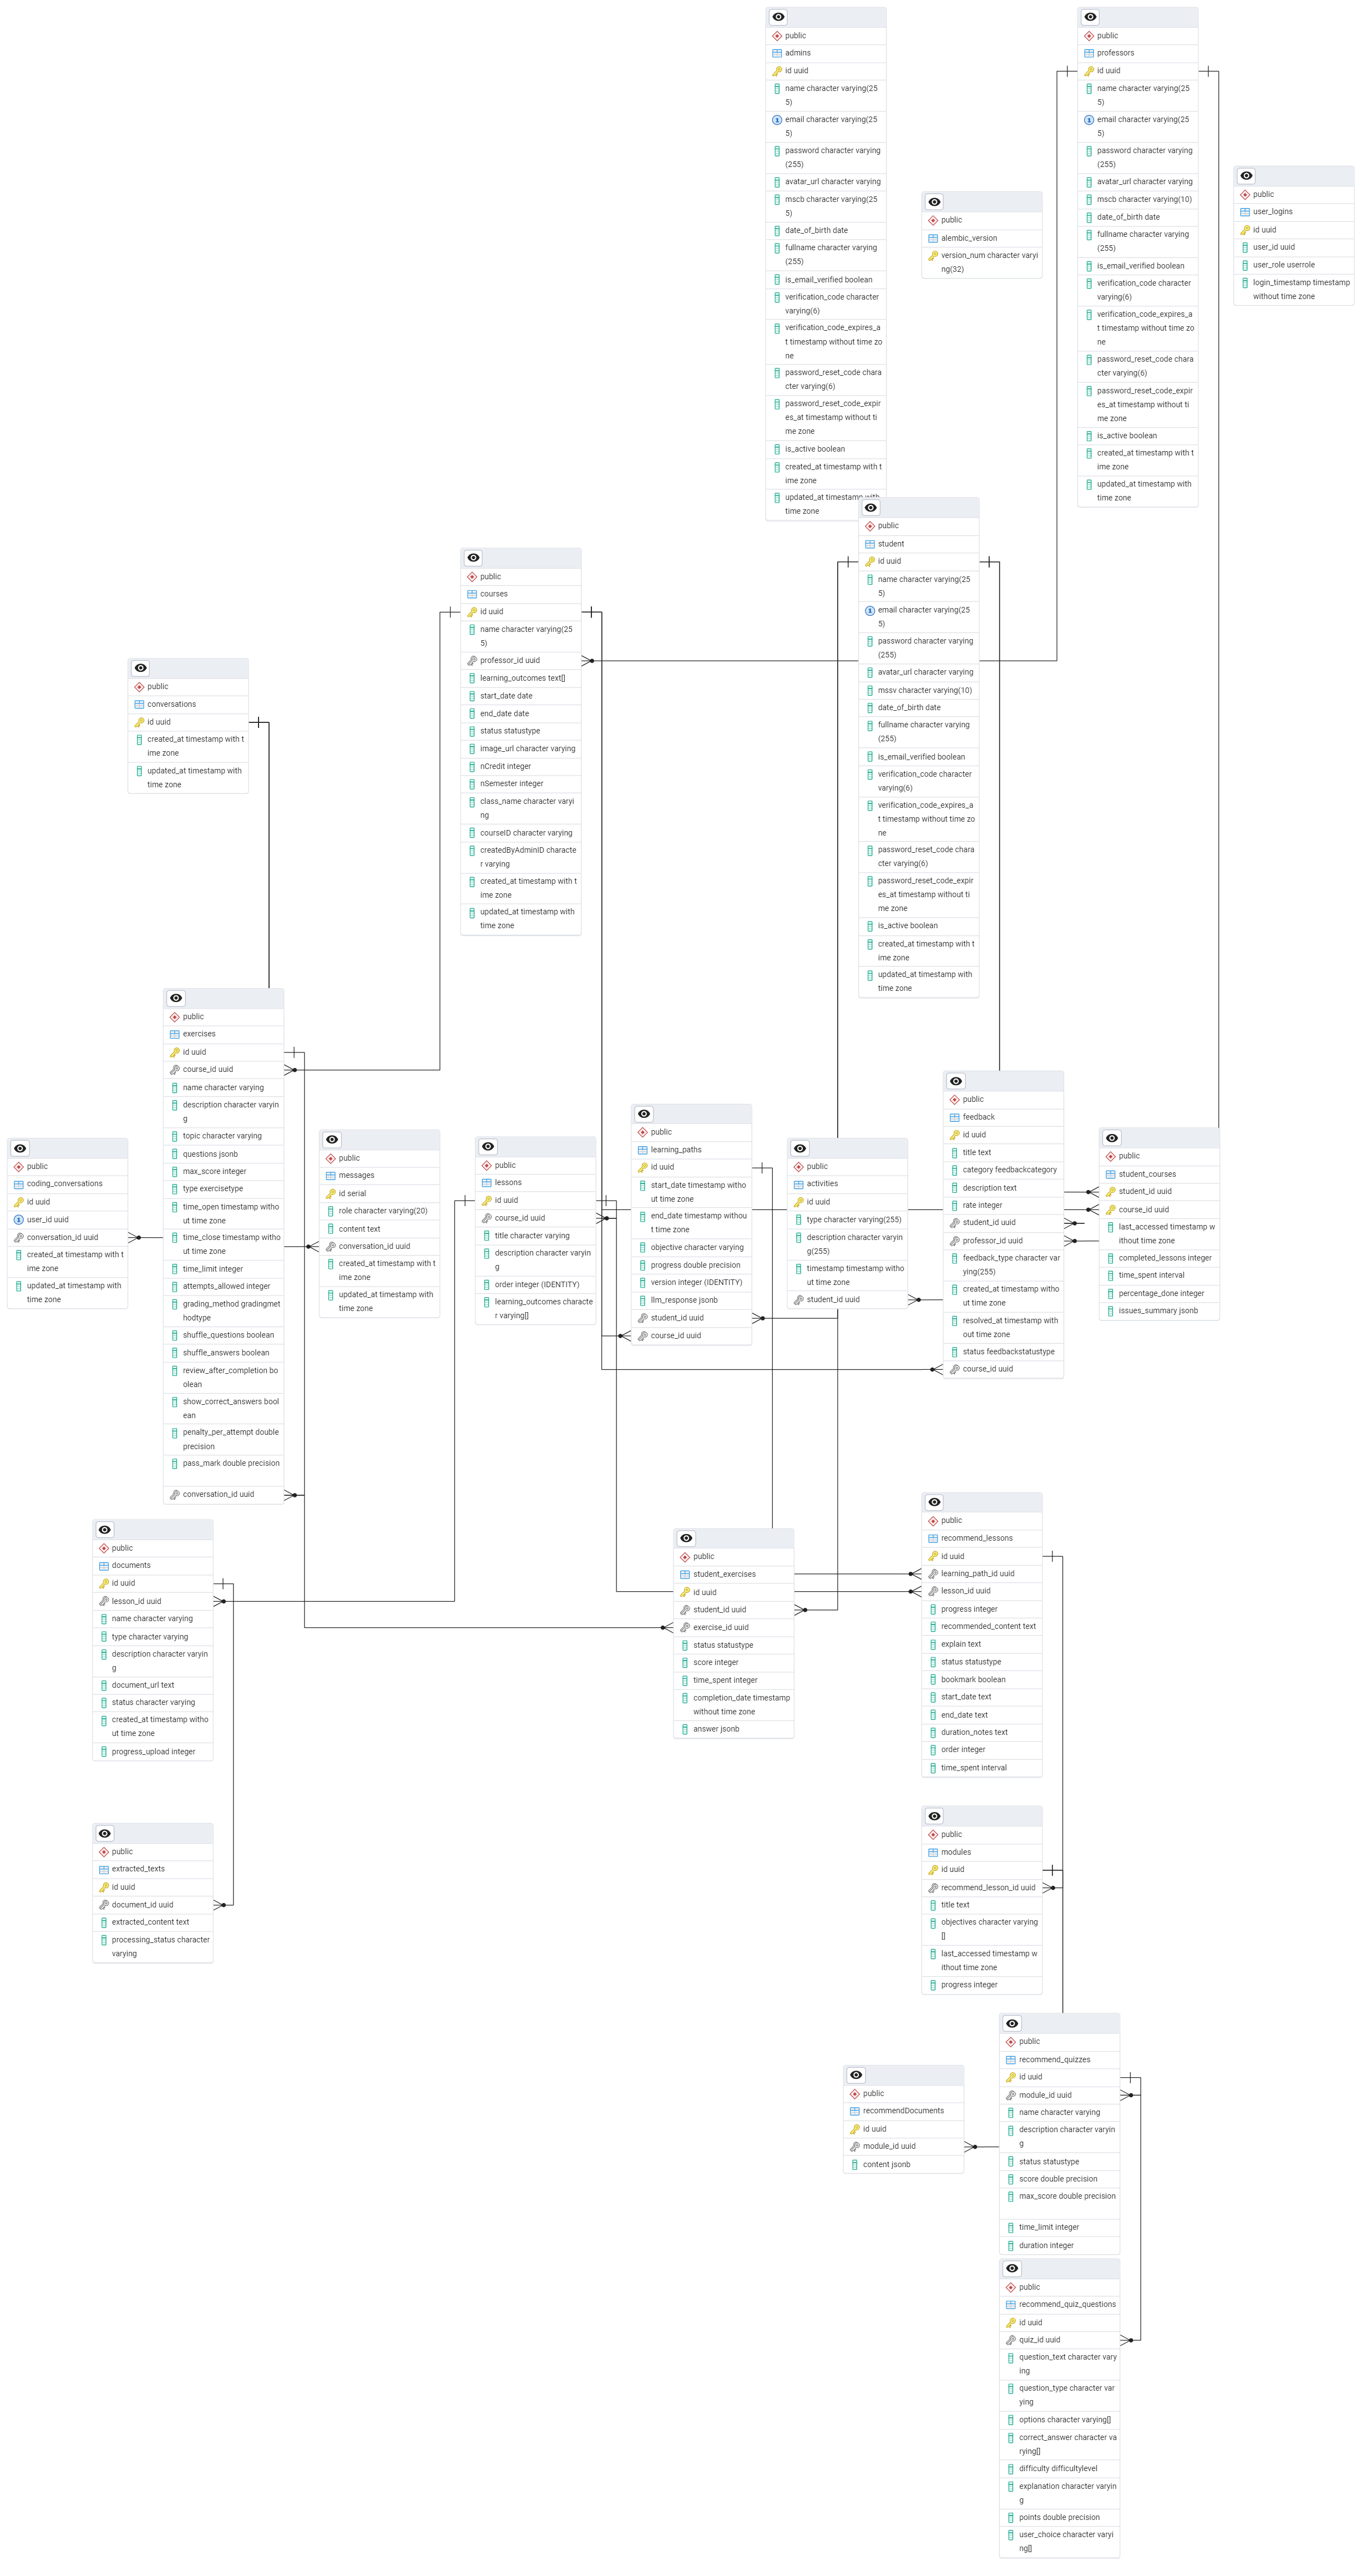
\includegraphics[width=0.6\linewidth]{images/ERD.png}
    \caption{Sơ đồ ERD của hệ thống}
    \label{fig:enter-label}
\end{figure}

\subsection{Tổng quan cấu trúc cơ sở dữ liệu}
Hệ thống được xây dựng trên nhiều bảng chính, chia thành các nhóm chức năng như sau:

\subsubsection{Nhóm người dùng (User Management)}
\begin{itemize}
    \item \textbf{professors}, \textbf{student}, \textbf{admins}: chứa thông tin cơ bản của người dùng theo 3 role như username, email, password,...
    \item \textbf{user\_login}\: bảng mở rộng lưu thông tin đăng nhập người dùng.
\end{itemize}

\subsubsection{Nhóm khóa học và tài liệu (Course Management)}
\begin{itemize}
    \item \textbf{courses}, \textbf{student\_courses}, \textbf{extracted\_text}: quản lý thông tin khóa học, tham gia khóa học và tài liệu học tập liên quan do giảng viên đăng tải.
    \item \textbf{lessons}, \textbf{documents}, \textbf{modules}: quản lý bài học và các nội dung bài học liên quan.
    \item \textbf{learning\_paths}, \textbf{recommend\_lessons}, \textbf{recommend\_documents}: quản lý các bài kiểm tra, bài tập và câu hỏi liên quan đến khóa học.
\end{itemize}

\subsubsection{Nhóm câu hỏi và bài kiểm tra (Assessment)}
\begin{itemize}
    \item \textbf{recommend\_quizzes}, \textbf{exercises}: chứa thông tin về các câu hỏi, loại câu hỏi, câu trả lời và kết quả bài kiểm tra của sinh viên trong các bài quiz được sinh ra theo từng bài học đề xuất.
\end{itemize}

\subsubsection{Nhóm tương tác và phản hồi (Interaction)}
\begin{itemize}
    \item  \textbf{feedbacks}, \textbf{activities}: quản lý tương tác giữa sinh viên và giảng viên, người dùng và hệ thống, và các hoạt động của người dùng.
\end{itemize}

\subsubsection{Nhóm bài tập Code Exercises}
\begin{itemize}
    \item \textbf{conversations}, \textbf{messages}, \textbf{coding\_conversations}: ghi nhận nhật ký hoạt động, cài đặt hệ thống và quản lý phiên làm việc.
\end{itemize}

\subsection{Mối quan hệ giữa các bảng}
Các bảng trong hệ thống có mối quan hệ nhiều-nhiều và một-nhiều, với các khóa ngoại được thể hiện rõ trong sơ đồ:
\begin{itemize}
    \item Một người dùng có thể tham gia nhiều khóa học thông qua bảng \texttt{student\_courses}.
    \item Một khóa học có thể có nhiều bài học, bài kiểm tra và tài liệu.
    \item Bài kiểm tra có thể bao gồm nhiều câu hỏi và mỗi câu hỏi có nhiều đáp án.
    \item Người dùng có thể đưa ra phản hồi và nhận thông báo từ hệ thống.
    \item Một sinh viên đối với một khóa học có thể có nhiều lộ trình học khác nhau. 
    \item Một lộ trình học có thể có nhiều bài học và tài liệu khác nhau.
    \item Một bài học có thể có nhiều module nhỏ và nội dung khác nhau.
    \item Một module có thể có nhiều bài quiz hoặc code exercises khác nhau (do sinh viên tùy chọn sinh ra)
\end{itemize}

\subsection{Kết luận}
Sơ đồ ERD này cung cấp một cái nhìn toàn diện về kiến trúc cơ sở dữ liệu của hệ thống. Cấu trúc được tổ chức hợp lý, cho phép dễ dàng mở rộng và tích hợp thêm các chức năng mới như AI hỗ trợ học tập, phân tích dữ liệu học viên, và hơn thế nữa.

\chapter{Giao diện người dùng}
% \section{Admin}
\subsection{Hoàn thiện Dashboard}
\begin{figure}[H]
    \centering
    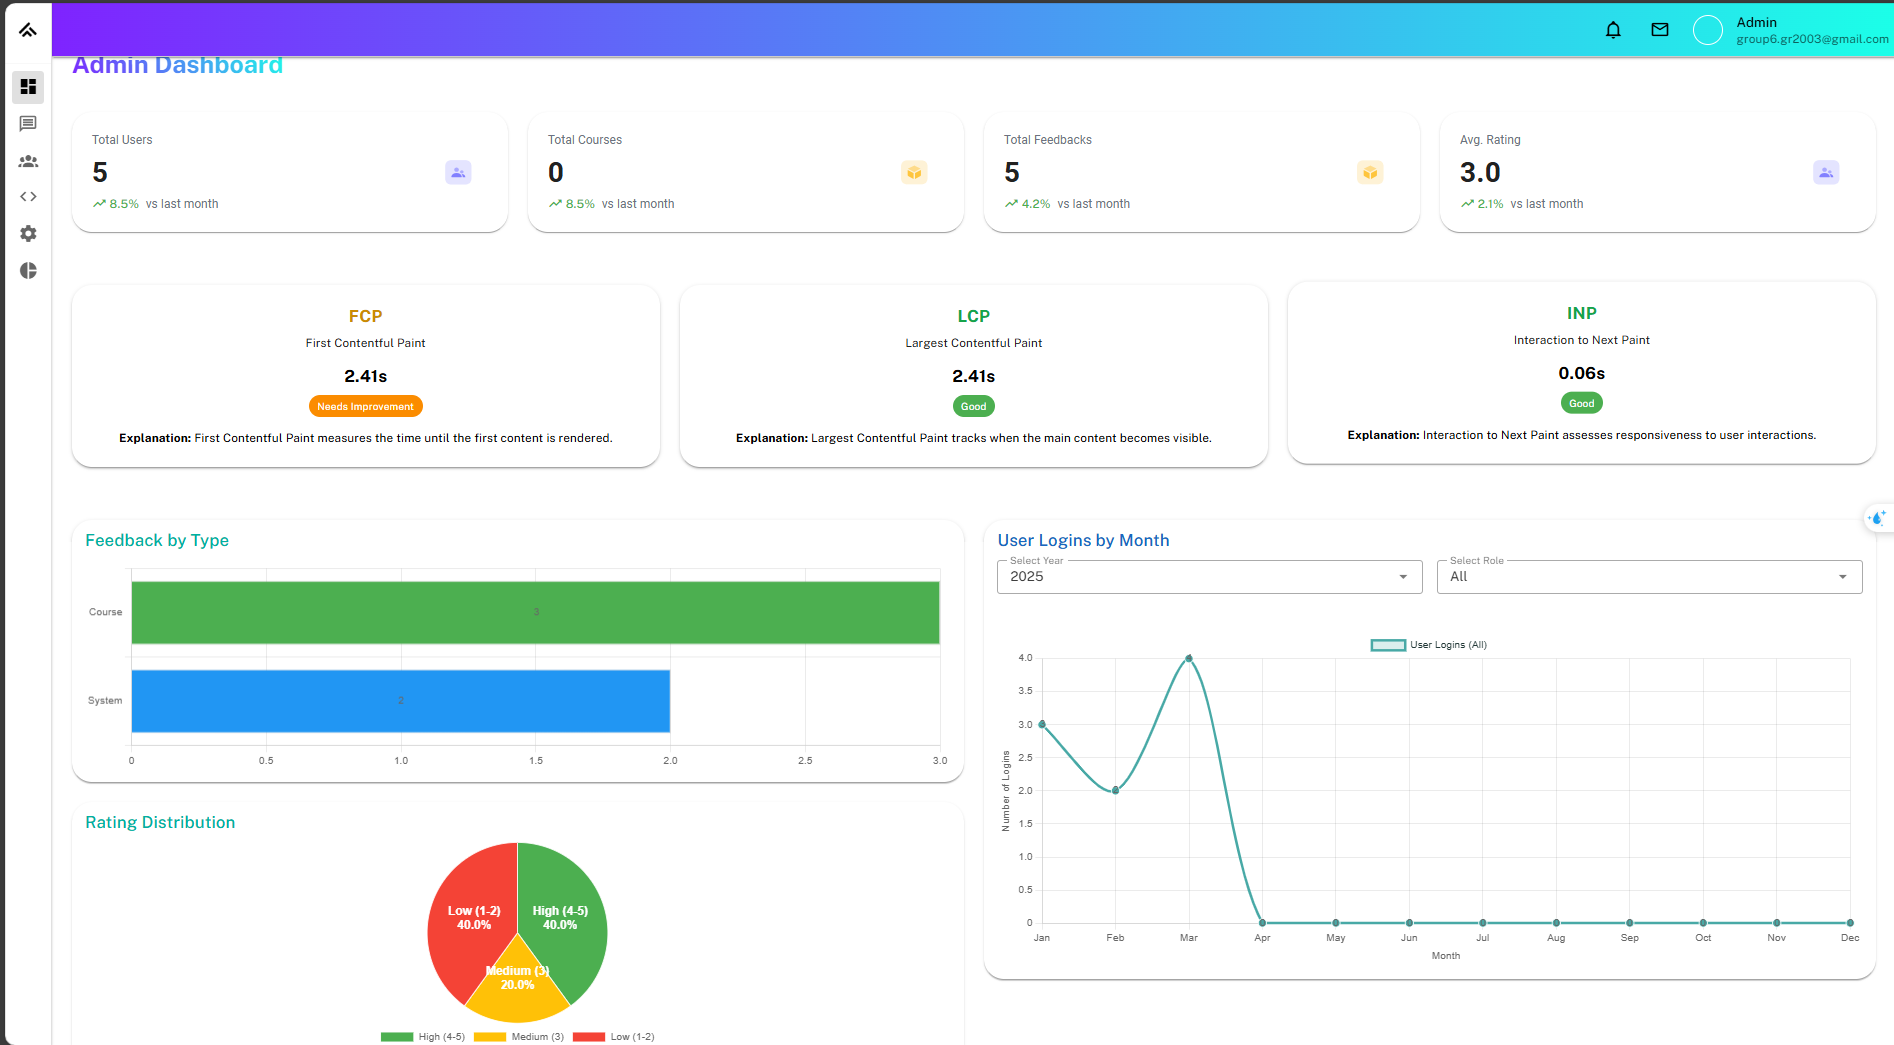
\includegraphics[width=0.8\linewidth]{images/admin_dashboard.png}
    \caption{Dashboard Admin}
    \label{fig:enter-label}
\end{figure}
Dashboard Admin, trang này như bảng điều khiển trung tâm để quản trị viên giám sát hệ thống. Nó hiển thị nổi bật các số liệu thống kê chính như:

\begin{itemize}
    \item Tổng số phản hồi gửi bởi người dùng.
    \item Tổng số người dùng đã đăng ký (bao gồm sinh viên, giáo viên và quản trị viên).
    \item Tổng số khóa học được cung cấp.
\end{itemize}

Các số liệu này cung cấp một cái nhìn tổng quan về hoạt động và mức độ tương tác của hệ thống. Dashboard tích hợp thêm biểu đồ để minh họa xu hướng theo thời gian, chẳng hạn như feedback hàng tuần hoặc sự tăng trưởng người dùng. 
\subsection{Quản lí các khóa học}
\begin{figure}[H]
    \centering
    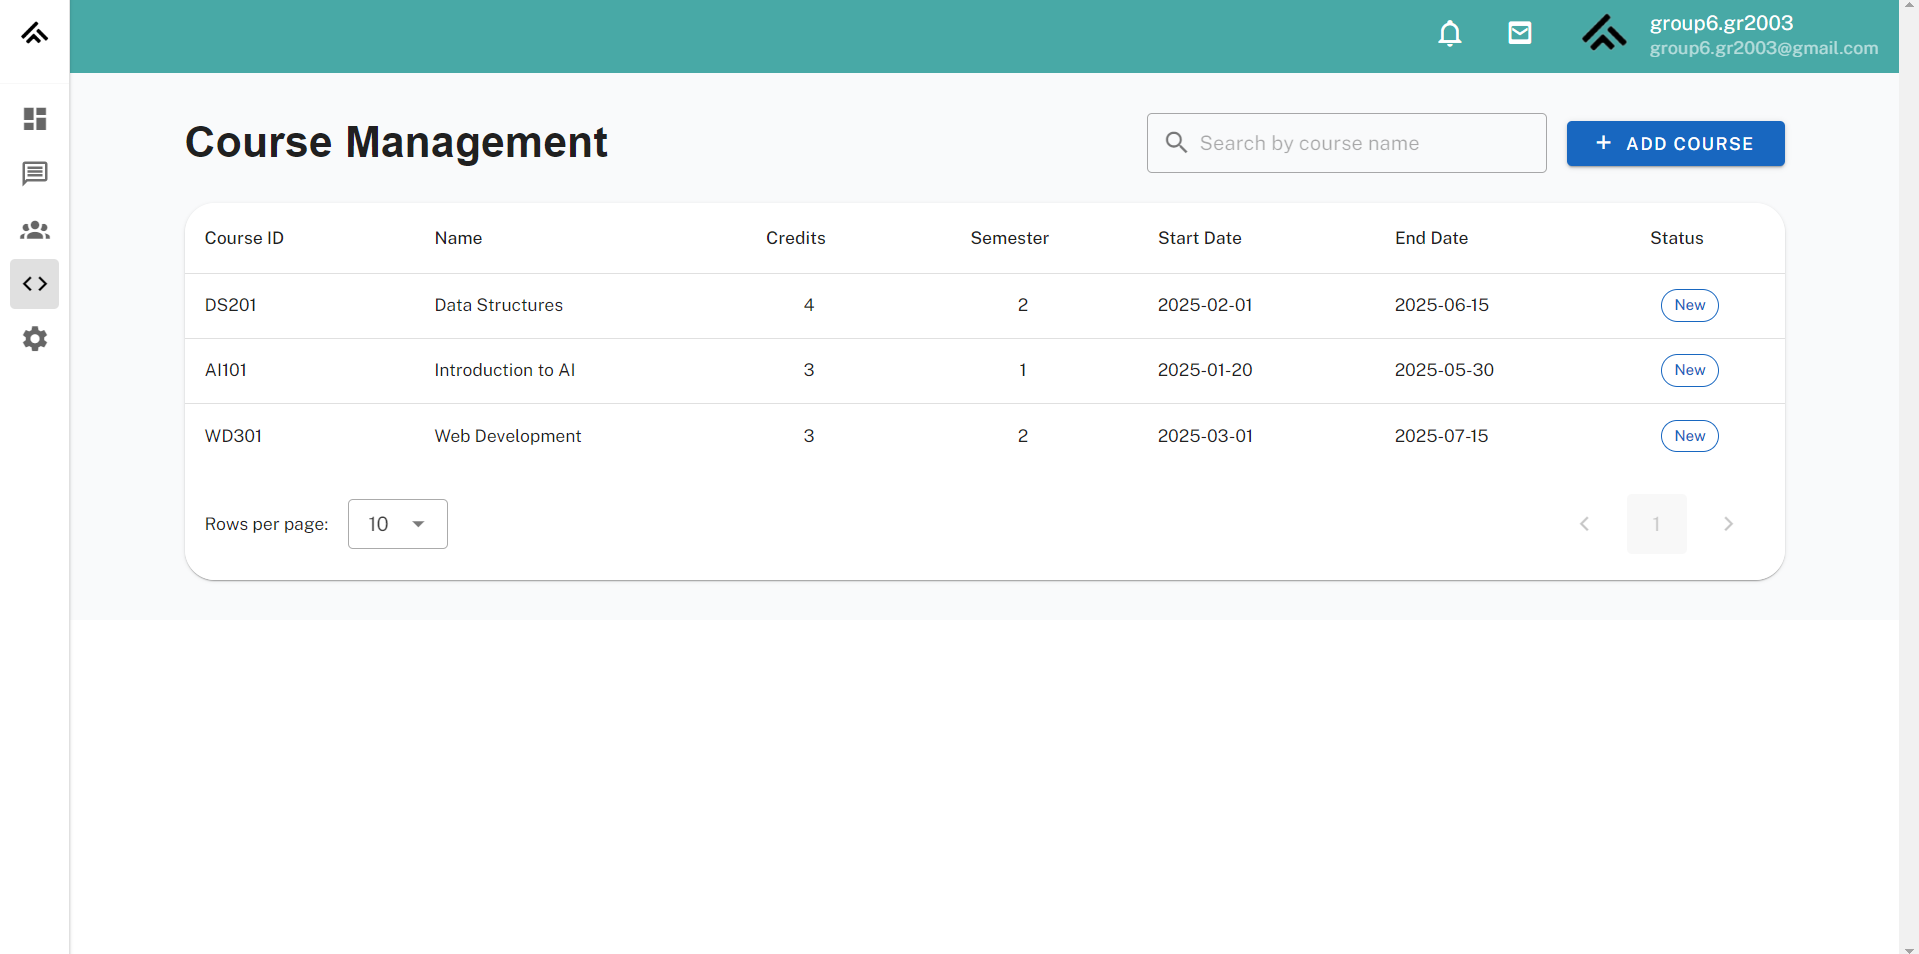
\includegraphics[width=0.8\linewidth]{images/admin_course_management.png}
    \caption{Quản lí danh sách khóa học của hệ thống}
    \label{fig:enter-label}
\end{figure}
Giao diện cung cấp một danh sách các khóa học với các cột chi tiết như:
\begin{itemize}
    \item Tiêu đề khóa học.
    \item Giáo viên, sinh viên được chỉ định.
    \item Số tín chỉ, học kì.
\end{itemize}

Quản trị viên có thể:
\begin{itemize}
    \item Chỉnh sửa chi tiết khóa học.
    \item Thêm khóa học mới.
    \item Xóa các khóa học.
\end{itemize}

\subsection{Thêm khóa học}
\begin{figure}[H]
    \centering
    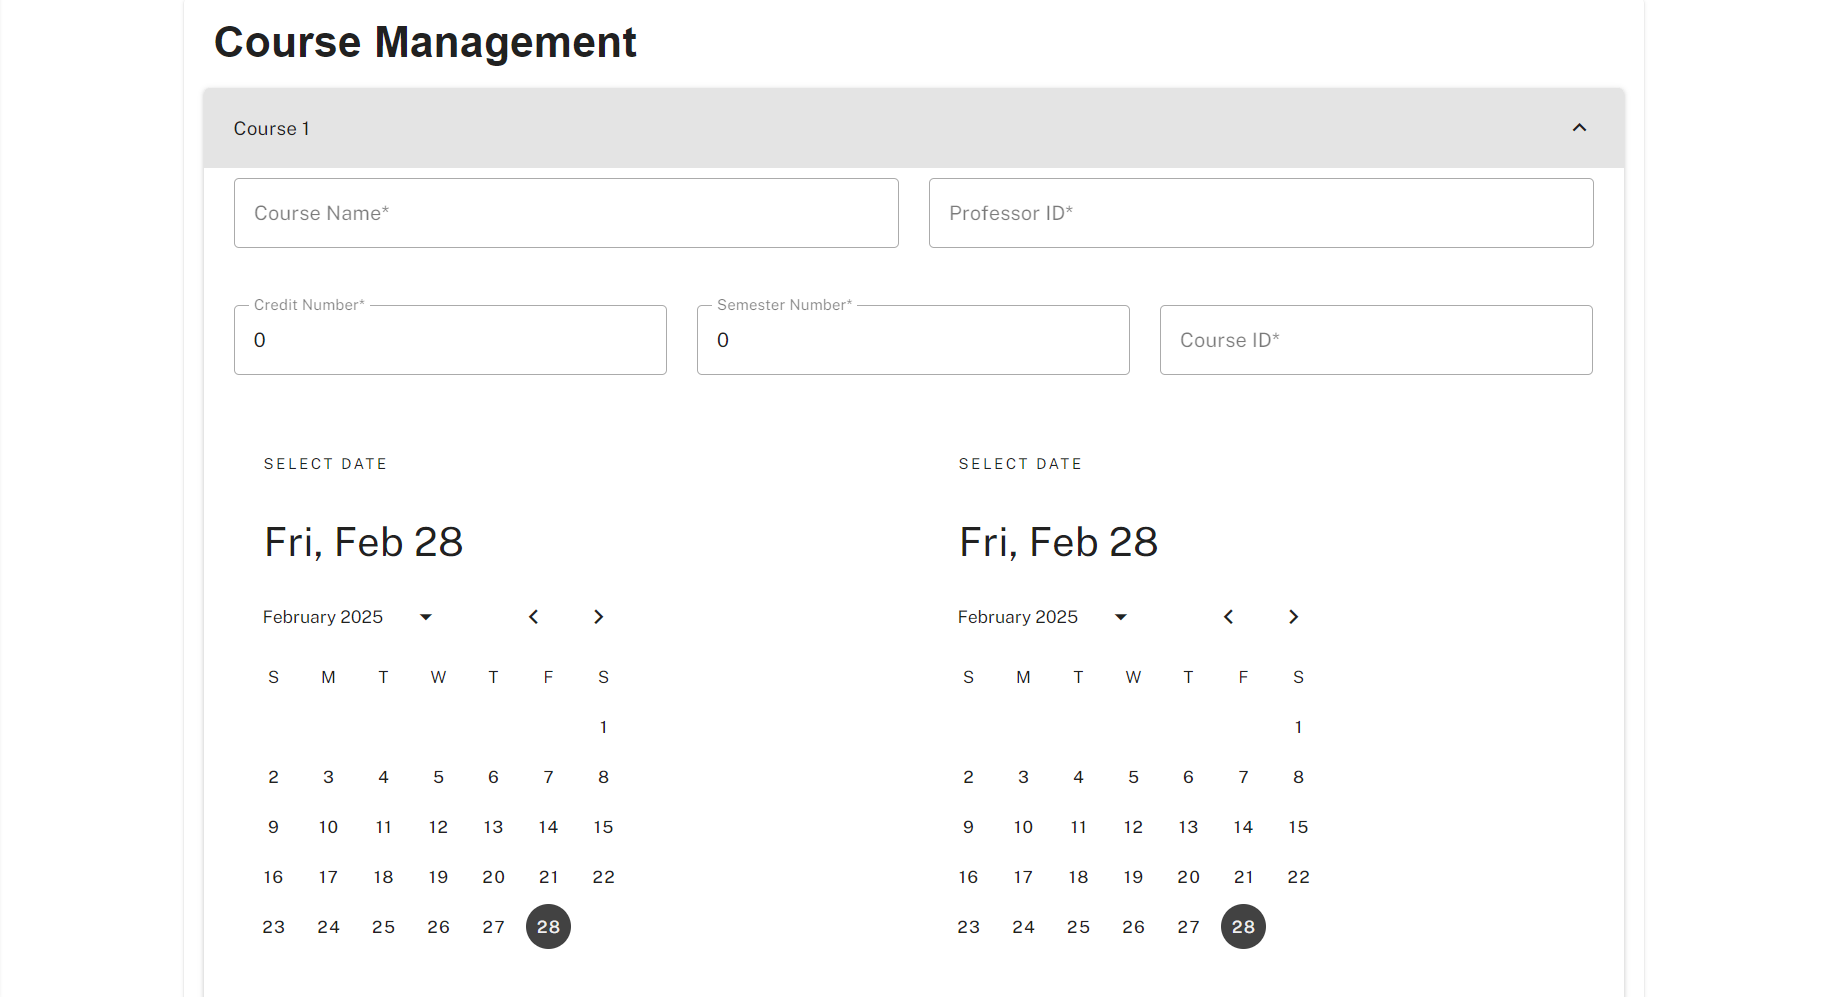
\includegraphics[width=0.8\linewidth]{images/admin_add_detail_course.png}
    \caption{Thông tin chi tiết khi thêm một khóa học}
    \label{fig:enter-label}
\end{figure}
Modal thêm khóa học bao gồm;
\begin{itemize}
    \item Tên khóa học: Mã định danh duy nhất.
    \item Mô tả khóa học: Tóm tắt mục tiêu và nội dung.
    \item Chỉ định giáo viên: ID của giáo viên phụ trách.
    \item Số tín chỉ, số học kì, thời gian khóa học
    \item Danh sách sinh viên
\end{itemize}
\begin{figure}[H]
    \centering
    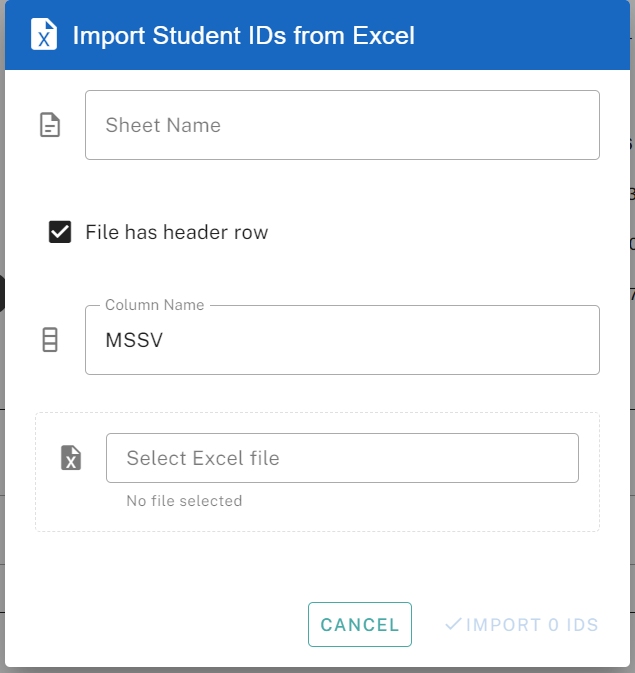
\includegraphics[width=0.6\linewidth]{images/admin_import_student_in_course.png}
    \caption{Thêm danh sách sinh viên vào khóa học}
    \label{fig:enter-label}
\end{figure}
Quá trình ghi danh sinh viên vào khóa học bằng cách nhập mã số từ tệp Excel. Tính năng này tối ưu hóa hiệu quả, đặc biệt với nhóm lớn. Giao diện cho phép:
\begin{itemize}
    \item Tải lên bảng Excel chứa mã số sinh viên (MSSV), tên, và có thể thêm email.
    \item Xác nhận tên sheet hoặc hàng tiêu đề để trích xuất dữ liệu chính xác.
\end{itemize}
So với nhập thủ công, quá trình này tiết kiệm thời gian và công sức, lý tưởng cho ghi danh hàng loạt vào đầu học kỳ hoặc chương trình đào tạo.
\begin{figure}[H]
    \centering
    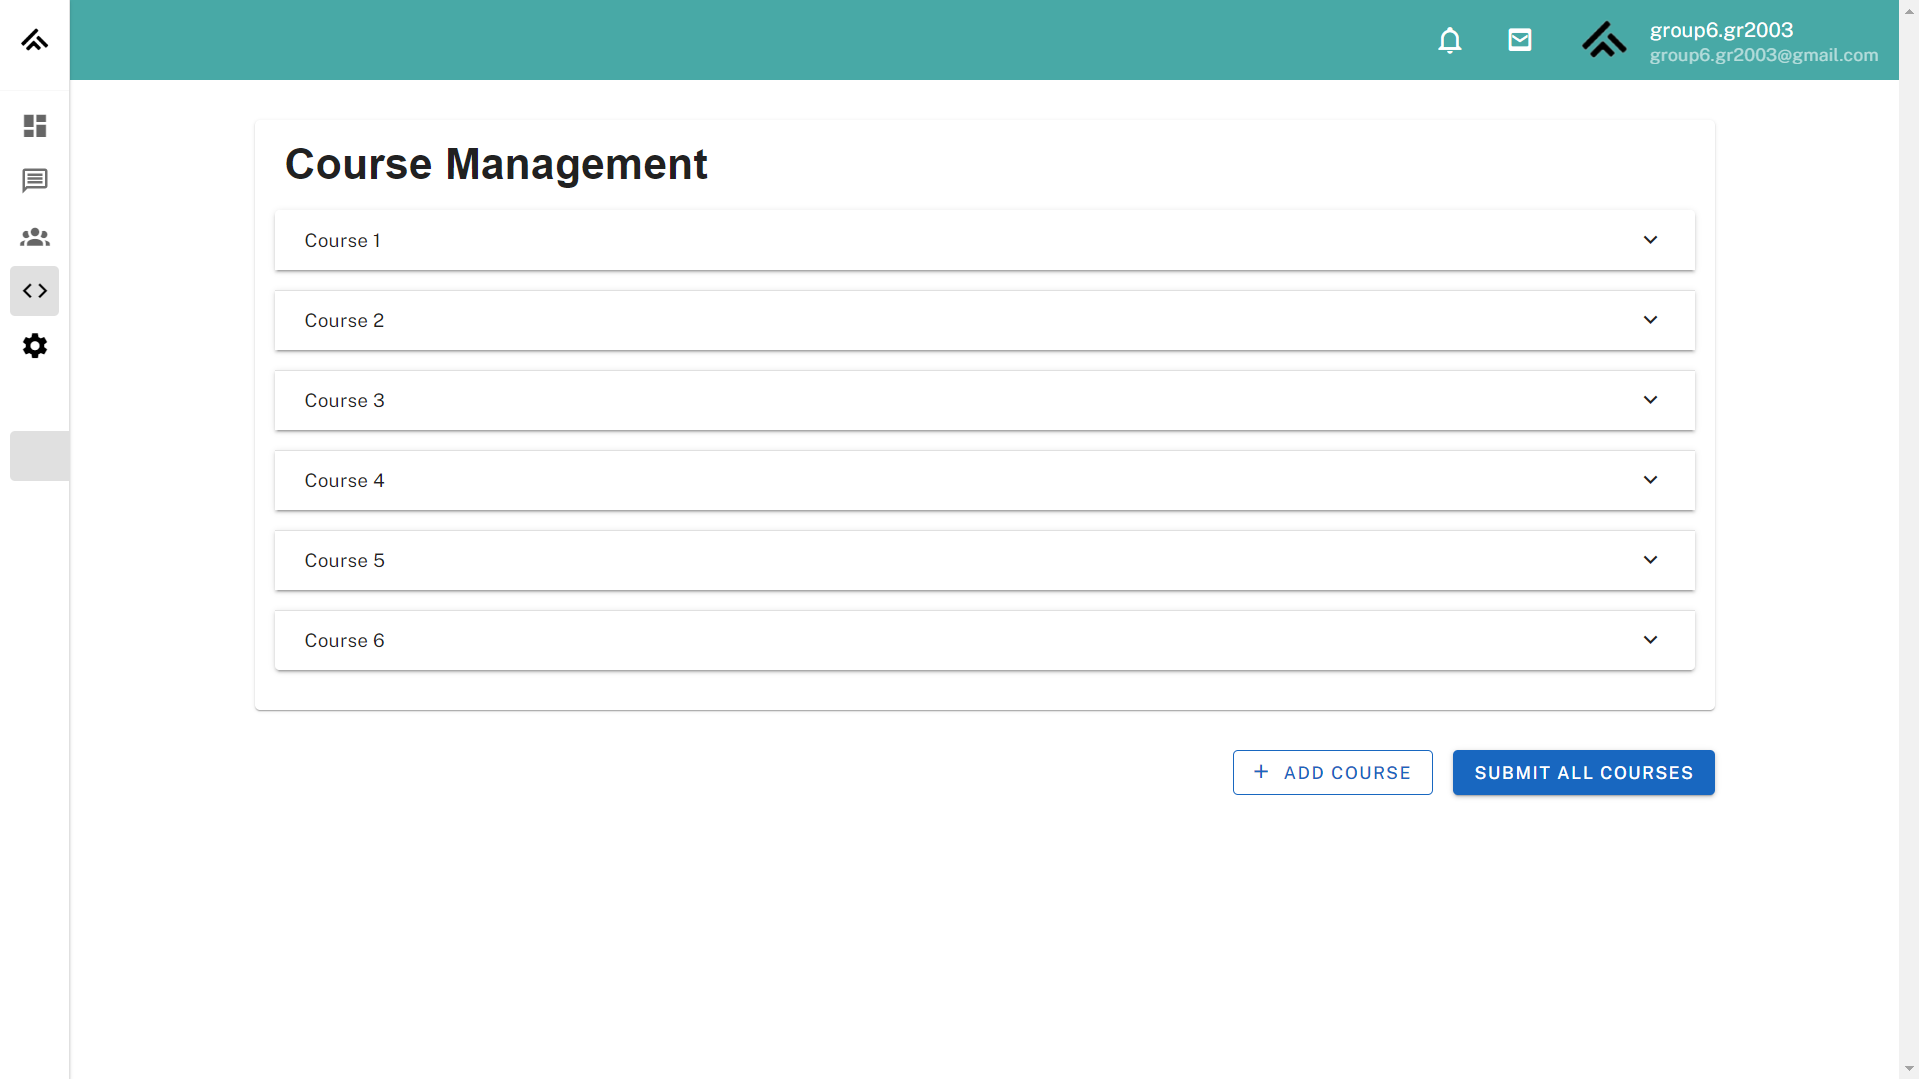
\includegraphics[width=0.6\linewidth]{images/admin_add_courses.png}
    \caption{Thêm nhiều khóa học}
    \label{fig:enter-label}
\end{figure}

Admin có thể thêm nhiều khóa học cùng một lúc.
\subsection{Thêm người dùng}
\begin{figure}[H]
    \centering
    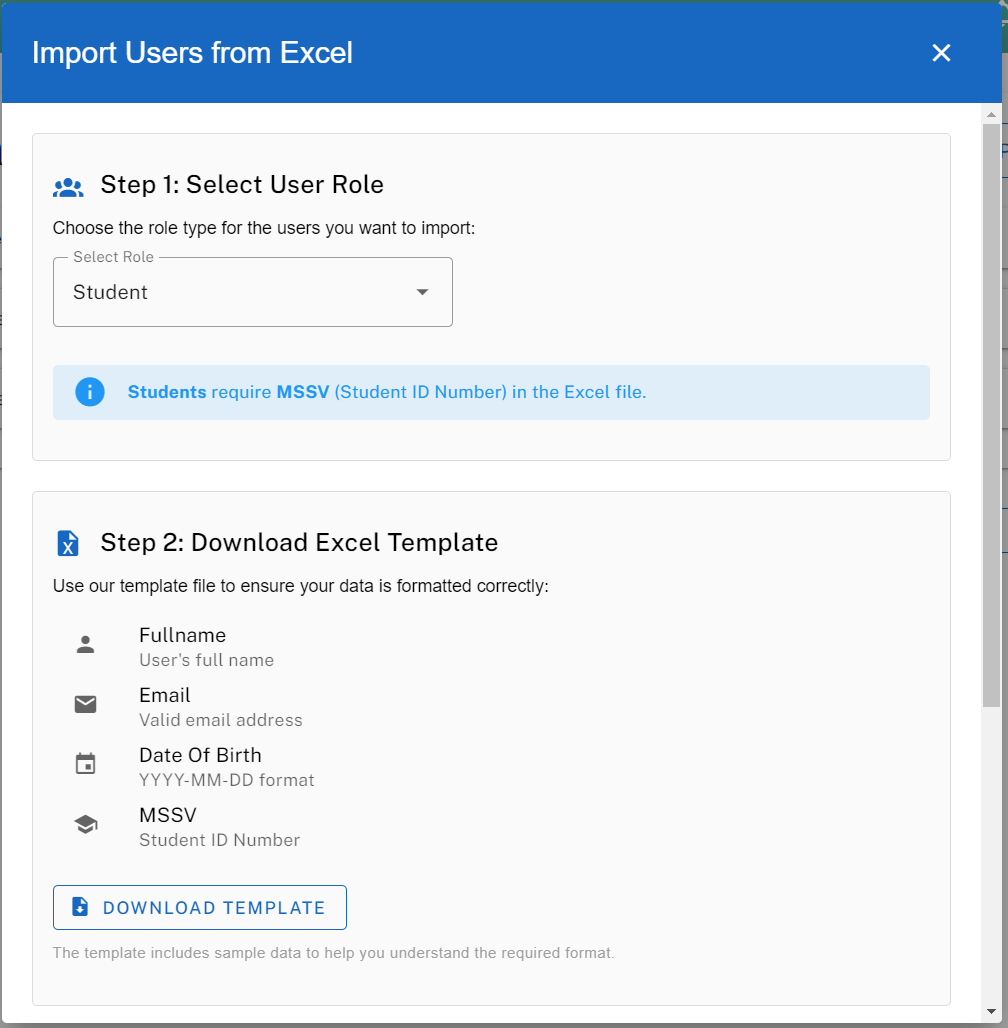
\includegraphics[width=0.6\linewidth]{images/admin_add_user_1.png}
    \caption{Thêm người dùng vào hệ thống }
    \label{fig:enter-label}
\end{figure}
\begin{figure}[H]
    \centering
    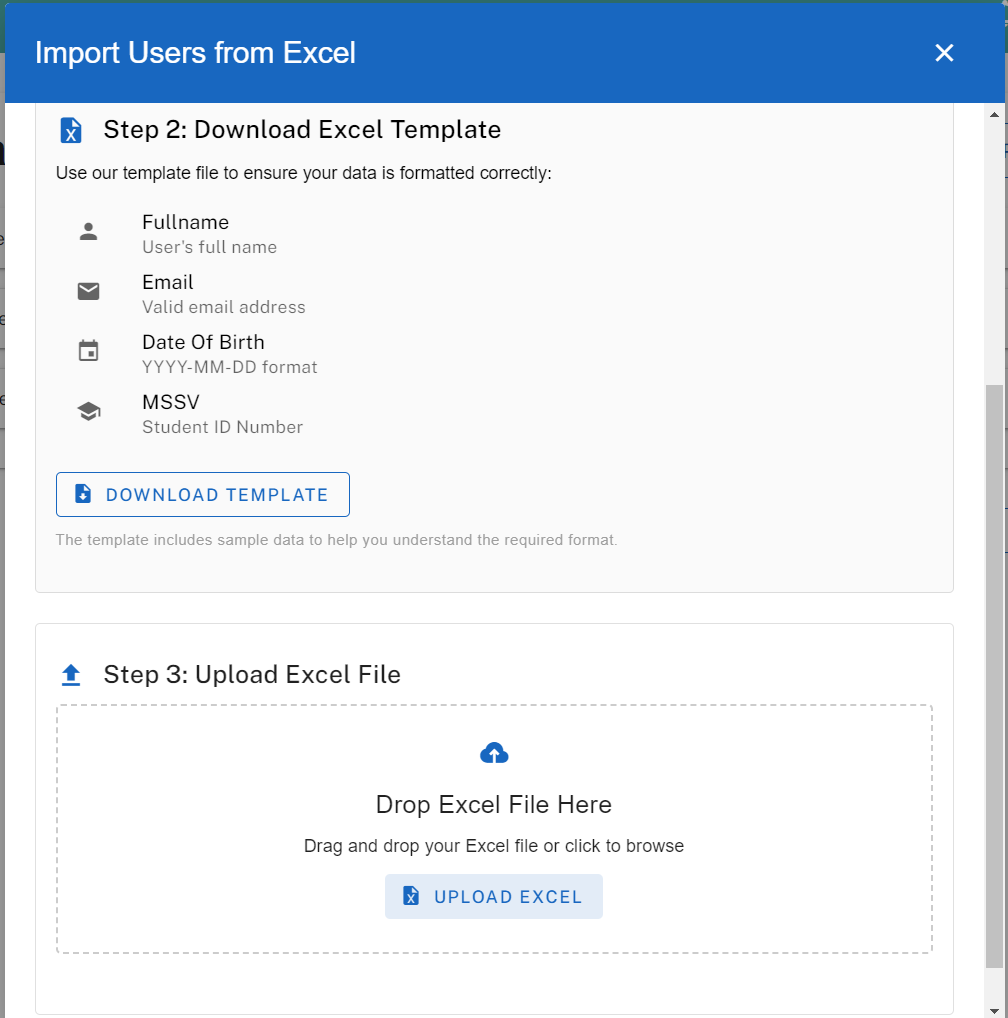
\includegraphics[width=0.6\linewidth]{images/admin_add_user_2.png}
    \caption{Caption}
    \label{fig:enter-label}
\end{figure}
Giao diện thêm người dùng mới (sinh viên, giáo viên, hoặc quản trị viên) vào nền tảng. Quản trị viên có thể:
\begin{itemize}
    \item Nhập dữ liệu từ mẫu Excel với thông tin như tên, mã số (MSSV), email, và vai trò.
    \item Cài đặt quyền theo vai trò (ví dụ: giáo viên tạo khóa học, sinh viên chỉ học).
\end{itemize}
\section{Code Area}
\subsection{Sử dụng Judge0 API}
\begin{itemize}
    \item Judge0 API là một hệ thống thực thi mã nguồn trực tuyến mã nguồn mở tiên tiến, được thiết kế để mạnh mẽ và có khả năng mở rộng. Đây là một công cụ cho phép thực hiện việc chạy mã nguồn trong nhiều ngôn ngữ lập trình khác nhau
    \item Điểm nổi bật của Judge0 là tính linh hoạt và khả năng tùy chỉnh. Judge0 API cho phép tùy chọn biên dịch, thêm đối số dòng lệnh, hoặc đặt giới hạn về thời gian và bộ nhớ khi thực thi mã nguồn. Điều này đặc biệt quan trọng nếu bạn dùng Judge0 trong các tác vụ đòi hỏi hiệu suất cao.
    \item Judge0 API hỗ trợ hơn 60 ngôn ngữ lập trình, từ những ngôn ngữ phổ biến mà bạn có thể đã sử dụng đến những ngôn ngữ ít gặp hơn.
\end{itemize}


\subsection{Thiết kế chức năng cho student làm bài tập: code}
\begin{figure}[H]
    \centering
    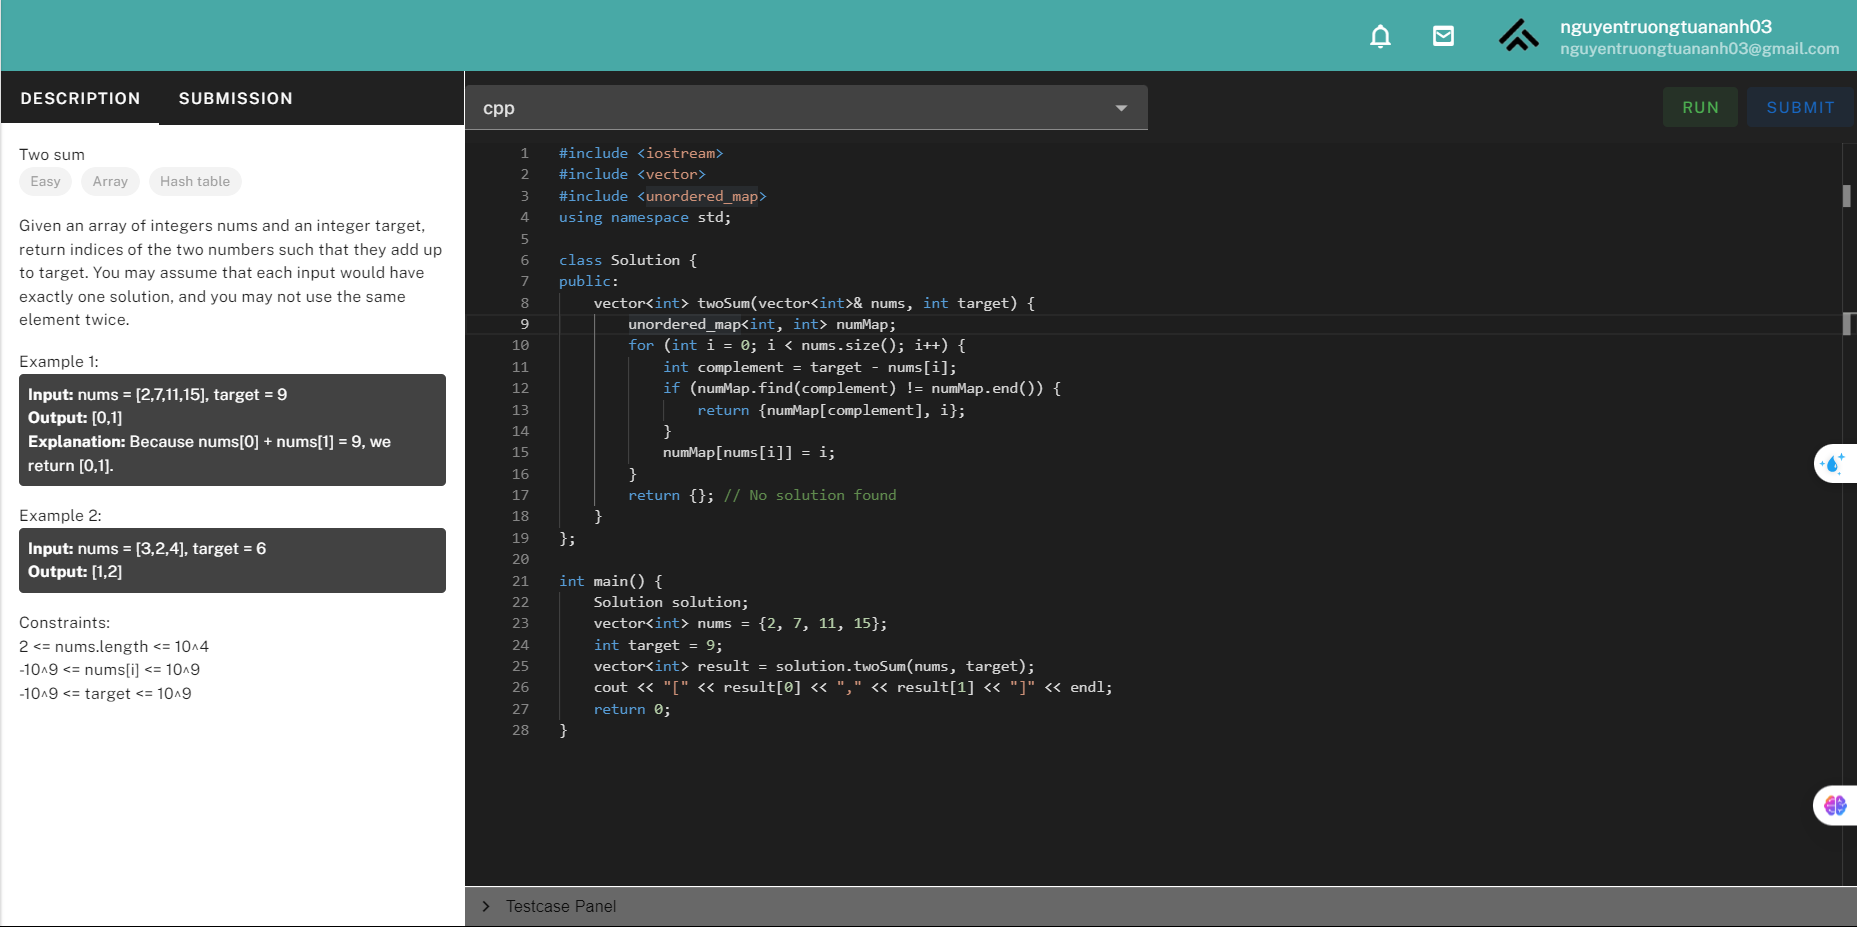
\includegraphics[width=0.8\linewidth]{images/code_area.png}
    \caption{Khu vực làm bài tập code}
    \label{fig:enter-label}
\end{figure}
Sinh viên có thể chọn ngôn ngữ lập trình, xem hướng dẫn, và truy cập mẫu đầu vào/đầu ra. Thiết lập này mô phỏng công cụ phát triển chuyên nghiệp, kết nối lý thuyết và thực hành. Tích hợp API Judge0 cung cấp đánh giá mã tự động, mang lại phản hồi tức thì để cải thiện kỹ năng học tập.
\begin{figure}[H]
    \centering
    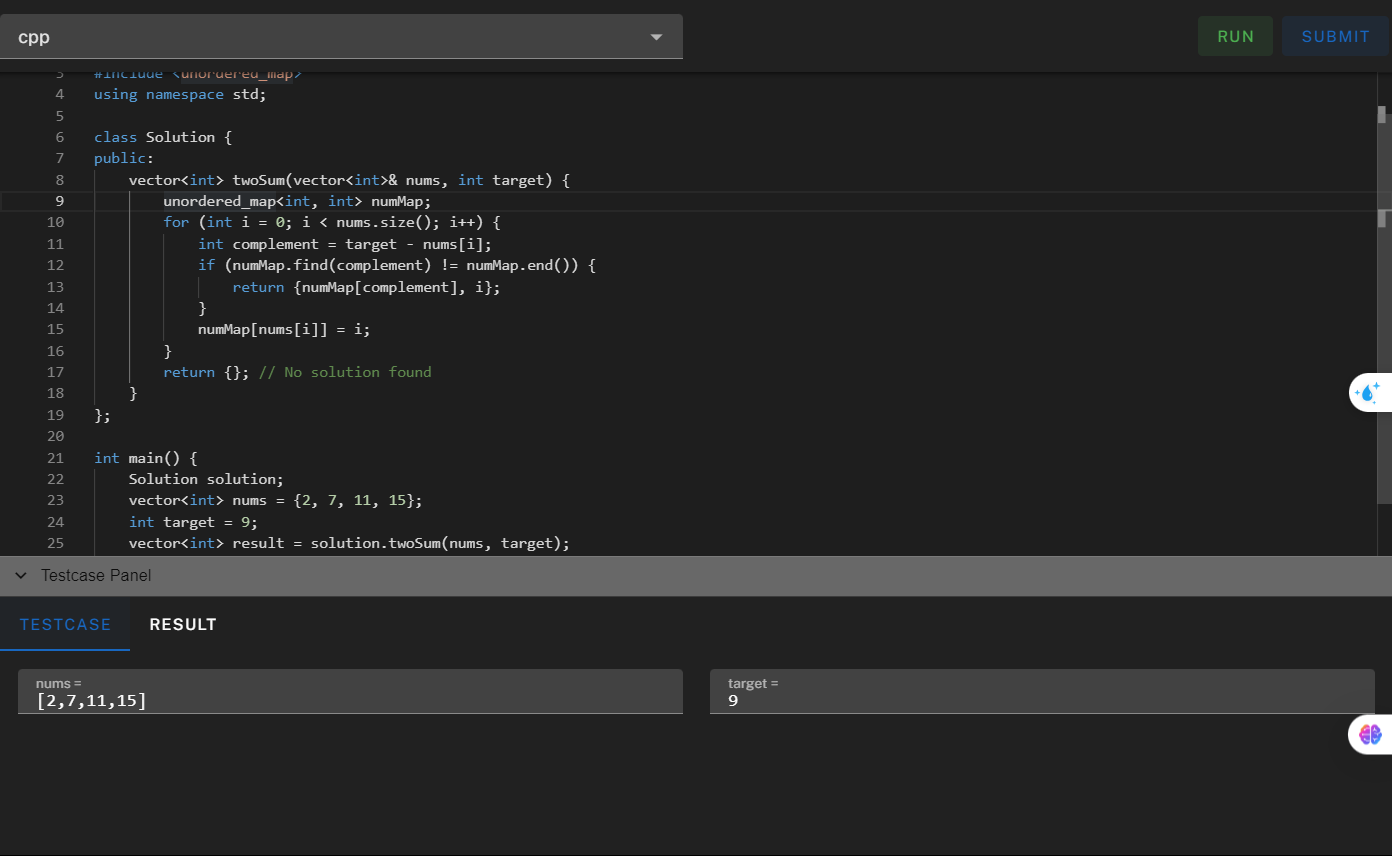
\includegraphics[width=0.8\linewidth]{images/code_testcase.png}
    \caption{Testcase bài tập}
    \label{fig:enter-label}
\end{figure}
Gaio diện hiển thị các testcase cho bài tập lập trình, cần thiết để đánh giá bài code của sinh viên. Mỗi trường hợp bao gồm:
\begin{itemize}
    \item Đầu vào cụ thể và đầu ra dự kiến.
    \item Một số hiển thị để hướng dẫn, một số ẩn để kiểm tra toàn diện.
\end{itemize}

\begin{figure}[H]
    \centering
    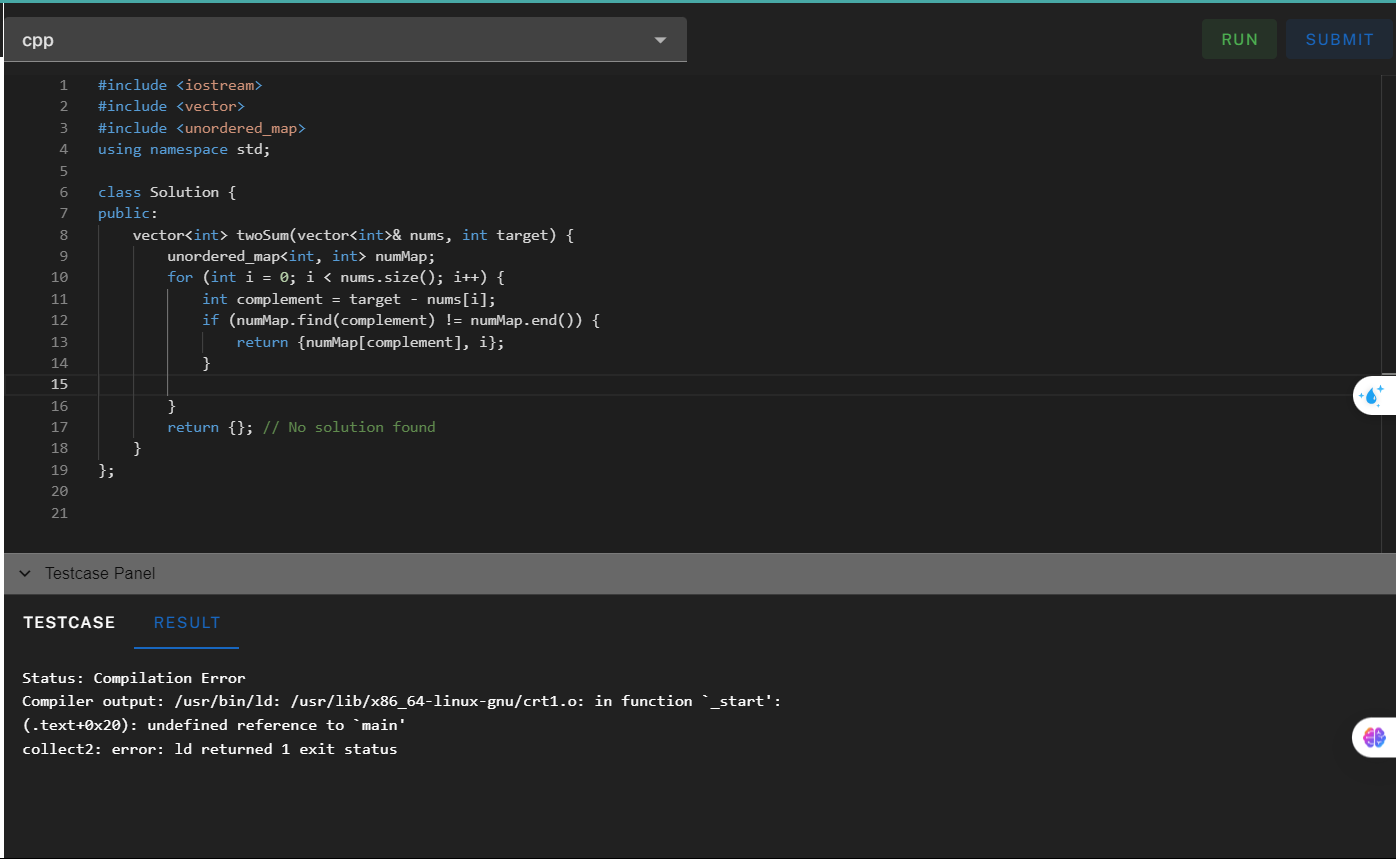
\includegraphics[width=0.8\linewidth]{images/code_run_error.png}
    \caption{Thông báo kết quả khi code chạy lỗi}
    \label{fig:enter-label}
\end{figure}
Kết quả thông báo lỗi khi đoạn code sinh viên lỗi
\begin{itemize}
    \item Loại lỗi: Cú pháp, thời gian chạy, v.v.
    \item Số dòng: Vị trí lỗi.
    \item Phản hồi chi tiết giúp sinh viên xác định sai lầm, hiểu nguyên nhân, và học hỏi.
\end{itemize}
\begin{figure}[H]
    \centering
    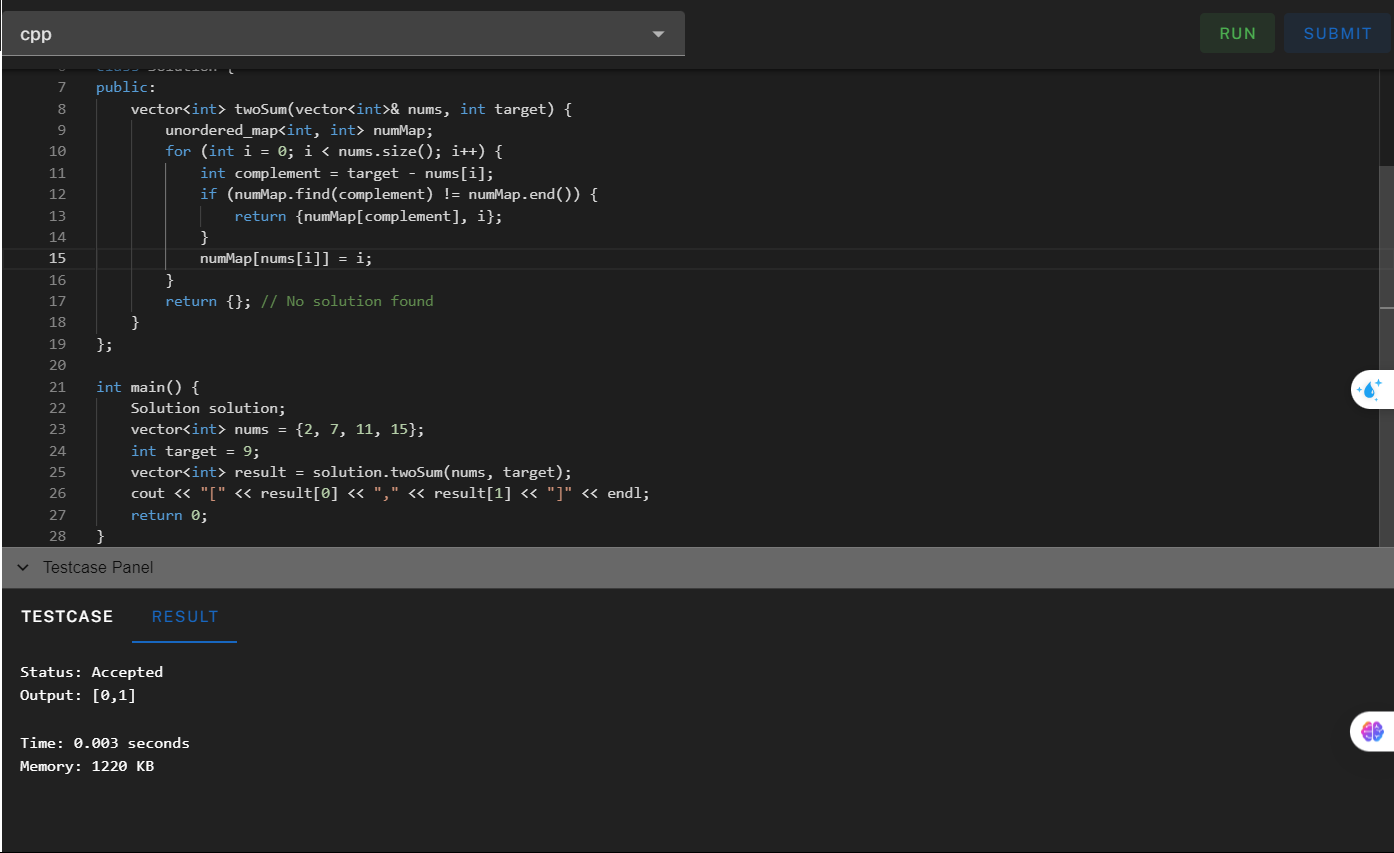
\includegraphics[width=0.8\linewidth]{images/code_run_success.png}
    \caption{Thông báo kết quả khi code chạy thành công}
    \label{fig:enter-label}
\end{figure}
Kết quả thông báo khi đoạn code sinh viên chạy thành công
\begin{itemize}
    \item Số trường hợp kiểm thử đã qua.
    \item Chỉ số hiệu suất (thời gian thực thi, bộ nhớ).
    \item Thông báo này củng cố tích cực, cung cấp cái nhìn về hiệu quả mã.
\end{itemize}
% \chapter{Triển khai và phát triển}
% 
Trong suốt quá trình phát triển, nhóm dự án đã thực hiện nhiều nhiệm vụ quan trọng để đảm bảo hệ thống học tập trực tuyến được triển khai thành công, đáp ứng yêu cầu và tối ưu hóa trải nghiệm người dùng. Các nhiệm vụ được phân chia theo tuần và người đảm nhiệm, từ việc phát triển các tính năng cơ bản đến việc tích hợp các công nghệ tiên tiến như mô hình ngôn ngữ lớn (LLM) và triển khai hệ thống.

\section{Giai đoạn 1: Phát triển API và Giao diện cơ bản (Tuần 1-3)}

\begin{itemize}[label=-]
    \item Trong tuần đầu tiên, nhóm đã bắt tay vào phát triển các tính năng cốt lõi của hệ thống. 
    \item \textbf{\textit{Phạm Thi}} đảm nhận nhiệm vụ phát triển API cho chức năng đăng nhập và đăng ký, đảm bảo tính bảo mật cho hệ thống thông qua mã hóa mật khẩu và xác thực người dùng. Giao diện UI cho trang đăng nhập và đăng ký cũng được thiết kế đơn giản và dễ sử dụng. Các trường hợp đặc biệt như mật khẩu sai hoặc tài khoản không tồn tại được kiểm tra kỹ lưỡng.
    \item \textbf{\textit{Tuấn Anh}} phụ trách thiết kế giao diện trang giới thiệu của hệ thống, cung cấp thông tin về các tính năng và cách thức hoạt động của hệ thống. Trang landing page này được kiểm tra kỹ lưỡng về tính tương thích và khả năng tương tác trên các nền tảng khác nhau.
    \item \textbf{\textit{Tuấn Anh}} đảm nhiệm việc phát triển API quản lý khóa học cho giảng viên, bao gồm các tính năng thêm, sửa và xóa khóa học, cũng như khả năng upload tài liệu cho từng bài học. Các trường hợp lỗi như tài liệu không đúng định dạng hoặc thiếu thông tin được xử lý rõ ràng.
\end{itemize}

\section{Giai đoạn 2: Quản lý Tiến độ Học tập và Tích hợp API (Tuần 4-6)}

\begin{itemize}[label=-]
    \item Trong tuần tiếp theo, nhóm tiếp tục phát triển các tính năng phục vụ giảng viên và sinh viên. 
    \item \textbf{\textit{Tuấn Anh}} đã hoàn thiện API và giao diện người dùng để giảng viên có thể theo dõi tiến độ học tập của sinh viên. Các tính năng lọc và phân loại học sinh theo tiến độ học tập cũng được thêm vào.
    \item \textbf{\textit{Phạm Thi}} phát triển API để lưu trữ và xử lý dữ liệu học tập của sinh viên, đảm bảo tính chính xác trong việc theo dõi tiến độ học tập. Các API này còn được tích hợp với các hệ thống khác để đồng bộ và cập nhật dữ liệu kịp thời.
    \item \textbf{\textit{Phạm Thi}} phát triển API cho quản lý người dùng (admin), cho phép quản trị viên có thể xem, thêm, sửa và xóa tài khoản của sinh viên và giảng viên. Đồng thời, các quyền truy cập và bảo mật thông tin người dùng cũng được thiết lập và kiểm tra.
\end{itemize}

\section{Giai đoạn 3: Tích hợp Mô hình Ngôn ngữ Lớn (LLM) và Tự động hóa (Tuần 7-10)}

\begin{itemize}[label=-]
    \item Nhóm tiếp tục triển khai các tính năng thông minh, đặc biệt là tích hợp mô hình ngôn ngữ lớn (LLM) để tạo các câu hỏi trắc nghiệm tự động và tài liệu ôn tập.
    \item \textbf{\textit{Tuấn Anh}} phụ trách phát triển API cho việc tạo câu hỏi trắc nghiệm và tài liệu học tập tự động từ nội dung bài giảng, đồng thời kiểm tra độ chính xác của các câu hỏi được tạo ra.
    \item \textbf{\textit{Phương Nam}} phát triển các module hỗ trợ lập trình, bao gồm gợi ý sửa lỗi (Code Hint Module), trợ giúp gỡ lỗi (Debugging Assistant), và giải thích mã nguồn (Explain Code Module). Những tính năng này giúp sinh viên nhận được hỗ trợ trực tiếp trong quá trình học lập trình, tối ưu hóa khả năng học tập.
    \item \textbf{\textit{Tuấn Anh}} phát triển API chấm điểm tự động cho câu trả lời của sinh viên, sử dụng LLM để phân tích và đánh giá các câu trả lời, đảm bảo tính chính xác và khách quan trong việc chấm điểm.
\end{itemize}


\chapter{Chi tiết cách thức hoạt động của một số tính năng chính}
\section{Giới thiệu}
Hệ thống học tập thông minh được thiết kế để hỗ trợ học sinh trong việc lập kế hoạch học tập và đánh giá tiến độ một cách hiệu quả. Với sự tích hợp của AI, hệ thống có khả năng phân tích dữ liệu học tập, tạo lộ trình cá nhân hóa và đưa ra các đánh giá chi tiết. Báo cáo này tập trung vào các chức năng chính như sinh ra lộ trình học tập, đánh giá kết quả học tập, và các tính năng bổ sung khác.

\section{Sinh ra lộ trình học tập}
Chức năng này chịu trách nhiệm tạo ra một lộ trình học tập cá nhân hóa dựa trên mục tiêu học tập của học sinh, nội dung khóa học và thời gian khả dụng. Quá trình được thực hiện qua ba giai đoạn chính:

\begin{enumerate}
    \item \textbf{Phân tích mục tiêu và thời gian}: Hàm \texttt{analyze\_goal\_and\_timeline} kiểm tra tính hợp lệ của mục tiêu (ví dụ: độ dài, tính liên quan) và xác định thời gian khả thi dựa trên ngày bắt đầu và kết thúc khóa học. Ví dụ mã nguồn:
    \begin{lstlisting}[language=Python]
async def analyze_goal_and_timeline(goal: str, course_start_date: datetime, ...):
    if len(goal) < 10:
        raise ApplicationException(message="Goal is too short...")
    prompt = f"..."
    response = chunking_manager.call_llm_api(prompt, ...)
    \end{lstlisting}

    \item \textbf{Lựa chọn bài học liên quan}: Hàm \texttt{select\_relevant\_lessons} lọc các bài học phù hợp với mục tiêu, sắp xếp theo thứ tự logic và điều chỉnh theo thời gian. AI được sử dụng để ưu tiên các bài học nền tảng nếu thời gian ngắn.

    \item \textbf{Tạo lộ trình chi tiết}: Hàm \texttt{generate\_detailed\_learning\_path} xây dựng lộ trình đầy đủ, bao gồm các bài học được đề xuất và phân bổ thời gian cụ thể. Kết quả được lưu vào cơ sở dữ liệu qua endpoint \texttt{/generate-learning-path}.
\end{enumerate}

Kết quả là một JSON chứa thông tin chi tiết về lộ trình, ví dụ:
\begin{lstlisting}[language=JSON]
{
    "learning_path_start_date": "2025-04-06",
    "recommend_lessons": [{"lesson_id": "123", "order": 1, ...}]
}
\end{lstlisting}

\section{Đánh giá kết quả học tập}
Chức năng này bao gồm hai phần phụ: theo dõi quá trình học tập và phân tích kết quả cuối cùng.

\subsection{Đánh giá quá trình học tập (Progress Tracking Assessment)}
Phần này sử dụng endpoint \texttt{/student/\{courseId\}/assessment} để đánh giá tiến độ học tập dựa trên phương pháp STAR (Situation, Task, Action, Result). Các bước thực hiện:
\begin{itemize}
    \item \textbf{Tạo prompt chuẩn}: Hàm \texttt{generate\_standard\_prompt} sinh ra một prompt chi tiết gửi đến AI, yêu cầu đánh giá dựa trên các tiêu chí: kiến thức lý thuyết, kỹ năng thực hành (hoặc kỹ năng thay thế), và sự nỗ lực.
    \item \textbf{Phân tích dữ liệu}: AI sử dụng dữ liệu bài học (progress, time\_spent) để đưa ra đánh giá theo Rubric chuẩn, với các mức: Excellent, Good, Average, Poor.
    \item \textbf{Kết quả đầu ra}: Một JSON chứa thông tin đánh giá, ví dụ:
    \begin{lstlisting}[language=JSON]
{
    "student_assessment": {
        "assessment_summary": {
            "situation": "Nguyen Van A is taking a Python course...",
            "action": {"theoretical_knowledge": "...", "coding_skills": "...", "effort": "..."},
            "result": "With 75\% progress as of 2025-03-31, Nguyen Van A is on track..."
        },
        "progress_review": {"strengths": "...", "areas_to_note": "..."}
    }
}
    \end{lstlisting}
\end{itemize}

\subsection{Đánh giá kết thúc học tập (Analysis Results)}
Phần này sử dụng hàm \texttt{analyze\_issues} để phân tích kết quả cuối cùng sau khi học sinh hoàn thành một bài học được đề xuất. Các bước:
\begin{itemize}
    \item \textbf{Phân tích vấn đề}: Dựa trên \texttt{issues\_summary} từ cơ sở dữ liệu, AI xác định các vấn đề quan trọng (significant\_issues) và mức độ nghiêm trọng (severity).
    \item \textbf{Đề xuất hành động}: Đưa ra một hoặc hai khuyến nghị (proceed, repeat, review\_prior), ví dụ:
    \begin{lstlisting}[language=JSON]
{
    "can_proceed": false,
    "needs_repeat": true,
    "recommendations": [
        {"action": "repeat", "reason": "Significant difficulties with recursion...", "details": "Review 'Advanced Recursion'"}
    ]
}
    \end{lstlisting}
    \item \textbf{Cập nhật tiến độ}: Nếu cần lặp lại, hệ thống có thể tái tạo nội dung bài học qua \texttt{regenerate\_lesson\_content}.
\end{itemize}

\section{Các chức năng khác}

\subsection{Tạo câu hỏi trắc nghiệm (Generate Quiz)}
Chức năng này cho phép hệ thống tạo bài kiểm tra trắc nghiệm dựa trên nội dung của một bài học được đề xuất, sử dụng endpoint \texttt{/generate-quiz}. Các bước thực hiện:
\begin{itemize}
    \item \textbf{Tập hợp dữ liệu}: Hệ thống lấy thông tin từ bài học (lesson), nội dung được đề xuất (recommended content), và tài liệu liên quan (documents).
    \item \textbf{Tạo câu hỏi}: AI sinh ra các câu hỏi với ba mức độ khó (easy, medium, hard) theo phân phối được yêu cầu, sử dụng mô hình Gemini. Ví dụ mã nguồn:
    \begin{lstlisting}[language=Python]
async def generate_quiz(request: GenerateQuizRequest, ...):
    prompt = f"Generate EXACTLY {questions_needed} {difficulty_name} difficulty questions..."
    response = llm.invoke(prompt)
    \end{lstlisting}
    \item \textbf{Lưu trữ}: Câu hỏi và bài kiểm tra được lưu vào cơ sở dữ liệu với thông tin như thời gian giới hạn và điểm tối đa.
\end{itemize}
Kết quả là một JSON chứa bài kiểm tra, ví dụ:
\begin{lstlisting}[language=JSON]
{
    "quiz_id": "abc123",
    "name": "Quiz: Python Basics",
    "questions": [{"question_text": "What is a list?", "difficulty": "easy", "points": 5, ...}]
}
\end{lstlisting}

\subsection{Theo dõi thời gian học tập (Track Study Time)}
Chức năng này theo dõi và cập nhật thời gian học tập của học sinh cho từng bài học được đề xuất, sử dụng endpoint \texttt{/student/recommend\_lessons/\{recommend\_lesson\_id\}/time\_spent}. Các bước:
\begin{itemize}
    \item \textbf{Cập nhật thời gian}: Hàm \texttt{add\_time\_spent} nhận thời gian mới (định dạng HH:MM:SS) và cộng dồn vào thời gian hiện có.
    \begin{lstlisting}[language=Python]
def add_time_spent(existing_time_spent, new_time_spent_str):
    new_time_delta = parse_time_spent(new_time_spent_str)
    return existing_time_spent + new_time_delta
    \end{lstlisting}
    \item \textbf{Lưu trữ}: Thời gian được cập nhật vào cơ sở dữ liệu qua \texttt{recommend\_lesson\_controller}.
    \item \textbf{Kết quả}: Trả về thời gian đã cập nhật, ví dụ:
    \begin{lstlisting}[language=JSON]
{
    "recommend_lesson_id": "xyz789",
    "updated_time_spent": "02:30:45"
}
\end{lstlisting}
\end{itemize}

\subsection{Tái tạo nội dung bài học (Regenerate Lesson Content)}
Chức năng này điều chỉnh nội dung bài học dựa trên các vấn đề học sinh gặp phải, sử dụng endpoint \texttt{/regenerate-lesson-content/\{recommend\_lesson\_id\}}. Các bước:
\begin{itemize}
    \item \textbf{Phân tích vấn đề}: Dựa trên \texttt{issues\_summary}, hệ thống xác định các khía cạnh cần cải thiện (ví dụ: hiểu sai khái niệm, lỗi mã).
    \item \textbf{Tạo nội dung mới}: AI sinh nội dung cập nhật với các mô-đun chi tiết, ví dụ mã nguồn:
    \begin{lstlisting}[language=Python]
async def regenerate_lesson_content(recommend_lesson_id: UUID, issues_summary: dict, ...):
    prompt = f"Generate updated content targeting issues..."
    updated_content = chunking_manager.call_llm_api(prompt, ...)
    \end{lstlisting}
    \item \textbf{Cập nhật}: Nội dung mới được lưu vào cơ sở dữ liệu và đánh dấu trạng thái "new".
\end{itemize}
Kết quả là một JSON chứa nội dung mới, ví dụ:
\begin{lstlisting}[language=JSON]
{
    "recommended_content": "Updated content targeting recursion issues...",
    "modules": [{"title": "Recursion Basics", "objectives": [...], ...}]
}
\end{lstlisting}

\section{Kết luận}
Hệ thống học tập thông minh cung cấp các công cụ mạnh mẽ để cá nhân hóa lộ trình học tập, đánh giá tiến độ, và hỗ trợ học sinh qua các tính năng như tạo bài kiểm tra, theo dõi thời gian, và tái tạo nội dung. Các chức năng này đảm bảo học sinh đạt mục tiêu đúng hạn, đồng thời xác định điểm mạnh, điểm yếu và định hướng cải thiện. Trong tương lai, hệ thống có thể mở rộng với các tính năng như phân tích dữ liệu học tập sâu hơn hoặc tích hợp công cụ học tập tương tác.
\chapter{Kiểm thử và tối ưu hóa}
\section{Các API cần kiểm thử}
\subsection{Đăng nhập và Xác thực}
\begin{itemize}
    \item \textbf{API đăng nhập} (Role: Sinh viên, Giảng viên, Quản trị viên): Đây là API quan trọng nhất trong mọi hệ thống, cần kiểm tra khả năng đăng nhập qua email/mật khẩu và Google.
    \item \textbf{Làm mới token xác thực} (Role: Sinh viên, Giảng viên, Quản trị viên): Kiểm tra khả năng gia hạn phiên làm việc và làm mới token xác thực sau khi hết hạn.
\end{itemize}

\subsection{Quản lý khóa học}
\begin{itemize}
    \item \textbf{Xem danh sách khóa học} (Role: Sinh viên, Giảng viên): API này kiểm tra việc hiển thị danh sách khóa học có phân trang và tìm kiếm. Đây là API thường xuyên được sử dụng.
    \item \textbf{Tạo khóa học mới} (Role: Quản trị viên): API này cho phép tạo khóa học mới và kiểm tra tính đúng đắn trong việc lưu trữ thông tin khóa học.
    \item \textbf{Cập nhật thông tin khóa học} (Role: Quản trị viên): Kiểm tra việc chỉnh sửa các thông tin của khóa học như tên, tín chỉ, học kỳ.
\end{itemize}

\subsection{Quản lý bài học}
\begin{itemize}
    \item \textbf{Tạo bài học mới} (Role: Giảng viên): API tạo bài học mới giúp đảm bảo rằng giảng viên có thể thêm nội dung bài học vào khóa học một cách dễ dàng.
    \item \textbf{Cập nhật bài học} (Role: Giảng viên): Kiểm tra khả năng chỉnh sửa thông tin bài học (tiêu đề, mô tả, mục tiêu học tập).
\end{itemize}

\subsection{Quản lý bài tập}
\begin{itemize}
    \item \textbf{Xem danh sách bài tập} (Role: Sinh viên): API này kiểm tra việc hiển thị danh sách bài tập (quiz/lập trình) trong khóa học, giúp sinh viên nắm được những bài tập cần hoàn thành.
    \item \textbf{Tạo bài tập mới} (Role: Giảng viên): API này kiểm tra khả năng tạo bài tập mới, bao gồm bài quiz và bài tập lập trình.
    \item \textbf{Nộp bài tập} (Role: Sinh viên): Kiểm tra API nộp bài quiz và khả năng xóa câu trả lời để làm lại.
\end{itemize}

\subsection{Quản lý phản hồi}
\begin{itemize}
    \item \textbf{Gửi phản hồi về khóa học hoặc hệ thống} (Role: Sinh viên, Giảng viên): Đây là một tính năng quan trọng giúp người dùng gửi ý kiến phản hồi về khóa học hoặc hệ thống. Cần kiểm tra khả năng gửi và lưu trữ phản hồi.
    \item \textbf{Xem và quản lý phản hồi} (Role: Quản trị viên): API này kiểm tra khả năng quản lý và lọc phản hồi để đảm bảo quản trị viên có thể xử lý và theo dõi phản hồi hiệu quả.
\end{itemize}

\subsection{Quản lý người dùng}
\begin{itemize}
    \item \textbf{Tạo người dùng mới} (Role: Quản trị viên): API này cho phép tạo người dùng mới với các vai trò khác nhau. Đây là một API quan trọng để kiểm tra quy trình tạo người dùng trong hệ thống.
    \item \textbf{Xem danh sách người dùng} (Role: Quản trị viên): API này giúp quản trị viên xem tất cả người dùng, lọc theo vai trò và trạng thái. Đây là tính năng thiết yếu trong việc quản lý người dùng.
\end{itemize}

\chapter{Kết quả đạt được}
\section{Mức độ hoàn thiện hệ thống}
% Hệ thống đã được xây dựng hoàn chỉnh với các chức năng đã đặt ra trong Giai đoạn 1, bao gồm:

% \begin{itemize}
% 	\item Đăng ký, đăng nhập, phân quyền người dùng (học viên, giảng viên, quản trị viên).
% 	\item Quản lý khóa học và bài học (theo giáo viên hoặc hệ thống tự sinh từ tài liệu).
% 	      % \item Làm bài tập lập trình (theo bài học hoặc gợi ý từ AI dựa trên nhu cầu người học).
% 	\item Gợi ý lộ trình học tập cá nhân hóa bằng mô hình ngôn ngữ lớn (LLM).
% 	\item Chấm điểm tự động và hỗ trợ giải thích bài tập bằng AI.
% 	\item Theo dõi tiến độ học tập và sinh báo cáo kết quả học tập.
% 	\item Hệ thống phản hồi từ người học về nội dung và trải nghiệm hệ thống.
% 	      % \item Thi cuối khóa để giúp sinh viên tổng kết kiến thức.
% \end{itemize}

\section{Các kết quả nổi bật}
Hệ thống có thể:

\begin{itemize}
	\item Tự động đề xuất lộ trình học dựa trên thông tin đầu vào từ người học.
	\item Tạo bài tập lập trình phù hợp với trình độ và mục tiêu học tập.
	\item Chấm điểm và đưa ra nhận xét bằng AI giúp người học hiểu sâu hơn về sai sót.
	\item Ghi nhận tiến độ và phản hồi người học, hỗ trợ giảng viên cải thiện chất lượng giảng dạy.
	\item Hệ thống có giao diện thân thiện, dễ sử dụng, phù hợp với đối tượng sinh viên ngành CNTT.
\end{itemize}

\section{Kết quả triển khai và kiểm thử}


\begin{table}[h]
	\centering
	\caption{So sánh với mục tiêu ban đầu}
	\begin{tabular}{|l|c|}
		\hline
		\textbf{Mục tiêu đề ra}                               & \textbf{Kết quả đạt được}     \\
		\hline
		Gợi ý lộ trình học tập cá nhân bằng AI                & \checkmark \text{ Hoàn thành} \\
		\hline
		Sinh bài tập lập trình tùy theo bài học hoặc mục tiêu & \checkmark \text{ Hoàn thành} \\
		\hline
		Chấm điểm và giải thích tự động bằng LLM              & \checkmark \text{ Hoàn thành} \\
		\hline
		Theo dõi tiến độ và báo cáo                           & \checkmark \text{ Hoàn thành} \\
		\hline
		Giao diện thân thiện, dễ sử dụng                      & \checkmark \text{ Hoàn thành} \\
		\hline
	\end{tabular}
\end{table}

\chapter{Đánh giá}
\section{Tính đúng đắn và hiệu quả của AI (LLM)}
\textbf{Đánh giá đầu ra AI:}
\begin{itemize}
    \item 
    \item 
    \item 
\end{itemize}

\textbf{Tồn tại:}
\begin{itemize}
    \item 
    \item 
\end{itemize}

\textbf{Đánh giá tổng thể:}
\begin{itemize}
    \item \checkmark 
\end{itemize}


\section{Tính đầy đủ và ổn định của chức năng}
\section{Trải nghiệm người dùng (UX/UI)}
\begin{itemize}
    \item Giao diện rõ ràng, dễ sử dụng, đặc biệt cho đối tượng sinh viên CNTT.
    \item Có phản hồi từ người dùng thử nghiệm: tích cực, dễ nắm bắt chức năng.
\end{itemize}

\textbf{Hạn chế:}
\begin{itemize}
    \item Một vài giao diện chưa responsive hoặc cần làm mượt hơn thao tác.
\end{itemize}

\section{Tính mở rộng và bảo trì}
\begin{itemize}
    \item Cấu trúc hệ thống modular, dễ bảo trì và mở rộng thêm bài tập, loại câu hỏi, hoặc mô-đun học mới.
    \item Có thể mở rộng tích hợp thêm loại AI khác như sinh trắc nghiệm, kiểm tra chính tả/lỗi logic.
\end{itemize}

\section{Tính ứng dụng thực tế}
\begin{itemize}
    \item Hệ thống có tiềm năng ứng dụng trong môi trường học tập đại học hoặc nền tảng học trực tuyến cho người học lập trình.
    \item Phù hợp với mô hình giáo dục cá nhân hóa đang phát triển.
\end{itemize}


\chapter{Hướng phát triển trong tương lai}
\chapter{Kết luận}
Đồ án đã thực hiện thành công việc xây dựng một hệ thống học lập trình thông minh tích hợp AI (LLM), hỗ trợ người học qua các chức năng như gợi ý lộ trình cá nhân hóa, sinh bài tập phù hợp và tương tác giải thích bài làm. Hệ thống không chỉ đáp ứng đúng yêu cầu đề ra mà còn cho thấy tiềm năng ứng dụng thực tế trong việc nâng cao hiệu quả học tập lập trình.

Thông qua việc triển khai dự án, nhóm đã tích lũy được nhiều kinh nghiệm trong việc thiết kế hệ thống, xây dựng giao diện người dùng, cũng như tích hợp AI vào bài toán thực tế. Những giới hạn còn tồn tại sẽ là tiền đề để nhóm phát triển hệ thống ngày càng hoàn thiện và hữu ích hơn trong tương lai.
\begin{thebibliography}{1}
	\bibitem{ncsuRubric}
	North Carolina State University. \textit{Rubric Best Practices, Examples, and Templates}. Truy cập ngày 06/04/2025. \url{https://teaching-resources.delta.ncsu.edu/rubric_best-practices-examples-templates/}
\end{thebibliography}

% \chapter{Review work}
% \section{Admin}
\subsection{Hoàn thiện Dashboard}
\begin{figure}[H]
    \centering
    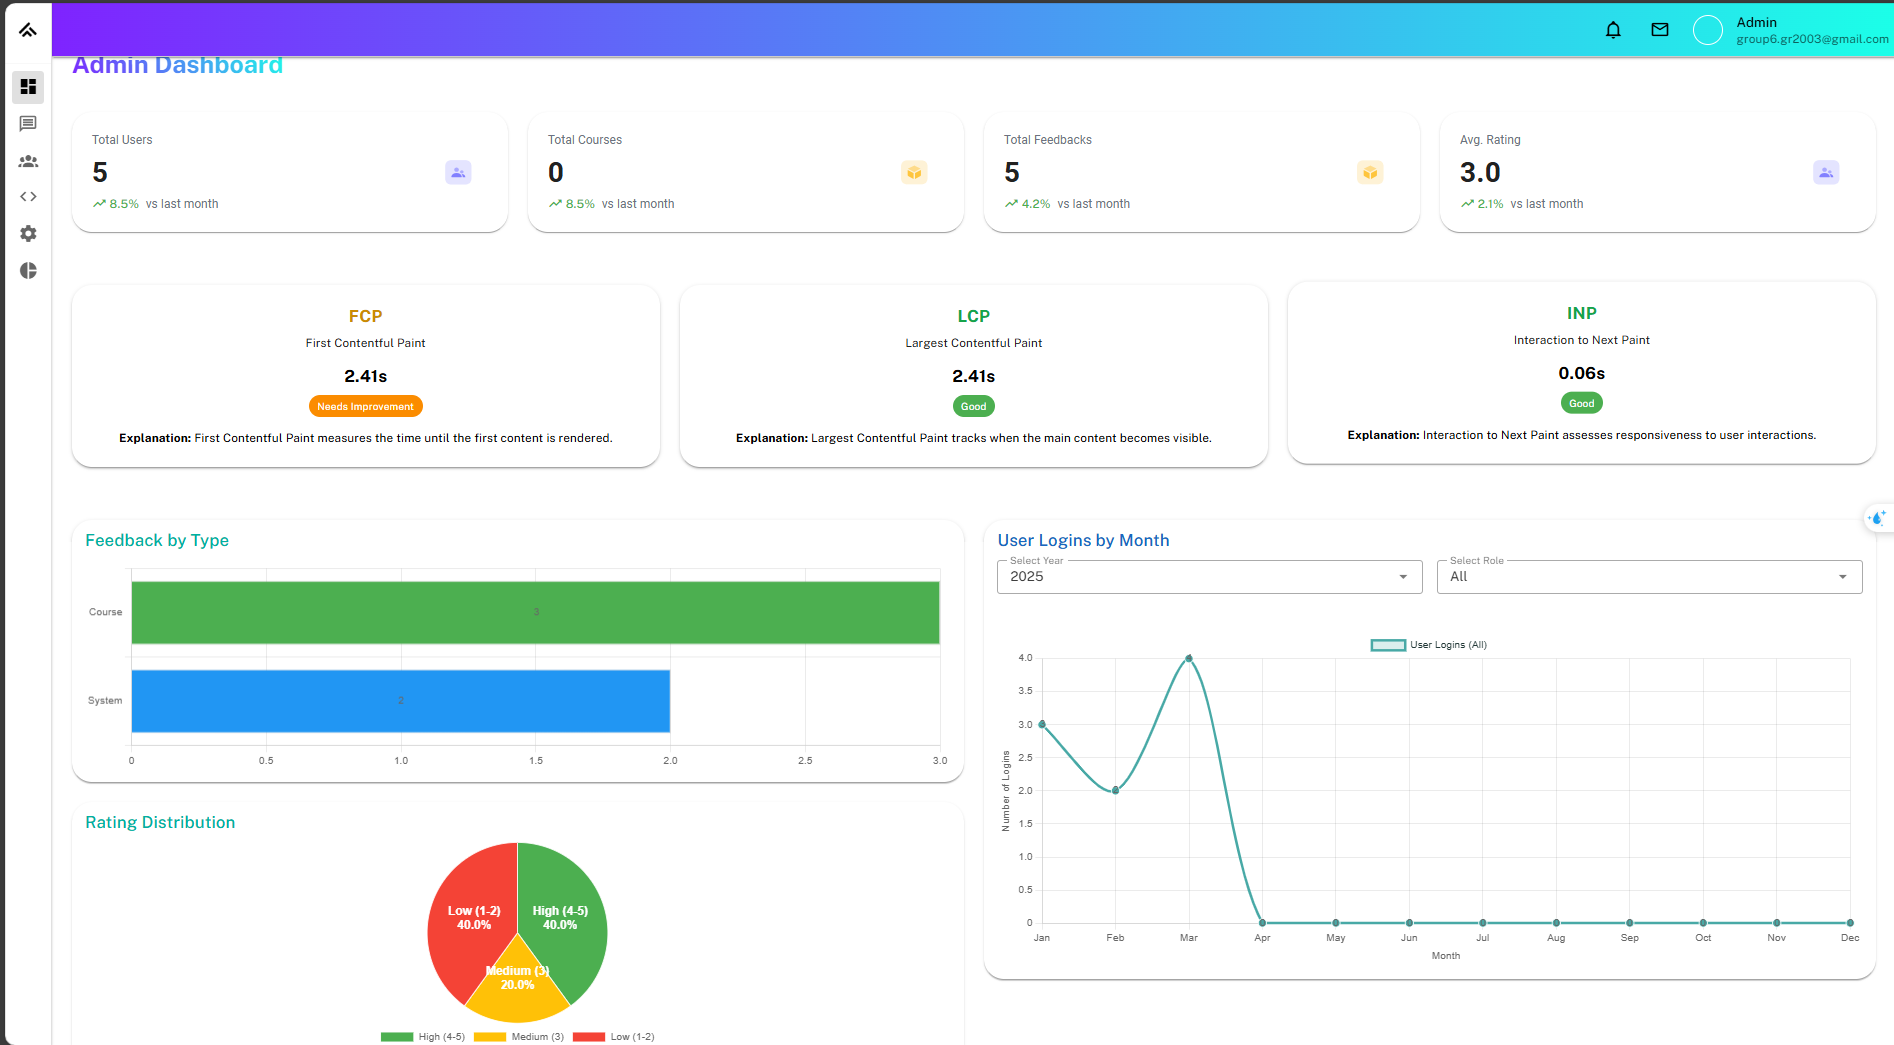
\includegraphics[width=0.8\linewidth]{images/admin_dashboard.png}
    \caption{Dashboard Admin}
    \label{fig:enter-label}
\end{figure}
Dashboard Admin, trang này như bảng điều khiển trung tâm để quản trị viên giám sát hệ thống. Nó hiển thị nổi bật các số liệu thống kê chính như:

\begin{itemize}
    \item Tổng số phản hồi gửi bởi người dùng.
    \item Tổng số người dùng đã đăng ký (bao gồm sinh viên, giáo viên và quản trị viên).
    \item Tổng số khóa học được cung cấp.
\end{itemize}

Các số liệu này cung cấp một cái nhìn tổng quan về hoạt động và mức độ tương tác của hệ thống. Dashboard tích hợp thêm biểu đồ để minh họa xu hướng theo thời gian, chẳng hạn như feedback hàng tuần hoặc sự tăng trưởng người dùng. 
\subsection{Quản lí các khóa học}
\begin{figure}[H]
    \centering
    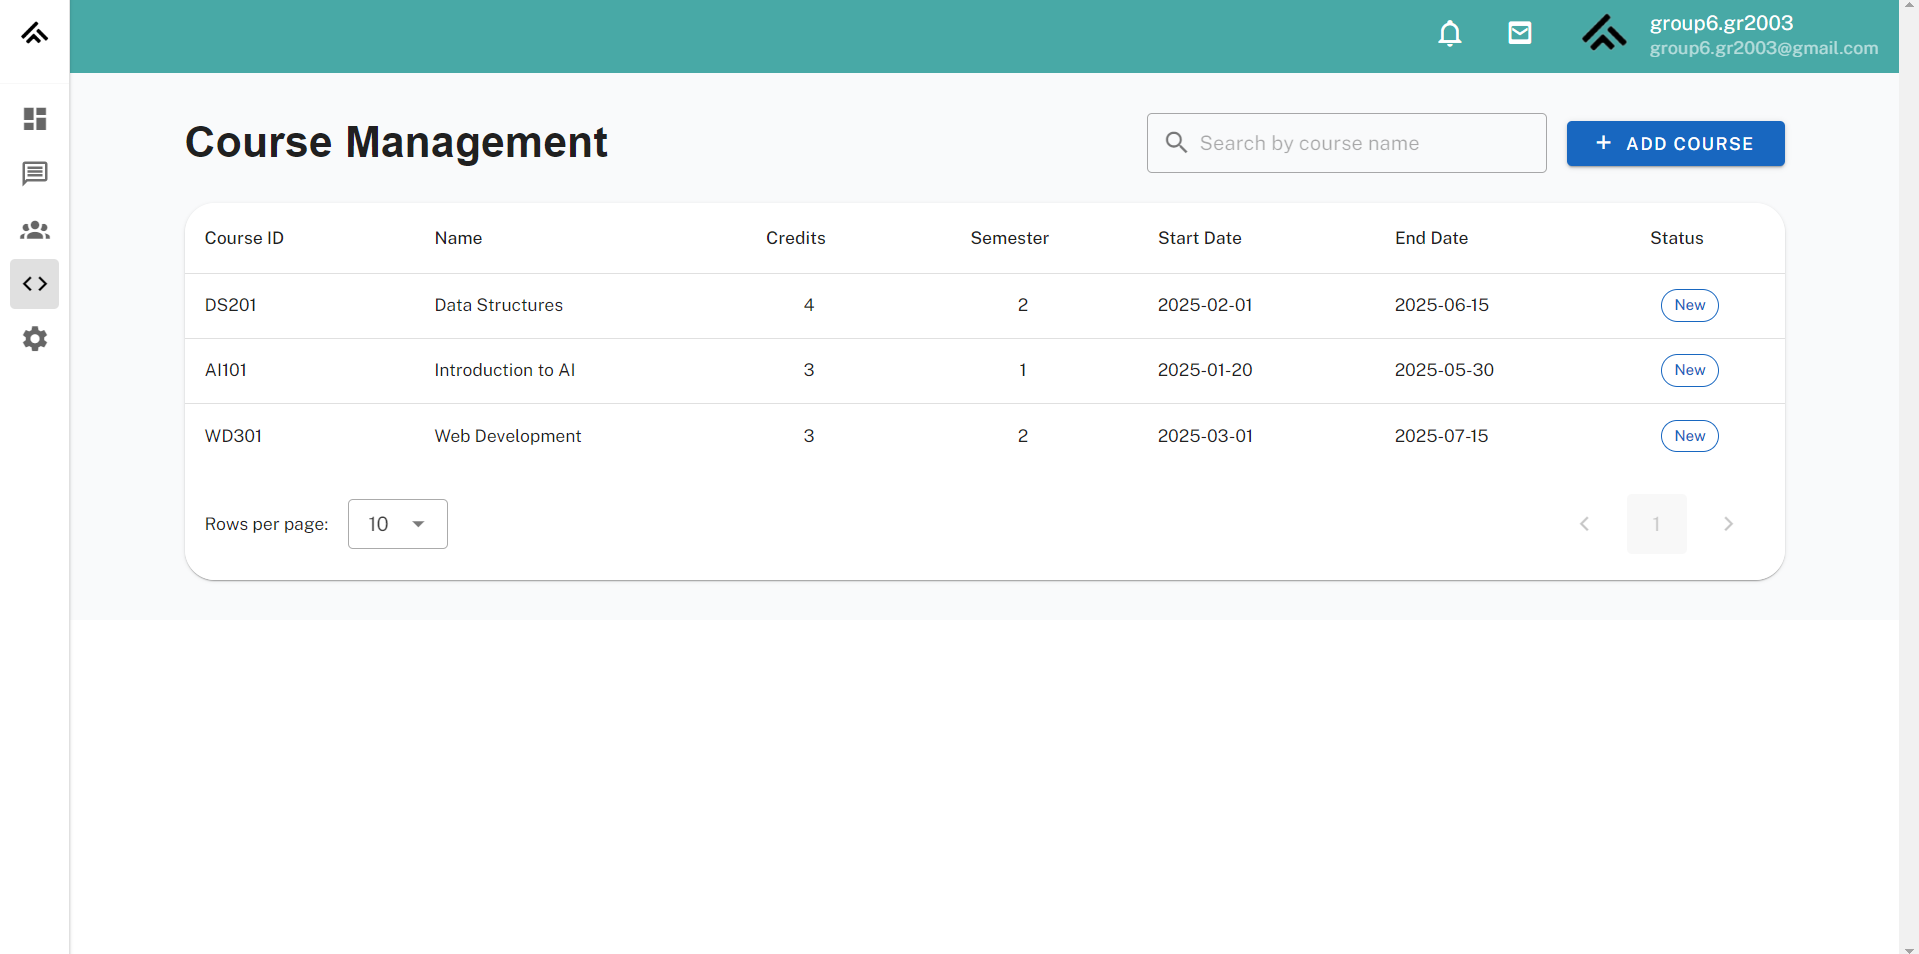
\includegraphics[width=0.8\linewidth]{images/admin_course_management.png}
    \caption{Quản lí danh sách khóa học của hệ thống}
    \label{fig:enter-label}
\end{figure}
Giao diện cung cấp một danh sách các khóa học với các cột chi tiết như:
\begin{itemize}
    \item Tiêu đề khóa học.
    \item Giáo viên, sinh viên được chỉ định.
    \item Số tín chỉ, học kì.
\end{itemize}

Quản trị viên có thể:
\begin{itemize}
    \item Chỉnh sửa chi tiết khóa học.
    \item Thêm khóa học mới.
    \item Xóa các khóa học.
\end{itemize}

\subsection{Thêm khóa học}
\begin{figure}[H]
    \centering
    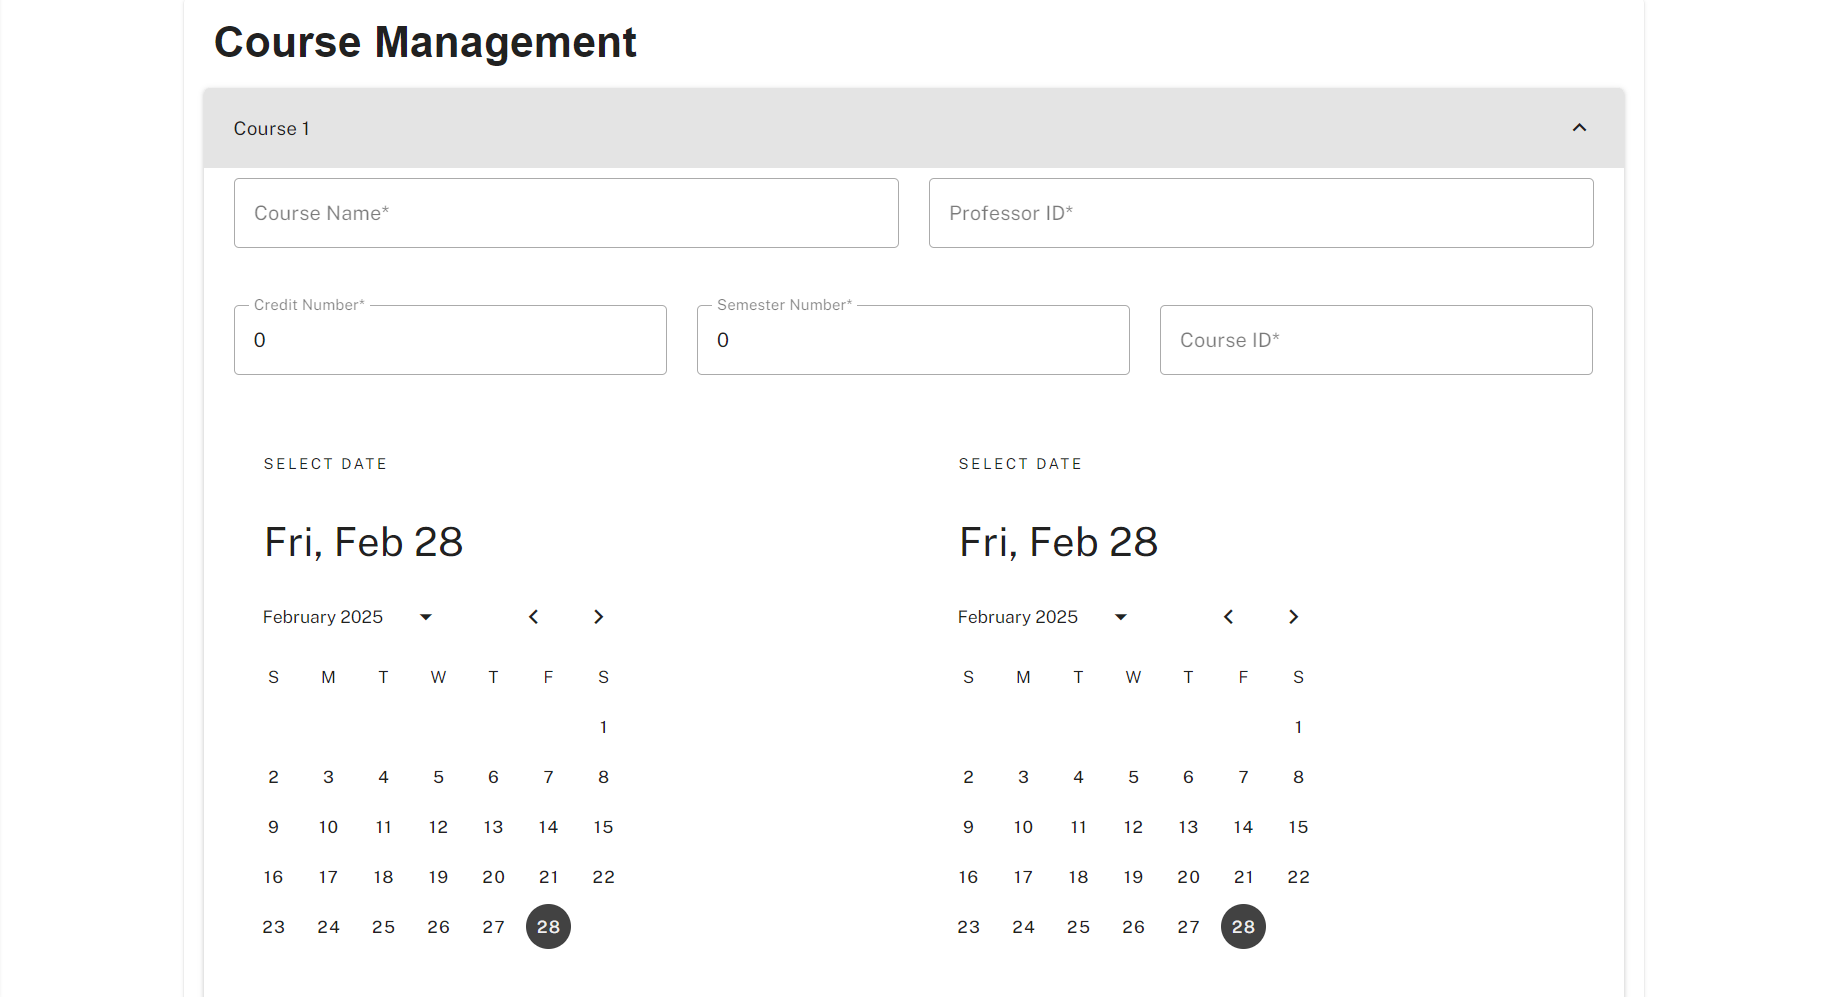
\includegraphics[width=0.8\linewidth]{images/admin_add_detail_course.png}
    \caption{Thông tin chi tiết khi thêm một khóa học}
    \label{fig:enter-label}
\end{figure}
Modal thêm khóa học bao gồm;
\begin{itemize}
    \item Tên khóa học: Mã định danh duy nhất.
    \item Mô tả khóa học: Tóm tắt mục tiêu và nội dung.
    \item Chỉ định giáo viên: ID của giáo viên phụ trách.
    \item Số tín chỉ, số học kì, thời gian khóa học
    \item Danh sách sinh viên
\end{itemize}
\begin{figure}[H]
    \centering
    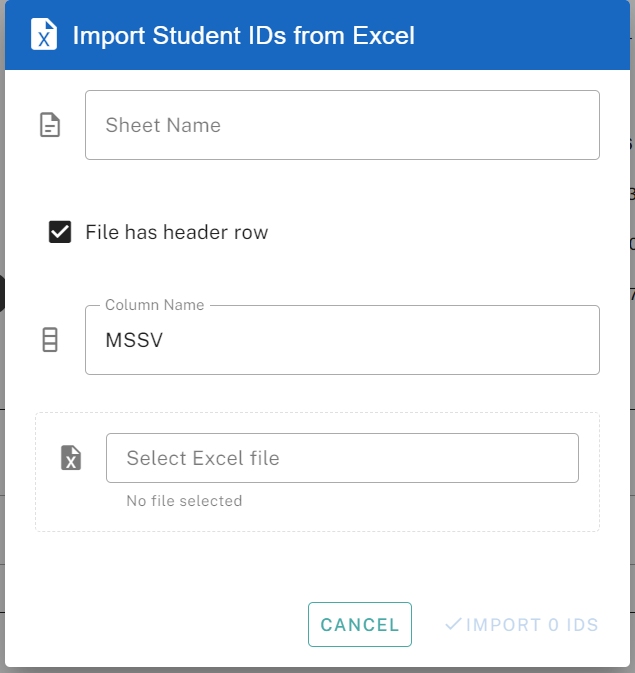
\includegraphics[width=0.6\linewidth]{images/admin_import_student_in_course.png}
    \caption{Thêm danh sách sinh viên vào khóa học}
    \label{fig:enter-label}
\end{figure}
Quá trình ghi danh sinh viên vào khóa học bằng cách nhập mã số từ tệp Excel. Tính năng này tối ưu hóa hiệu quả, đặc biệt với nhóm lớn. Giao diện cho phép:
\begin{itemize}
    \item Tải lên bảng Excel chứa mã số sinh viên (MSSV), tên, và có thể thêm email.
    \item Xác nhận tên sheet hoặc hàng tiêu đề để trích xuất dữ liệu chính xác.
\end{itemize}
So với nhập thủ công, quá trình này tiết kiệm thời gian và công sức, lý tưởng cho ghi danh hàng loạt vào đầu học kỳ hoặc chương trình đào tạo.
\begin{figure}[H]
    \centering
    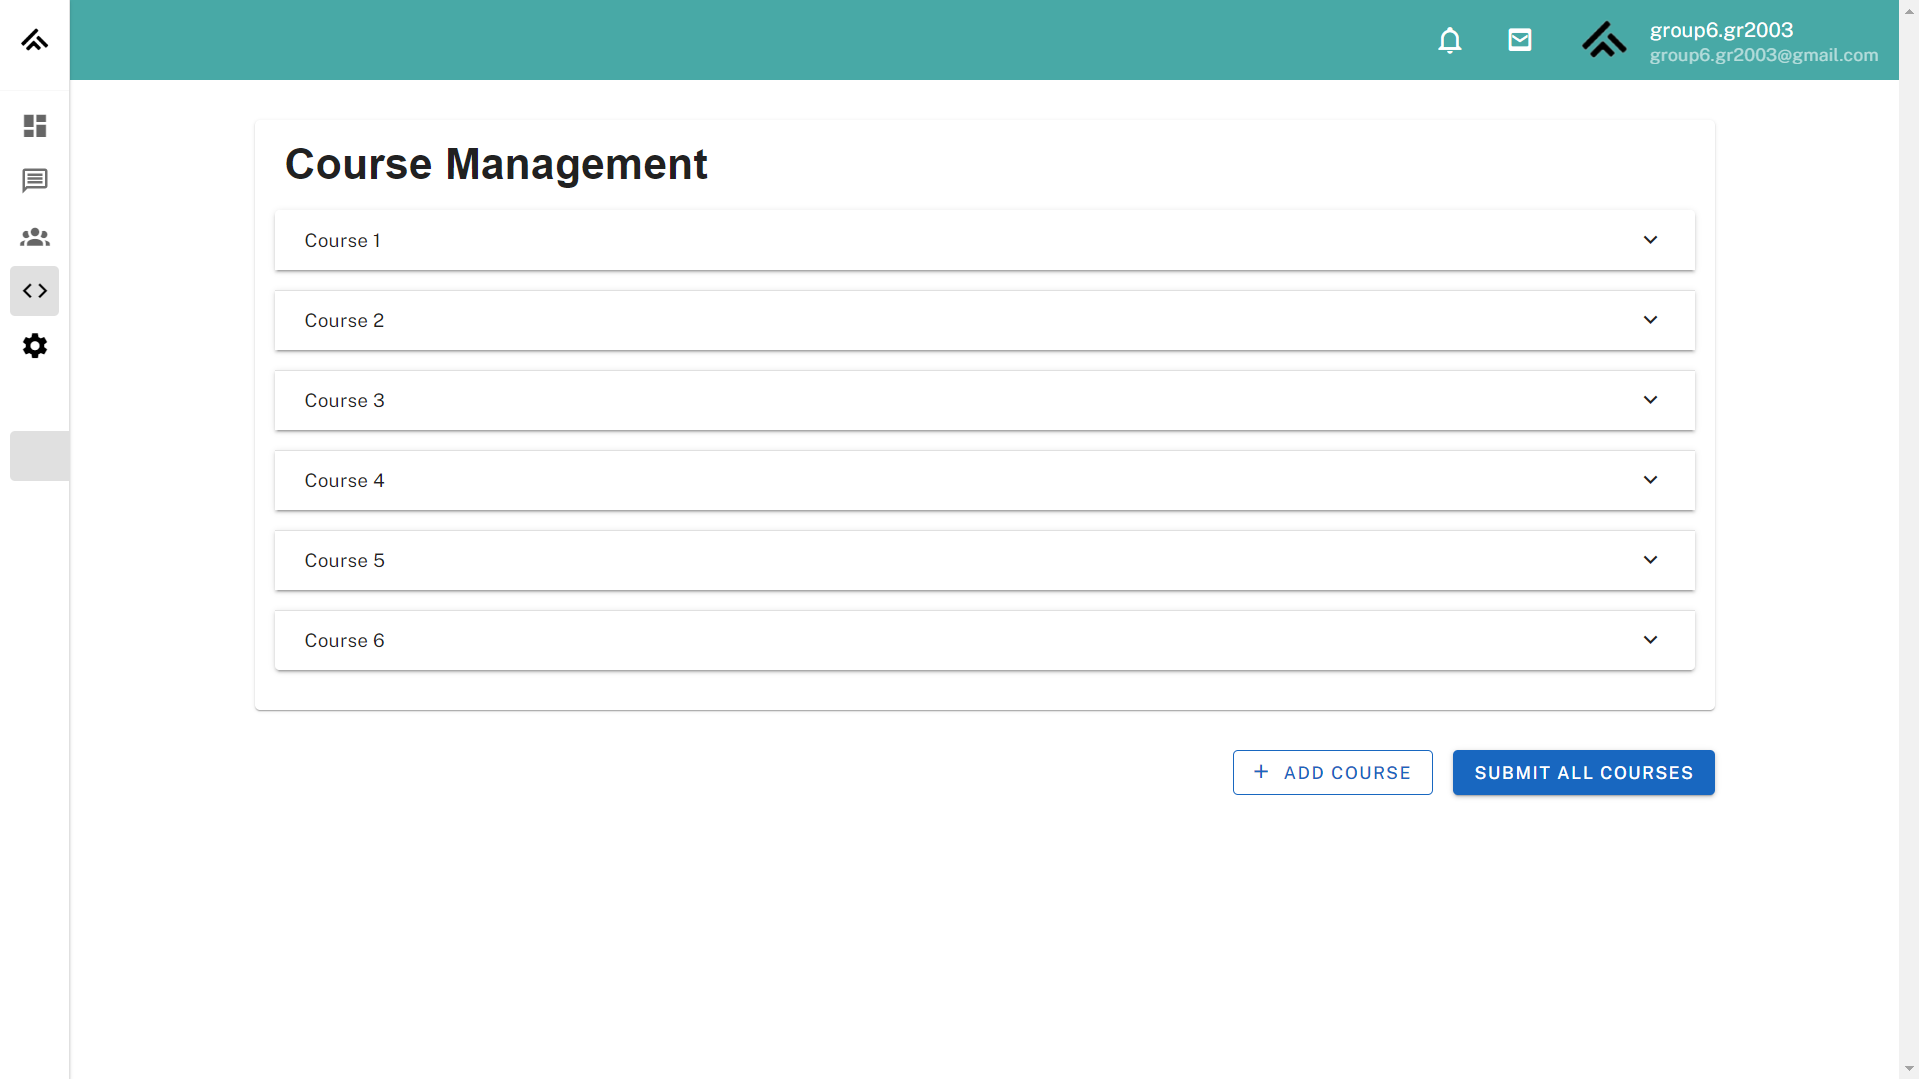
\includegraphics[width=0.6\linewidth]{images/admin_add_courses.png}
    \caption{Thêm nhiều khóa học}
    \label{fig:enter-label}
\end{figure}

Admin có thể thêm nhiều khóa học cùng một lúc.
\subsection{Thêm người dùng}
\begin{figure}[H]
    \centering
    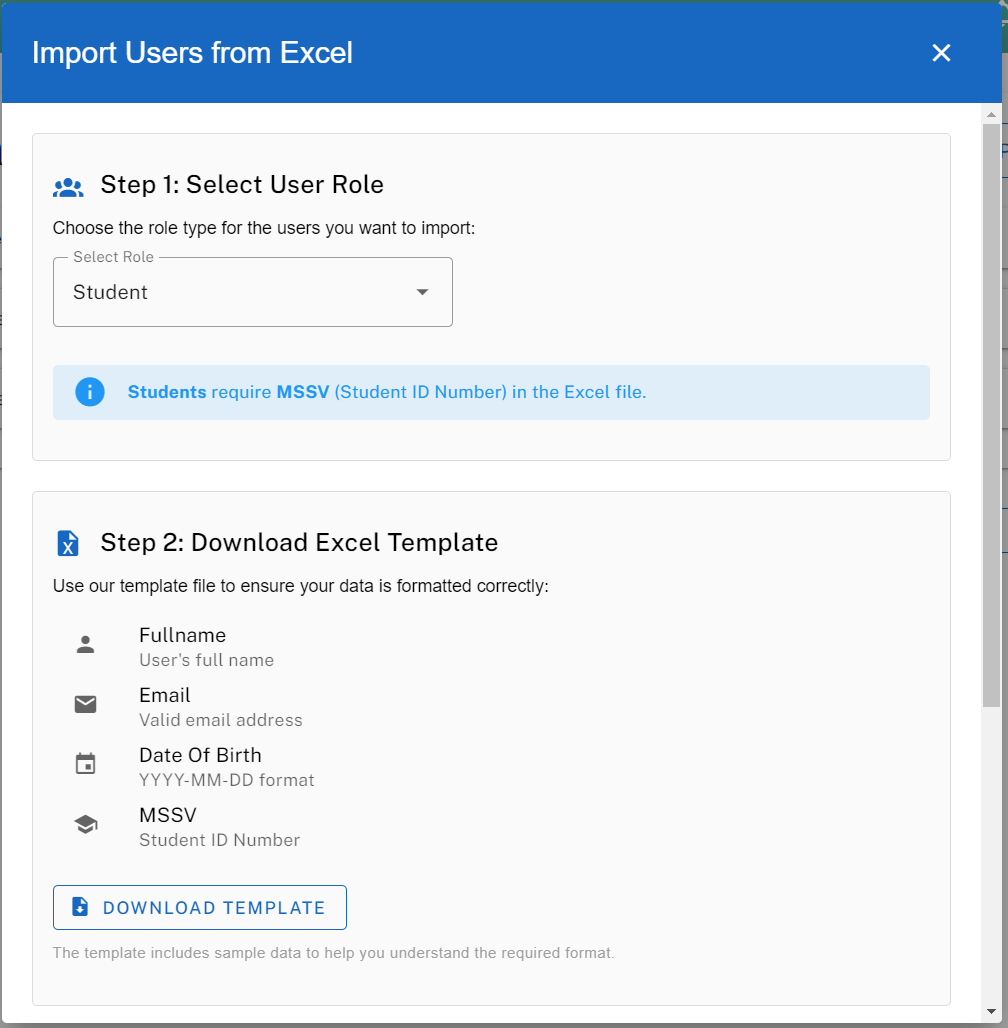
\includegraphics[width=0.6\linewidth]{images/admin_add_user_1.png}
    \caption{Thêm người dùng vào hệ thống }
    \label{fig:enter-label}
\end{figure}
\begin{figure}[H]
    \centering
    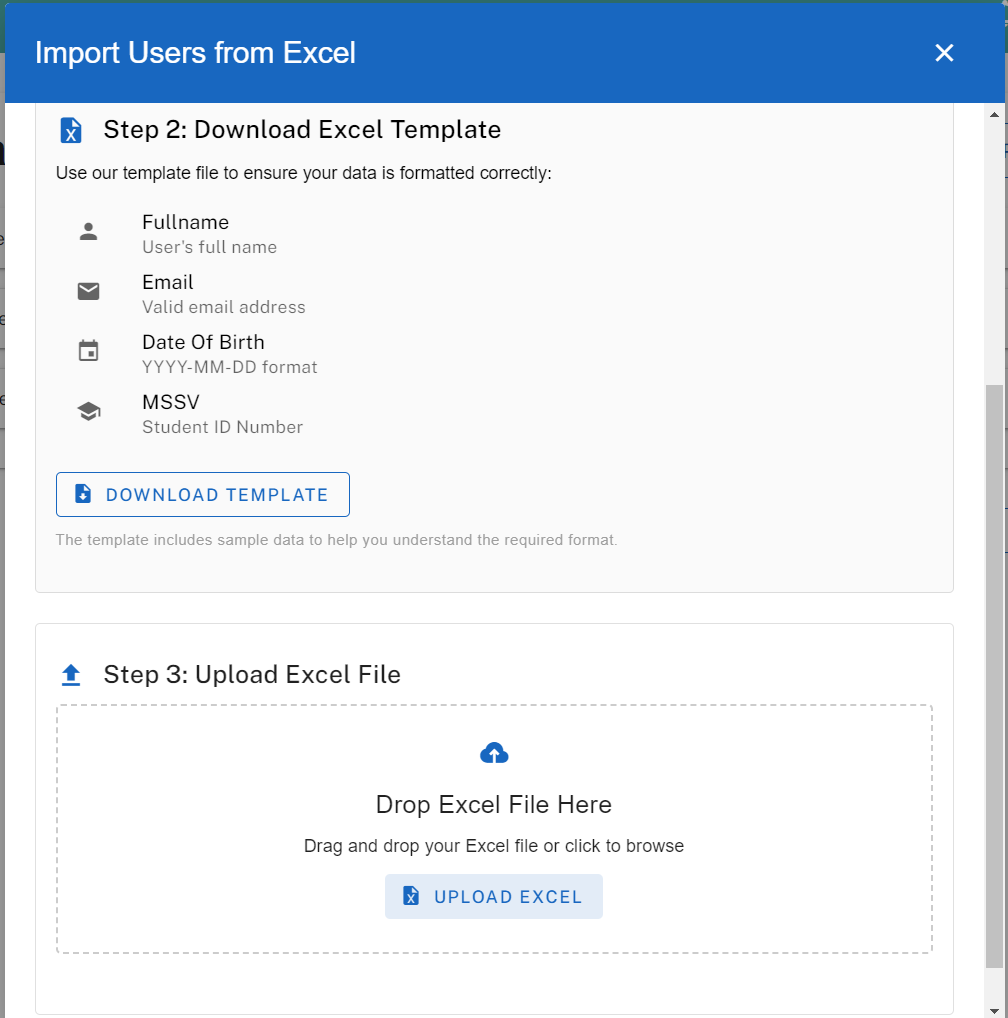
\includegraphics[width=0.6\linewidth]{images/admin_add_user_2.png}
    \caption{Caption}
    \label{fig:enter-label}
\end{figure}
Giao diện thêm người dùng mới (sinh viên, giáo viên, hoặc quản trị viên) vào nền tảng. Quản trị viên có thể:
\begin{itemize}
    \item Nhập dữ liệu từ mẫu Excel với thông tin như tên, mã số (MSSV), email, và vai trò.
    \item Cài đặt quyền theo vai trò (ví dụ: giáo viên tạo khóa học, sinh viên chỉ học).
\end{itemize}
\section{Code Area}
\subsection{Sử dụng Judge0 API}
\begin{itemize}
    \item Judge0 API là một hệ thống thực thi mã nguồn trực tuyến mã nguồn mở tiên tiến, được thiết kế để mạnh mẽ và có khả năng mở rộng. Đây là một công cụ cho phép thực hiện việc chạy mã nguồn trong nhiều ngôn ngữ lập trình khác nhau
    \item Điểm nổi bật của Judge0 là tính linh hoạt và khả năng tùy chỉnh. Judge0 API cho phép tùy chọn biên dịch, thêm đối số dòng lệnh, hoặc đặt giới hạn về thời gian và bộ nhớ khi thực thi mã nguồn. Điều này đặc biệt quan trọng nếu bạn dùng Judge0 trong các tác vụ đòi hỏi hiệu suất cao.
    \item Judge0 API hỗ trợ hơn 60 ngôn ngữ lập trình, từ những ngôn ngữ phổ biến mà bạn có thể đã sử dụng đến những ngôn ngữ ít gặp hơn.
\end{itemize}


\subsection{Thiết kế chức năng cho student làm bài tập: code}
\begin{figure}[H]
    \centering
    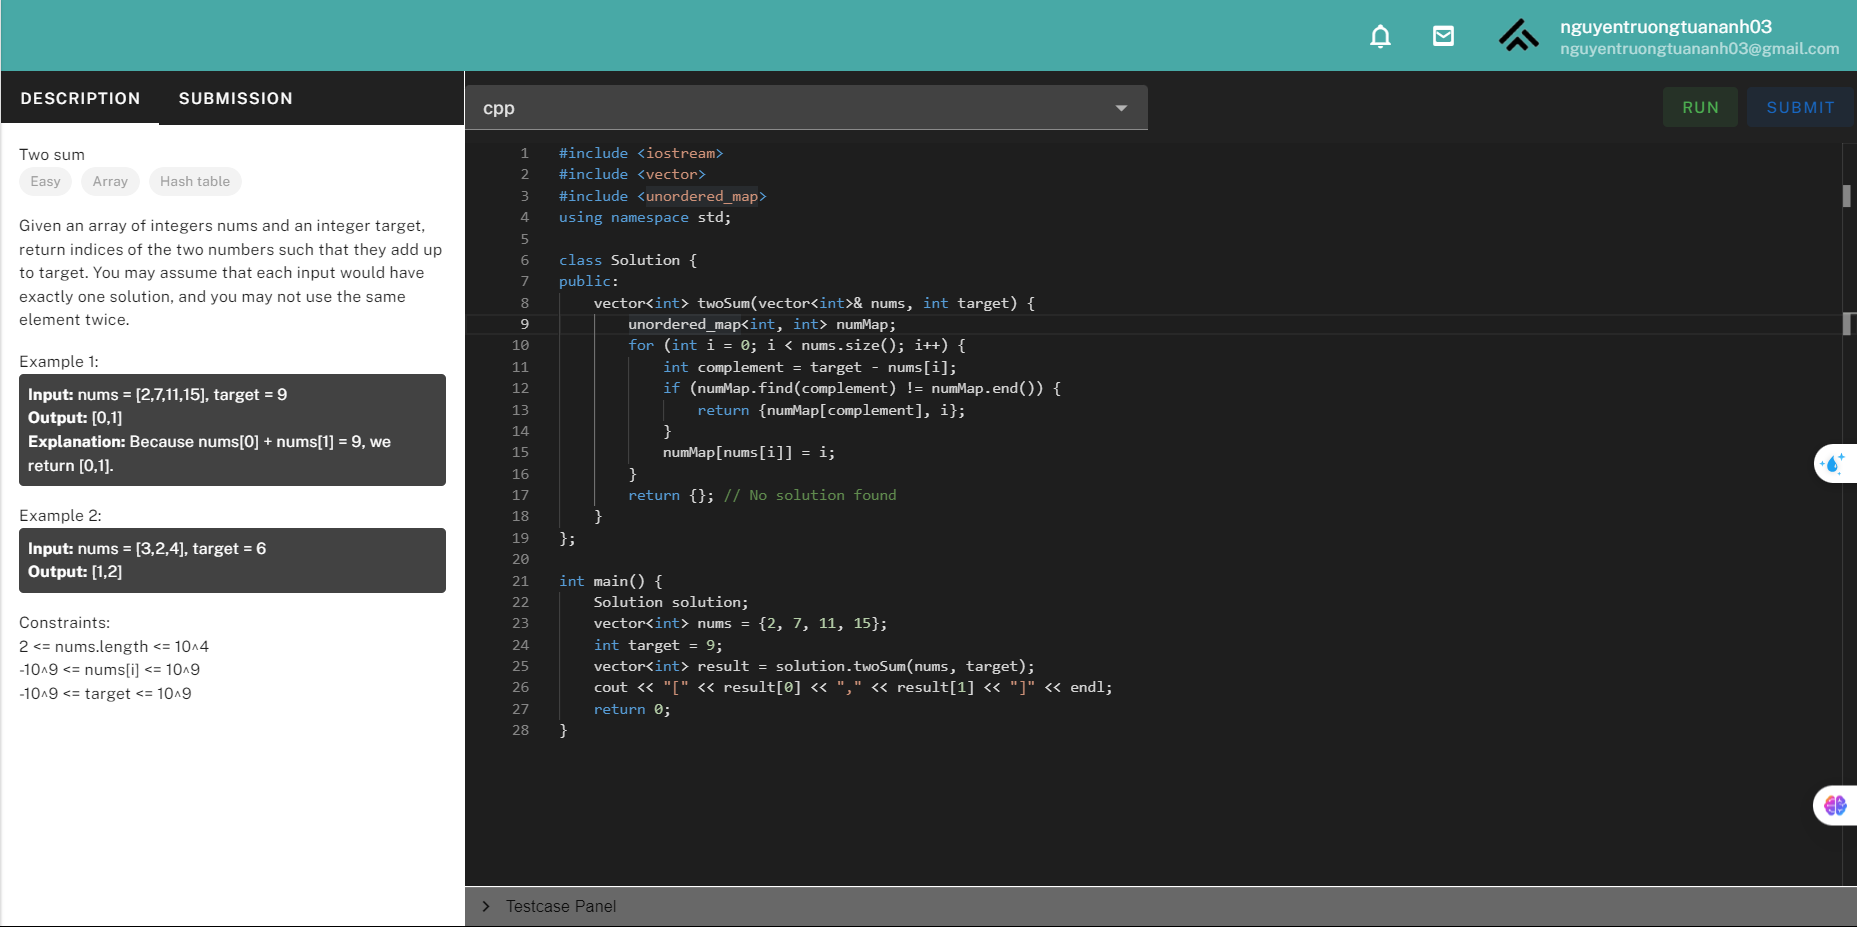
\includegraphics[width=0.8\linewidth]{images/code_area.png}
    \caption{Khu vực làm bài tập code}
    \label{fig:enter-label}
\end{figure}
Sinh viên có thể chọn ngôn ngữ lập trình, xem hướng dẫn, và truy cập mẫu đầu vào/đầu ra. Thiết lập này mô phỏng công cụ phát triển chuyên nghiệp, kết nối lý thuyết và thực hành. Tích hợp API Judge0 cung cấp đánh giá mã tự động, mang lại phản hồi tức thì để cải thiện kỹ năng học tập.
\begin{figure}[H]
    \centering
    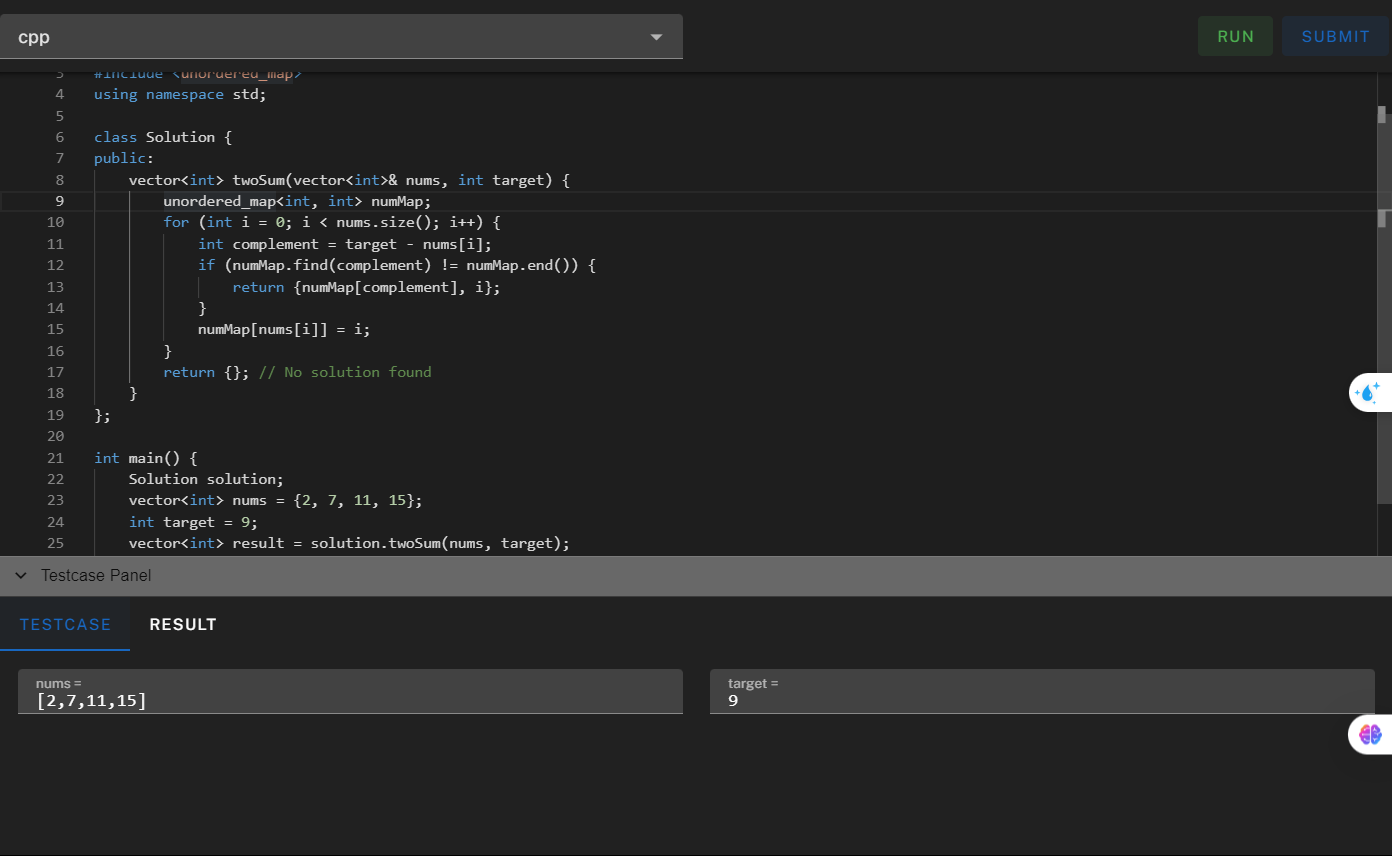
\includegraphics[width=0.8\linewidth]{images/code_testcase.png}
    \caption{Testcase bài tập}
    \label{fig:enter-label}
\end{figure}
Gaio diện hiển thị các testcase cho bài tập lập trình, cần thiết để đánh giá bài code của sinh viên. Mỗi trường hợp bao gồm:
\begin{itemize}
    \item Đầu vào cụ thể và đầu ra dự kiến.
    \item Một số hiển thị để hướng dẫn, một số ẩn để kiểm tra toàn diện.
\end{itemize}

\begin{figure}[H]
    \centering
    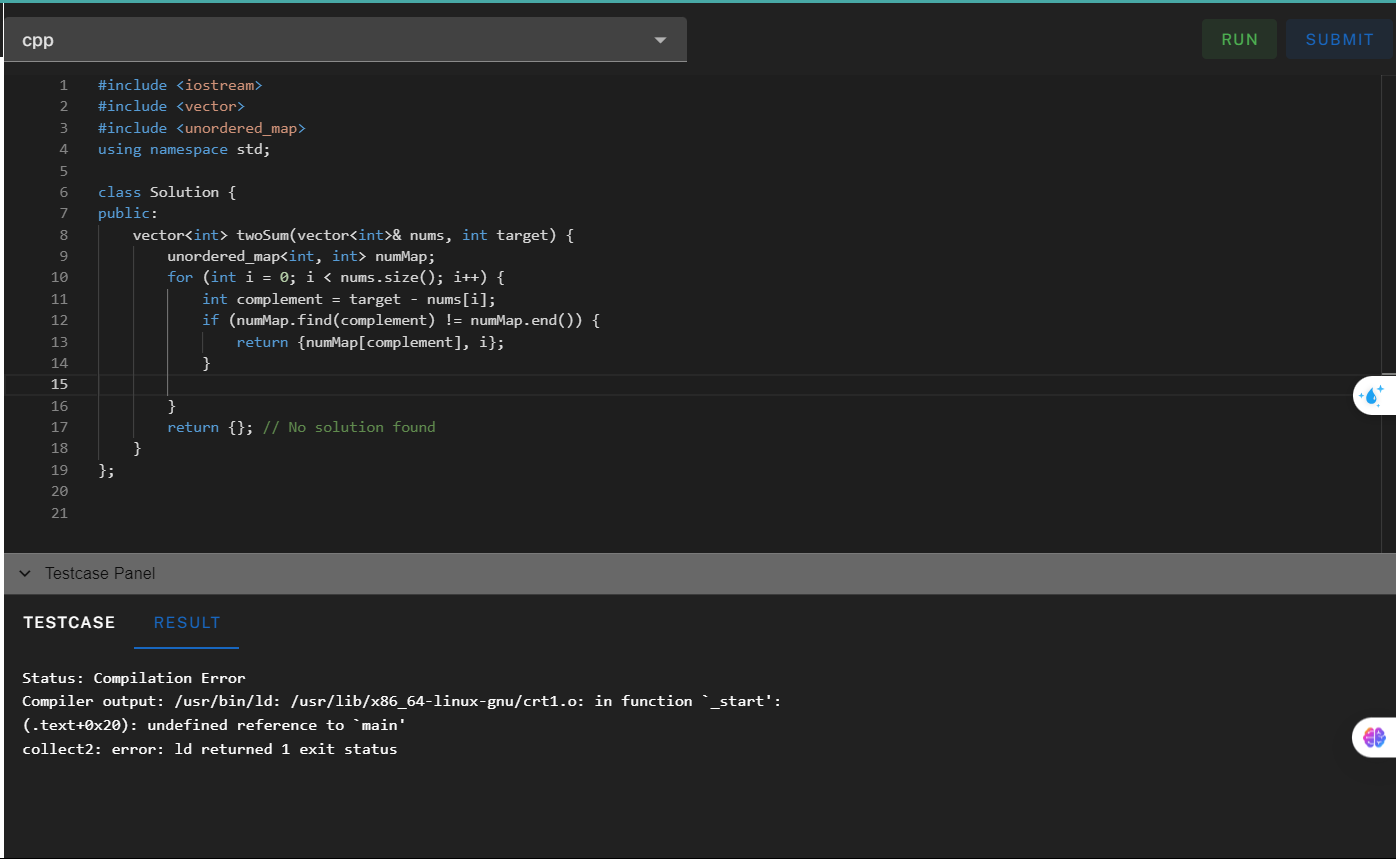
\includegraphics[width=0.8\linewidth]{images/code_run_error.png}
    \caption{Thông báo kết quả khi code chạy lỗi}
    \label{fig:enter-label}
\end{figure}
Kết quả thông báo lỗi khi đoạn code sinh viên lỗi
\begin{itemize}
    \item Loại lỗi: Cú pháp, thời gian chạy, v.v.
    \item Số dòng: Vị trí lỗi.
    \item Phản hồi chi tiết giúp sinh viên xác định sai lầm, hiểu nguyên nhân, và học hỏi.
\end{itemize}
\begin{figure}[H]
    \centering
    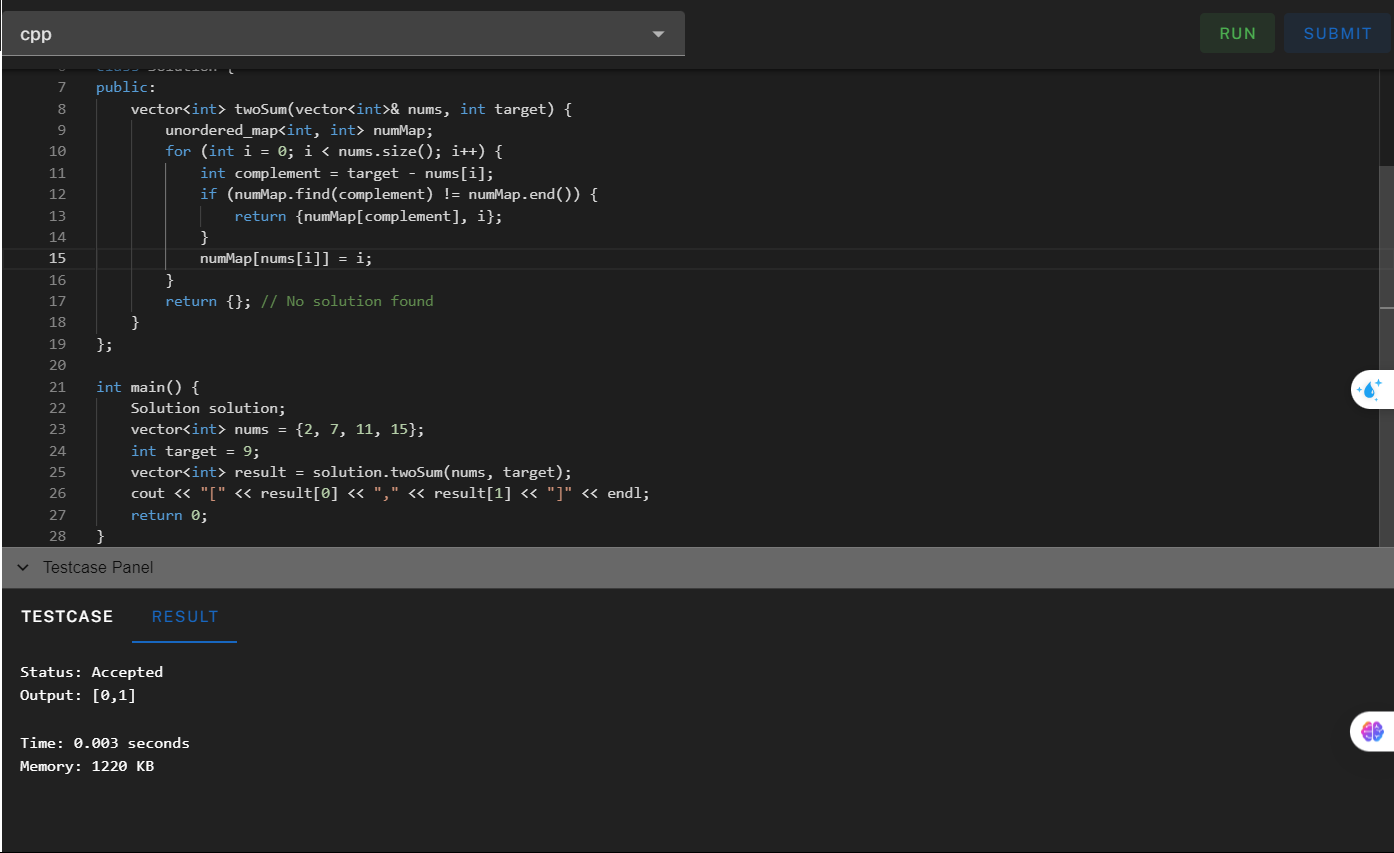
\includegraphics[width=0.8\linewidth]{images/code_run_success.png}
    \caption{Thông báo kết quả khi code chạy thành công}
    \label{fig:enter-label}
\end{figure}
Kết quả thông báo khi đoạn code sinh viên chạy thành công
\begin{itemize}
    \item Số trường hợp kiểm thử đã qua.
    \item Chỉ số hiệu suất (thời gian thực thi, bộ nhớ).
    \item Thông báo này củng cố tích cực, cung cấp cái nhìn về hiệu quả mã.
\end{itemize}
% \section{Authentication}
\subsection{Tổng quan}
Hệ thống  được xây dựng với các tính năng bảo mật cao, hỗ trợ đa dạng phương thức xác thực bao gồm:
\begin{itemize}
    \item Xác thực email thông qua verification code
    \item Quản lý phiên đăng nhập với JWT (Access token \& Refresh token)
    \item Chức năng quên và đặt lại mật khẩu
\end{itemize}
\subsection{Chi tiết triển khai}
\subsubsection{Quản lí token:}
Hệ thống sử dụng cơ chế JWT với 2 loại token:
\begin{itemize}
    \item \textbf{Access token:}
    \begin{itemize}
        \item Thời gian sống ngắn (mặc định 15 phút)
        \item Sử dụng SECRET\_KEY riêng để mã hóa
        \item Chứa thông tin user ID trong claim "sub"
        \item Có thể tùy chỉnh thời gian hết hạn
    \end{itemize}
    \item \textbf{Refresh Token:}
    \begin{itemize}
        \item Thời gian sống dài (cấu hình theo số ngày): 7 ngày
        \item Sử dụng REFRESH\_SECRET\_KEY riêng biệt
        \item Dùng để cấp mới access token khi hết hạn
        \item Tích hợp xử lý lỗi khi token hết hạn hoặc không hợp lệ
    \end{itemize}
\end{itemize}
\subsubsection{Các API endpoint}
\textbf{Xác thực email và đăng ký:}
\begin{itemize}
    \item \textbf{/verify-email:} Xác thực email thông qua mã code
    \begin{figure}[H]
        \centering
        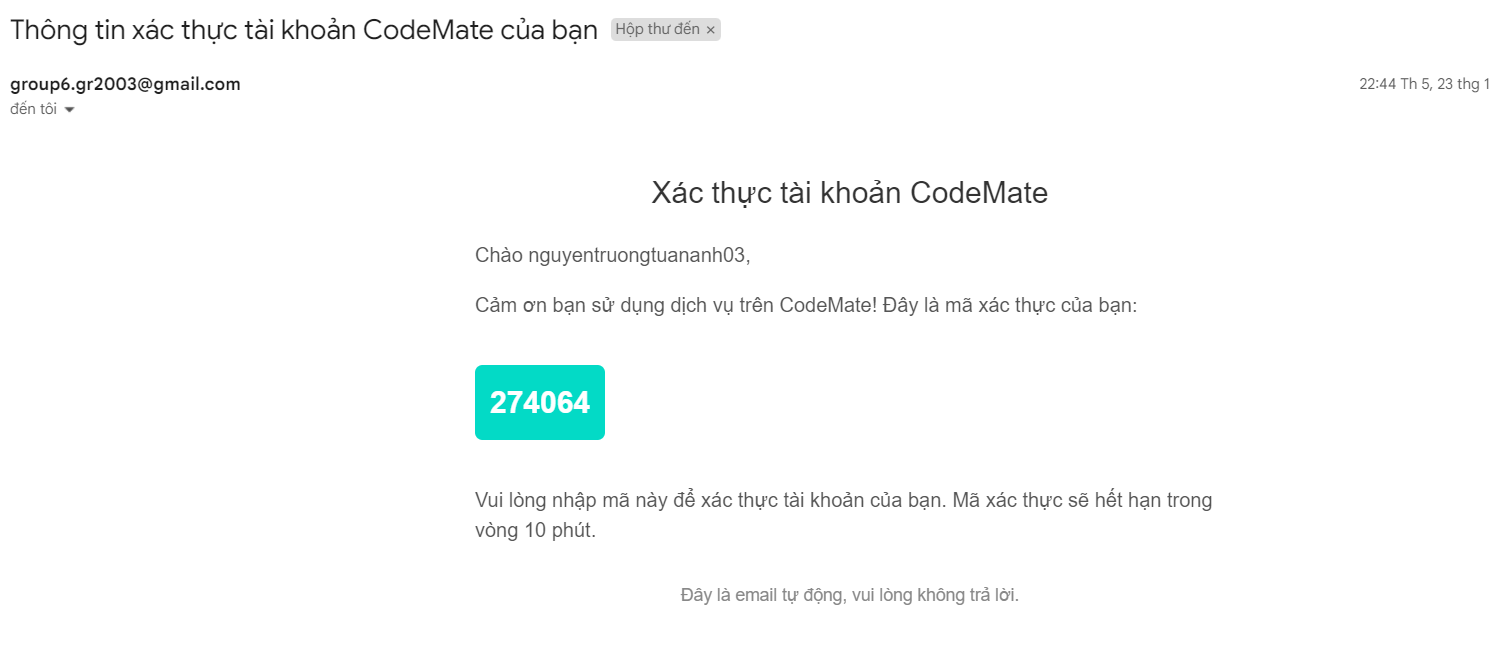
\includegraphics[width=0.8\linewidth]{images/verify_email.png}
        \caption{Xác thực email thông qua mã code}
        \label{fig:enter-label}
    \end{figure}
    \item \textbf{/resend-verification-code:} Gửi lại mã xác thực
\end{itemize}
\textbf{Quản lý Mật khẩu:}
\begin{itemize}
    \item \textbf{/forgot-password:} Khởi tạo quy trình quên mật khẩu
    \begin{figure}[H]
        \centering
        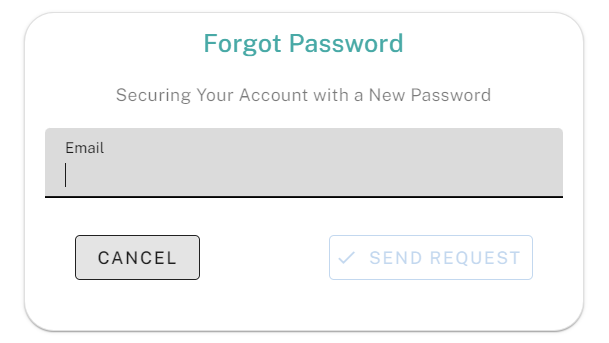
\includegraphics[width=0.6\linewidth]{images/forgot_password.png}
        \caption{Quên mật khẩu}
        \label{fig:enter-label}
    \end{figure}
    \item \textbf{/reset-password:} Đặt lại mật khẩu mới
    \item Sử dụng hash\_password để mã hóa mật khẩu an toàn
\end{itemize}

\section{Login}
\subsection{Tổng quan:}
Hệ thống có thể đăng nhập thông qua 2 phương thức:
\begin{itemize}
    \item Đăng nhập bằng email trường cấp (cho sinh viên và giảng viên)
    \item Đăng nhập với Google
\end{itemize}
\subsection{Chi tiết triển khai:}
\textbf{Trang giới thiệu:}
\begin{figure}[H]
        \centering
        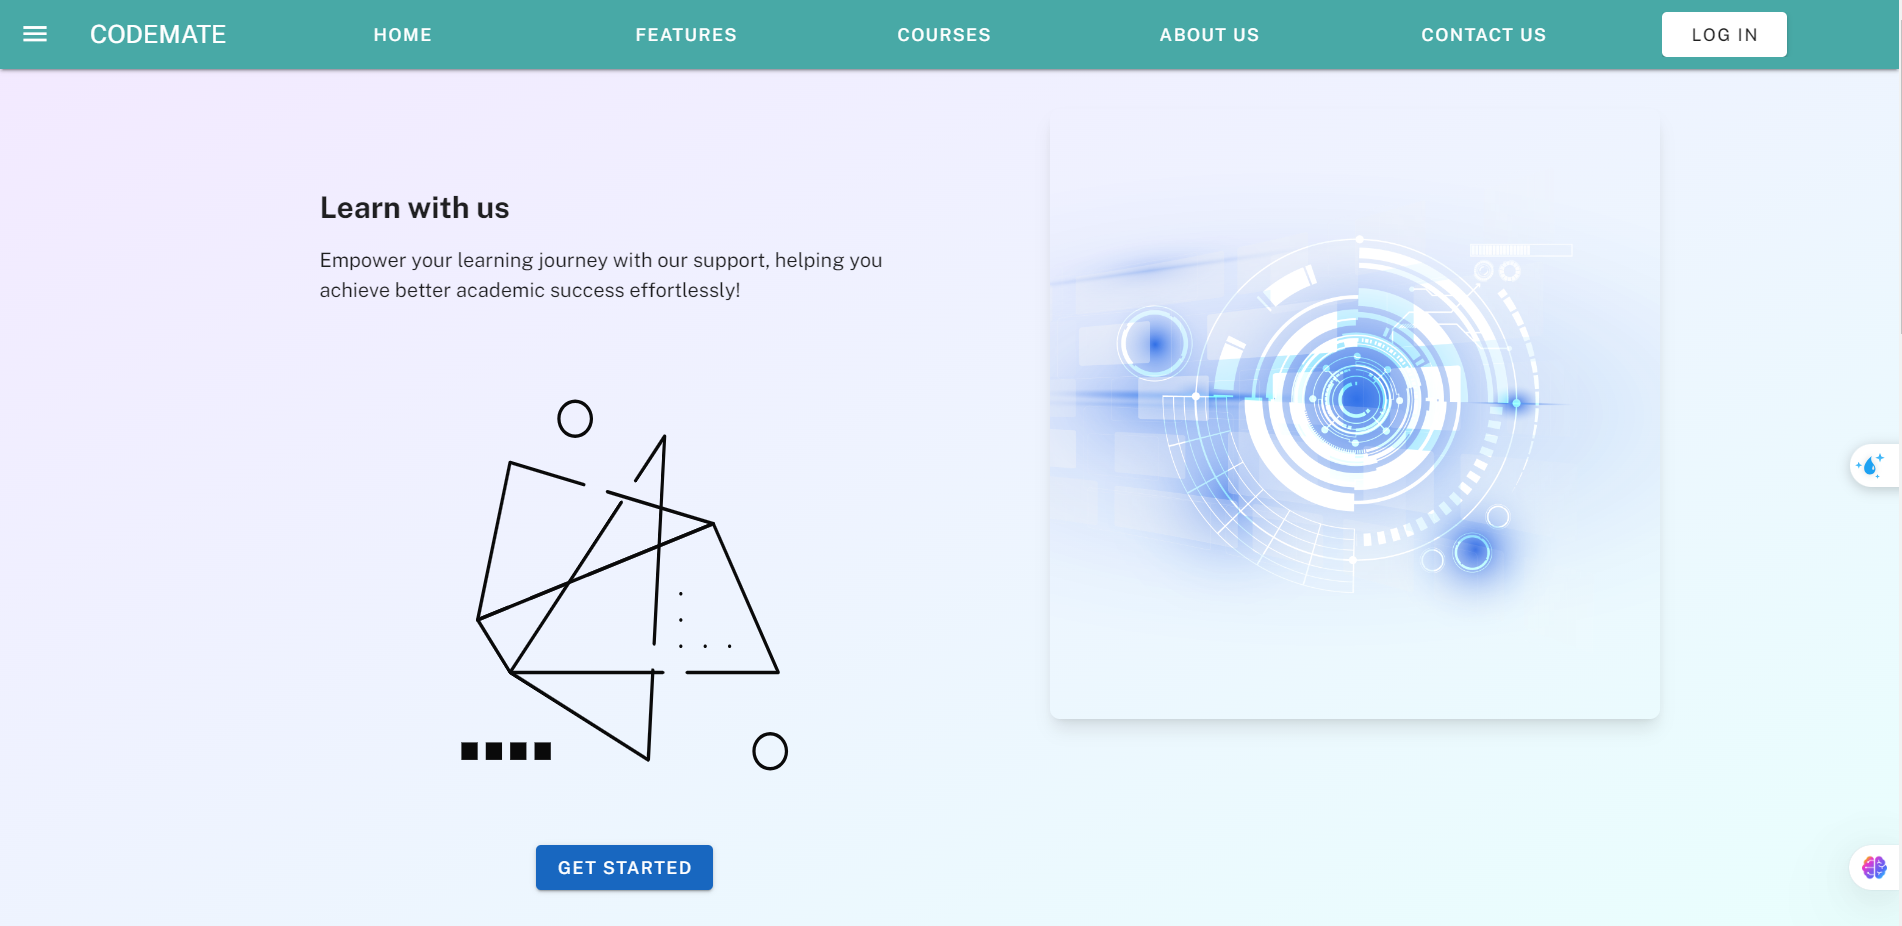
\includegraphics[width=0.8\linewidth]{images/introduction.png}
        \caption{Trang khởi đầu của hệ thống}
        \label{fig:enter-label}
    \end{figure}
\begin{figure}[H]
        \centering
        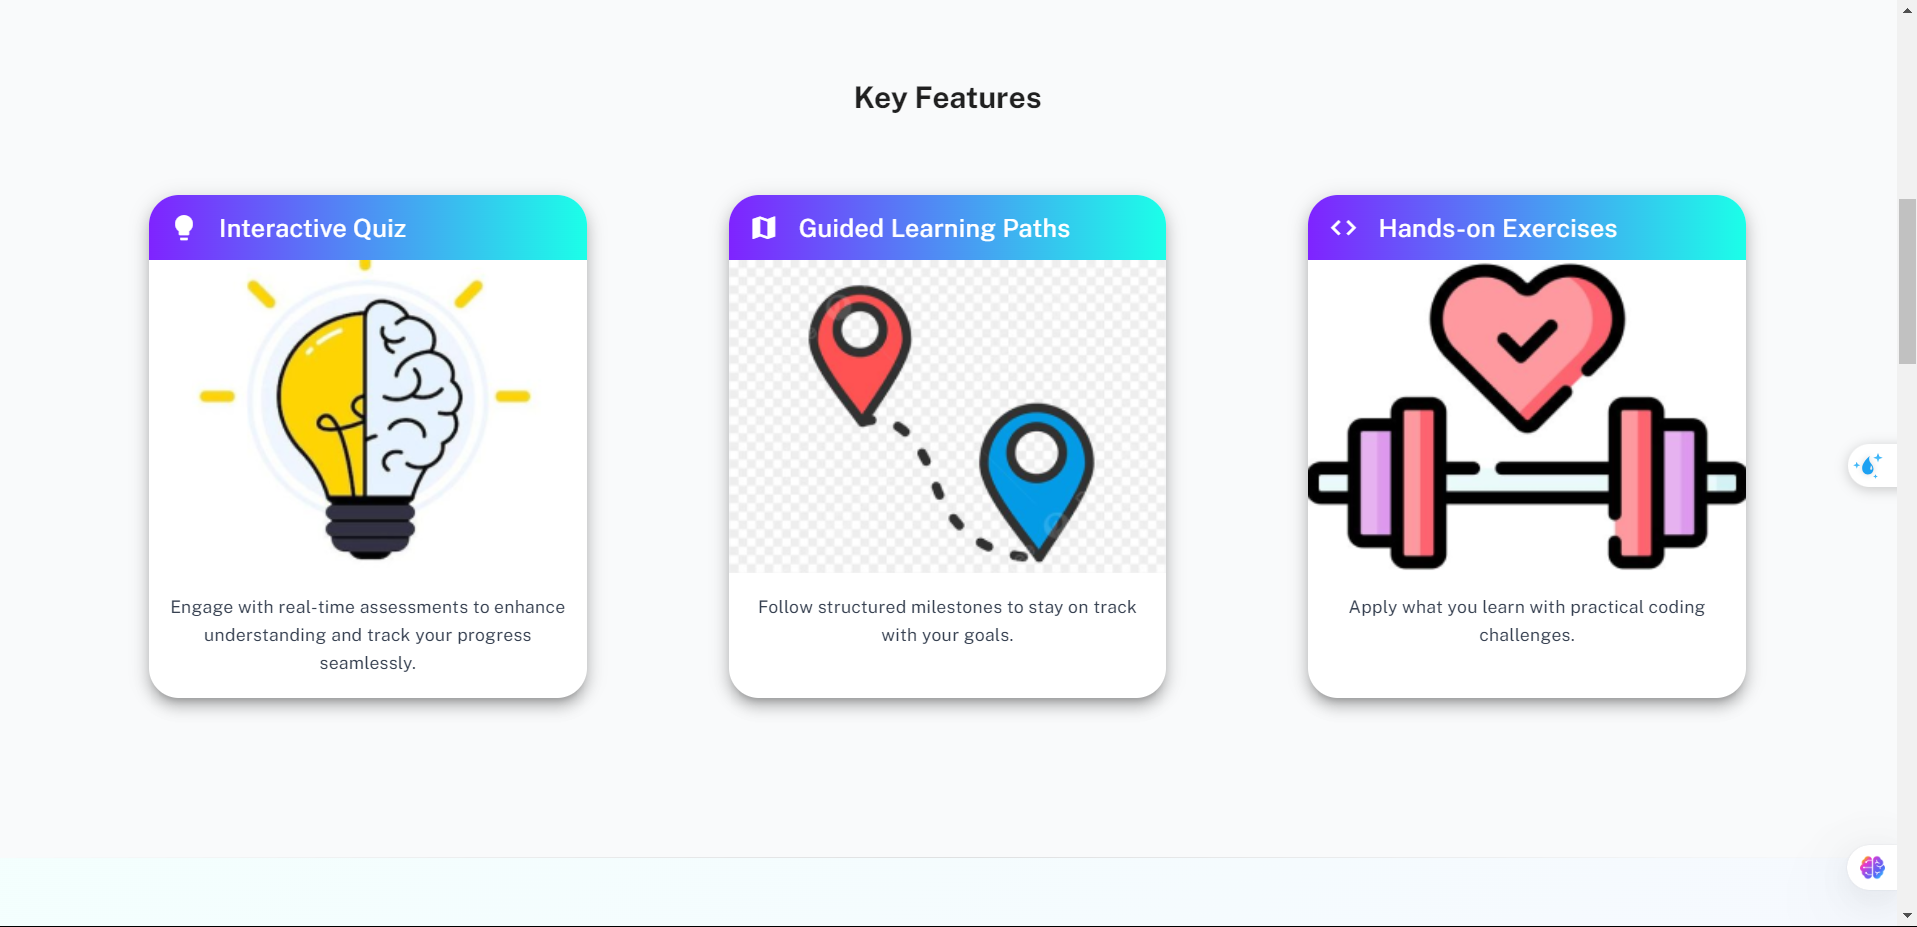
\includegraphics[width=0.8\linewidth]{images/introduction_feature.png}
        \caption{Giới thiệu các tính năng nổi bật}
        \label{fig:enter-label}
    \end{figure}
    \begin{figure}[H]
        \centering
        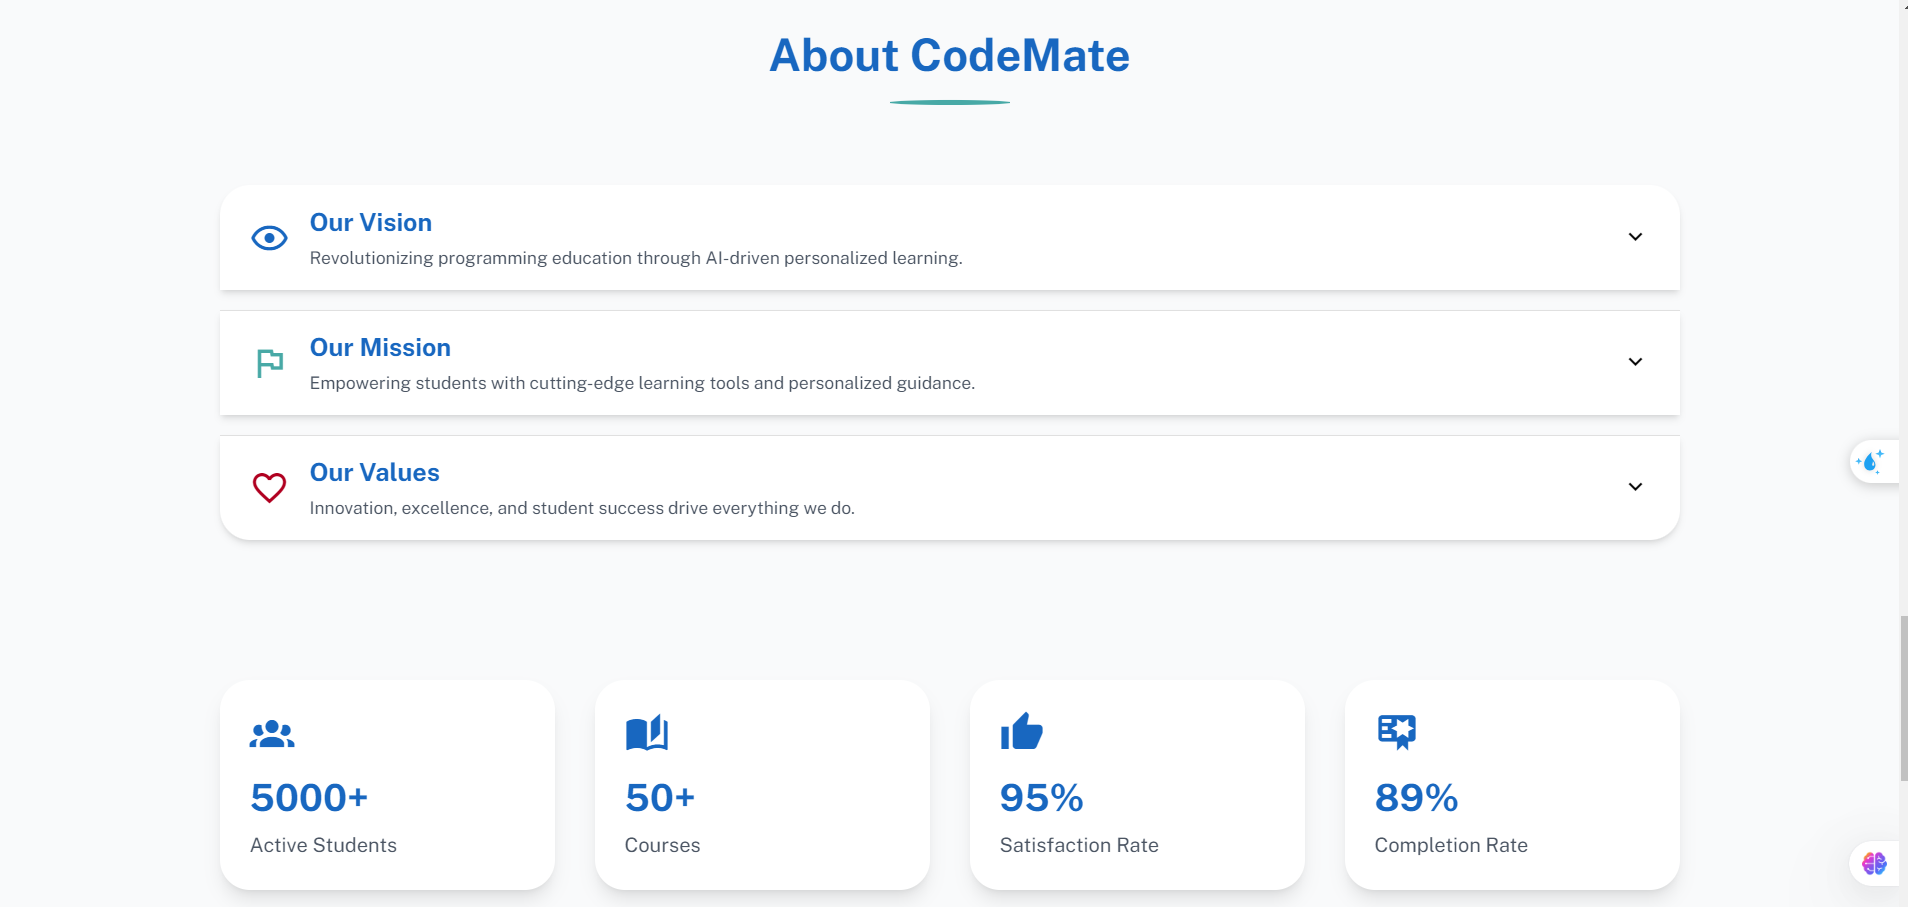
\includegraphics[width=0.8\linewidth]{images/introduction_about.png}
        \caption{Giới thiệu về hệ thống Codemate}
        \label{fig:enter-label}
    \end{figure}
    \begin{figure}[H]
        \centering
        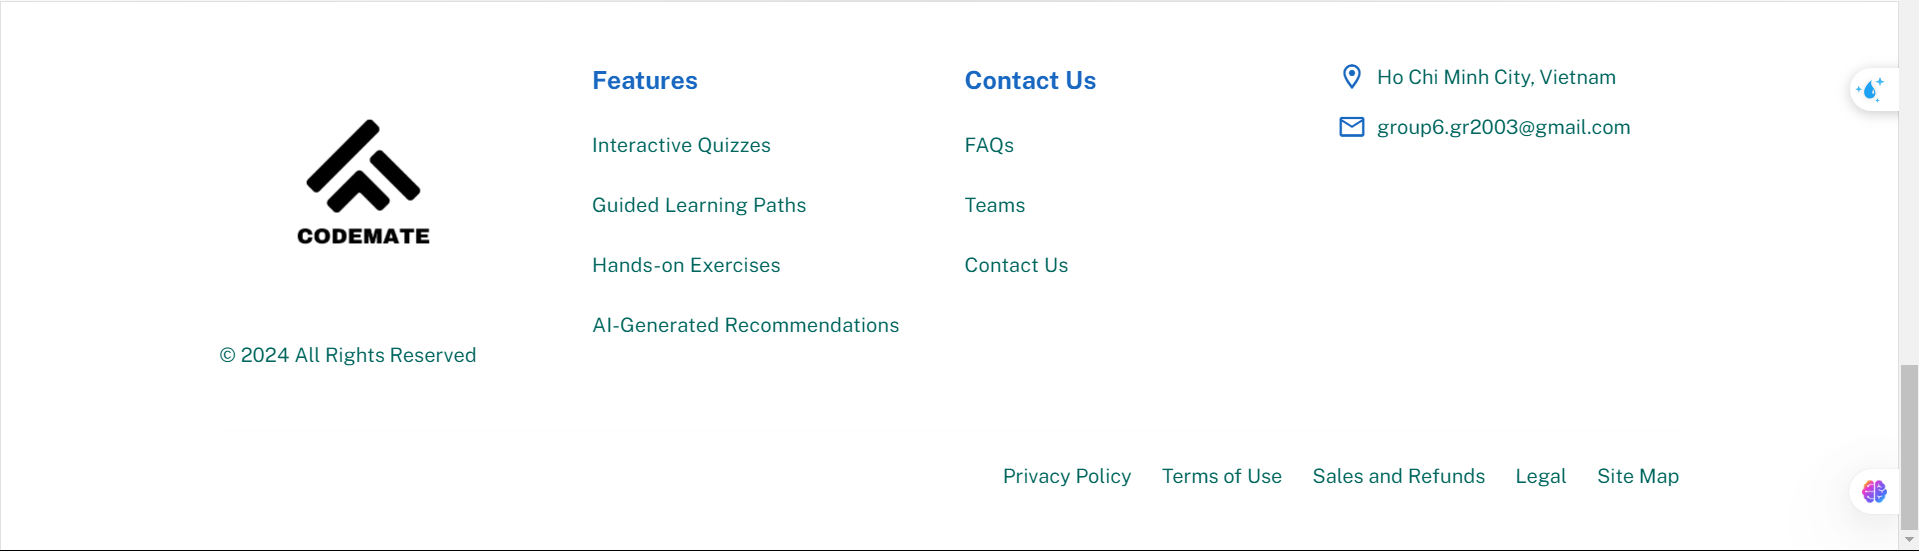
\includegraphics[width=0.8\linewidth]{images/introduction_contact.png}
        \caption{Thông tin liên hệ}
        \label{fig:enter-label}
    \end{figure}
\textbf{Đăng nhập bằng email trường:}
\begin{itemize}
    \item Kiểm tra thông tin đăng nhập: xác thực email và mật khẩu, định dạng email trường.
    \begin{figure}[H]
        \centering
        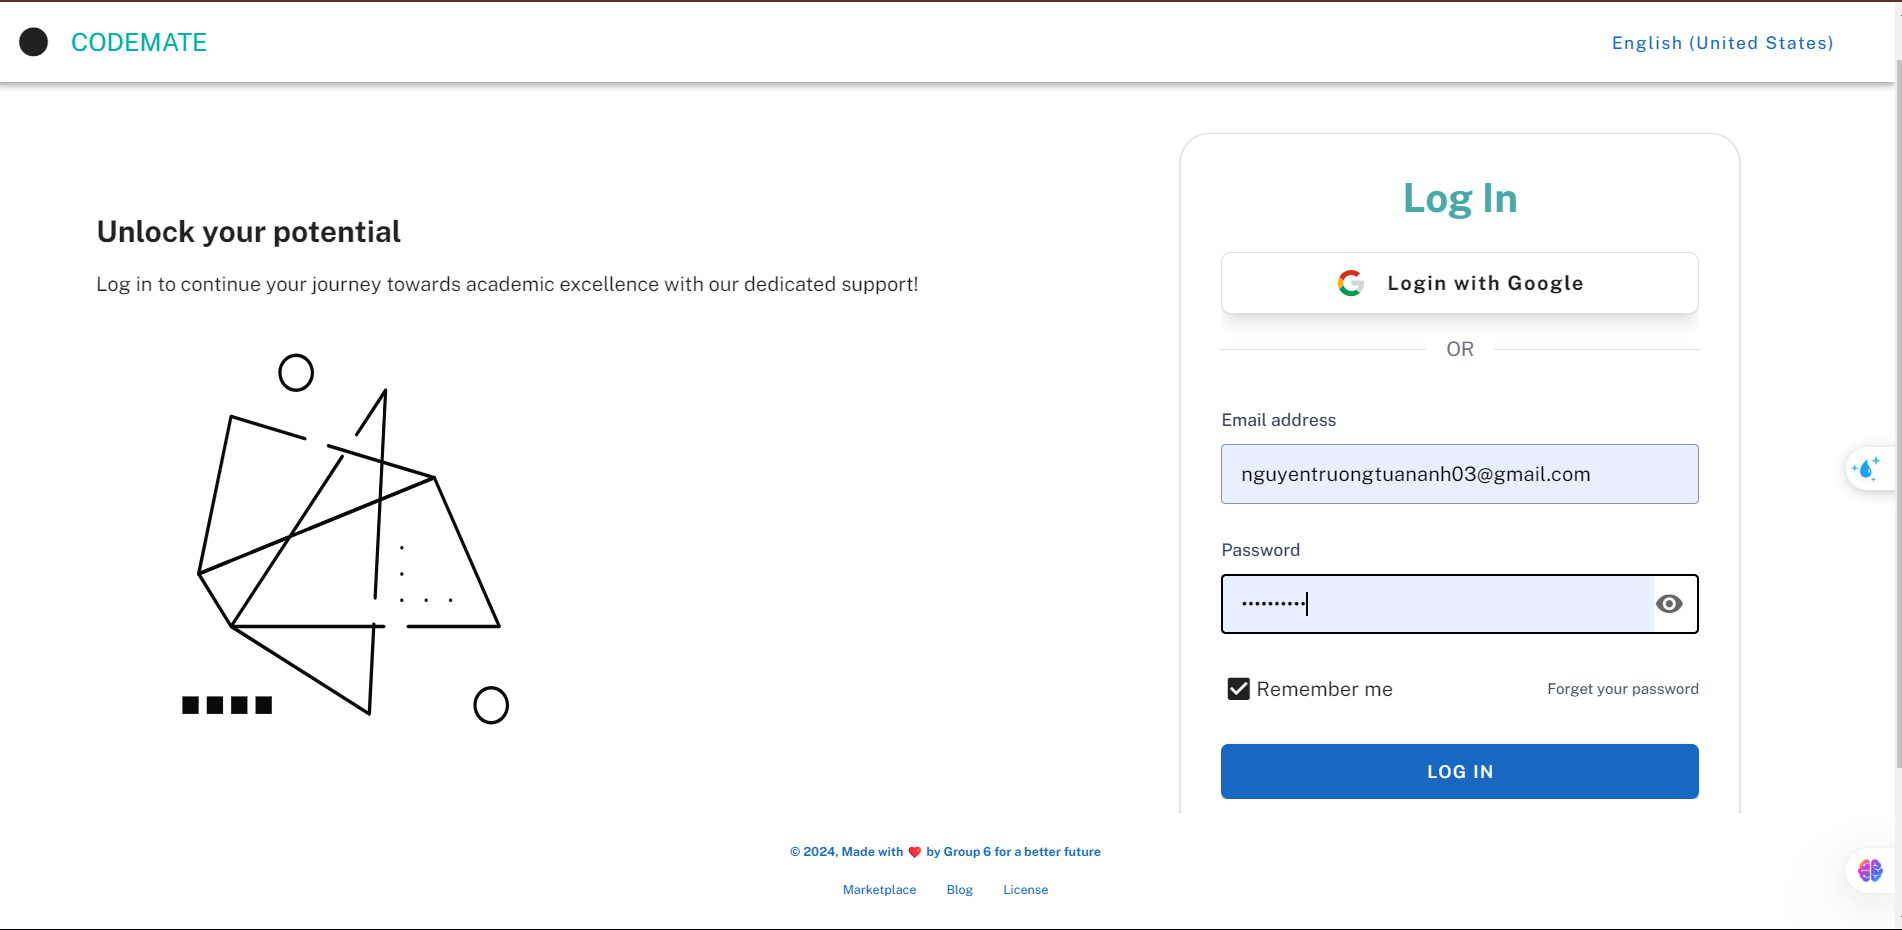
\includegraphics[width=0.8\linewidth]{images/login.png}
        \caption{Nhập tài khoản và mật khẩu}
        \label{fig:enter-label}
    \end{figure}
    \item Kiểm tra trạng thái xác thực email (is\_verified) nếu chưa tạo mã xác thực ngẫu nhiên gửi đến email người dùng.
    \begin{figure}[H]
        \centering
        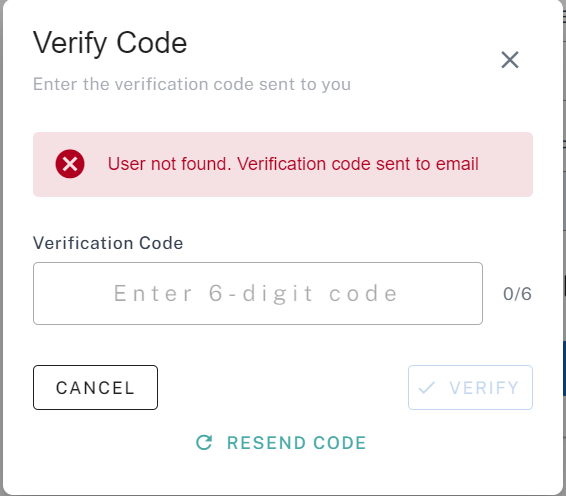
\includegraphics[width=0.6\linewidth]{images/send_code.png}
        \caption{Nhập mã code}
        \label{fig:enter-label}
    \end{figure}
    
    \item Phân quyền người dùng
\end{itemize}

% \section{Student}
\subsection{Progress Tracking}
Hệ thống theo dõi tiến độ học tập được thiết kế để giúp sinh viên nắm rõ quá trình học tập của họ trong khóa học.
\begin{itemize}
    \item Thông tin khóa học cơ bản
    \begin{itemize}
        \item Chi tiết khóa học.
        \item Tiến độ hoàn thành.
        \item Mục tiêu sinh viên trong khóa học.
        \item Learning Outcomes
    \end{itemize}
    \begin{figure}[H]
        \centering
        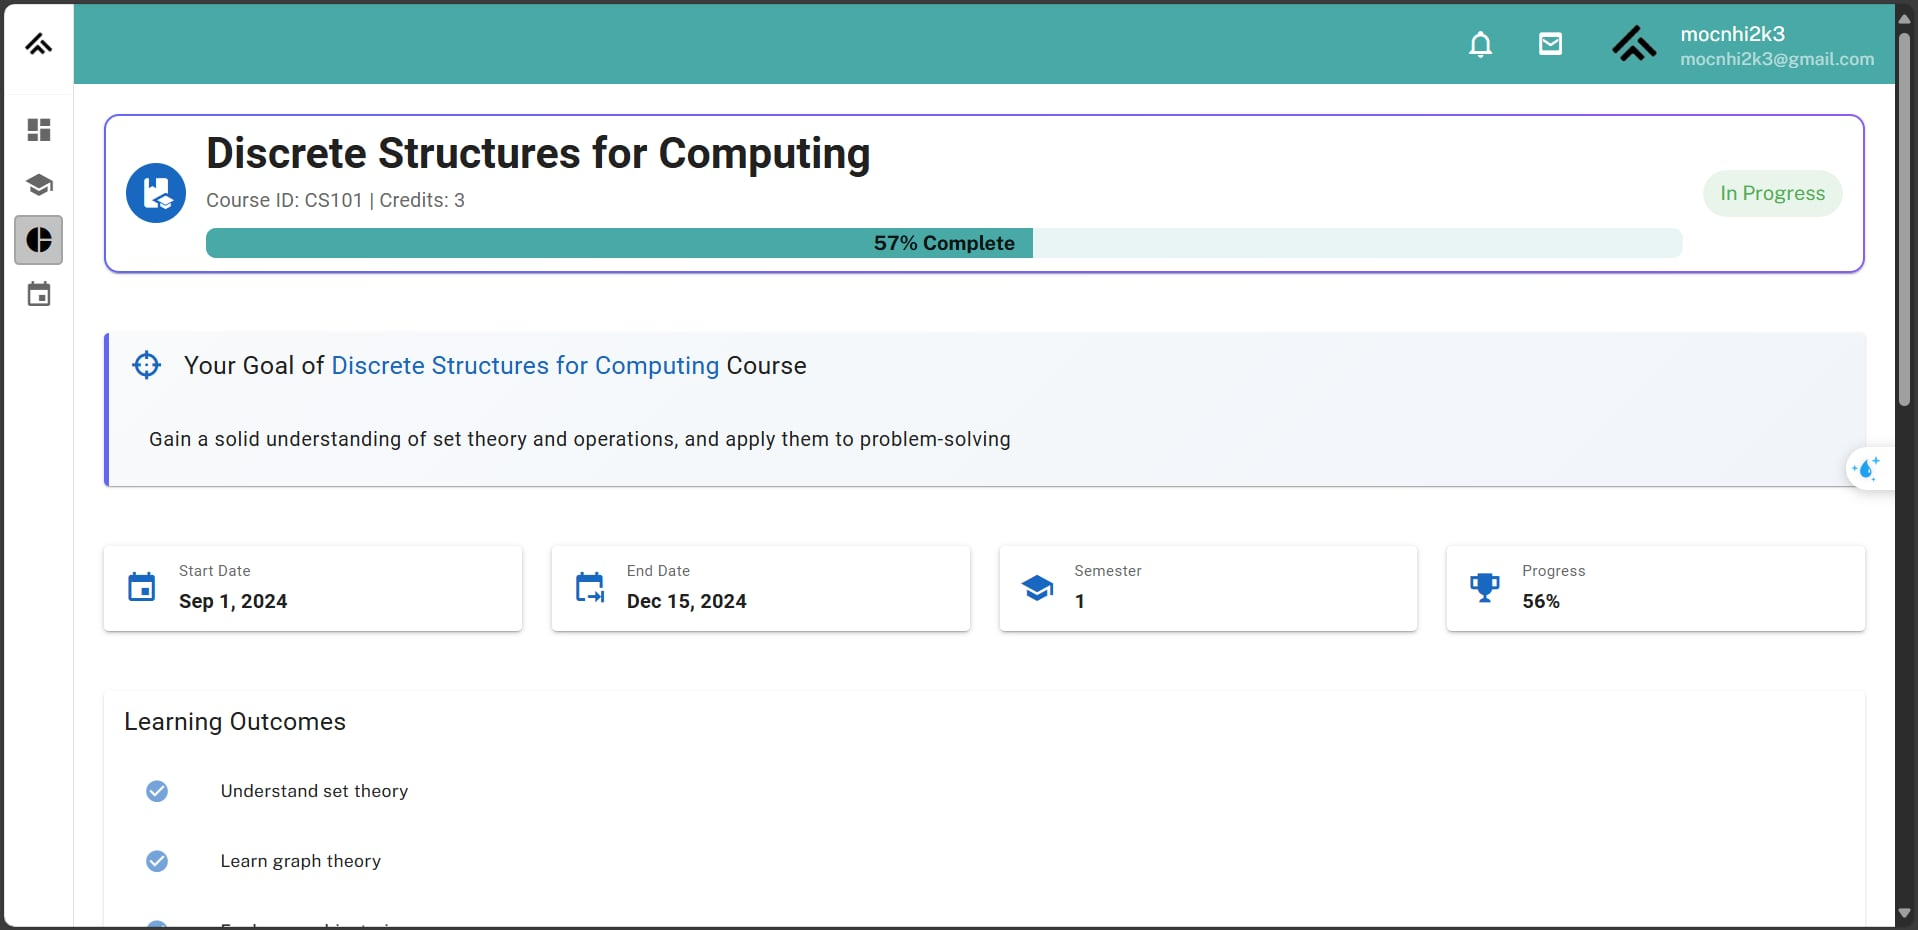
\includegraphics[width=0.8\linewidth]{images/progress_info_course.png}
        \caption{Thông tin khóa học}
        \label{fig:enter-label}
    \end{figure}
    \item Performance Metrics:
    \begin{itemize}
        \item Tỷ lệ hoàn thành bài tập
        \item Điểm số trung bình
        \item Thời gian học tập
        \item Mức độ tương tác với nội dung khóa học
    \end{itemize}
    \begin{figure}[H]
        \centering
        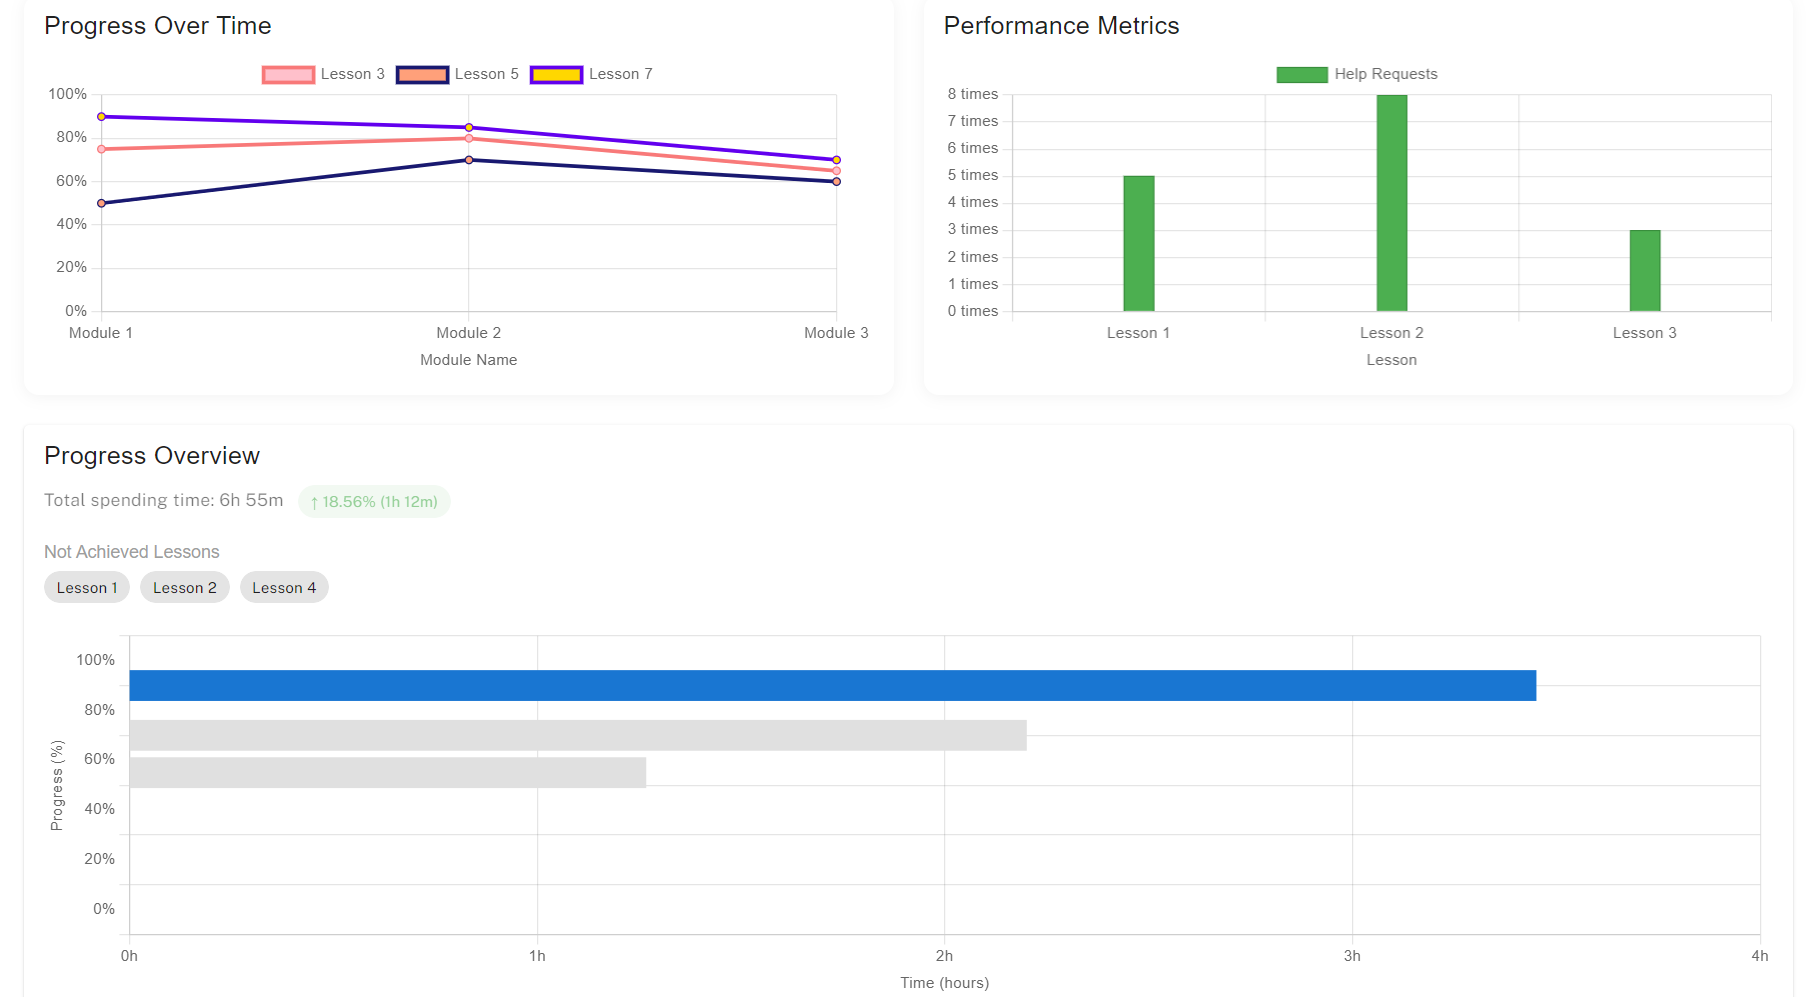
\includegraphics[width=0.8\linewidth]{images/progress_statistic.png}
        \caption{Thống kê kết quả học tập}
        \label{fig:enter-label}
    \end{figure}
\end{itemize}

% \section{Professor}
\subsection{Dashboard}
Trang Dashboard giáng viên cung cấp một giao diện trực quan giúp điều hướng đến những trang khác một cách dễ dàng gồm các thành phần chính như sau:
\begin{itemize}
    \item Thống kê giảng viên:
    \begin{itemize}
        \item Hiển thị tổng số khóa học mà giảng viên quản lý: chuyển đến trang danh sách khóa học
        \item Tổng số sinh viên đang theo học trong các khóa học: chuyển đến trang tiến độ sinh viên trong khóa học
        \item Hiển thị tổng số bài giảng mà giảng viên đã thiết lập.
        \item Hiển thị tổng số bài tập đã được giao cho sinh viên: chuyển đến trang tạo bài tập.
    \end{itemize}
    \begin{figure}[H]
        \centering
        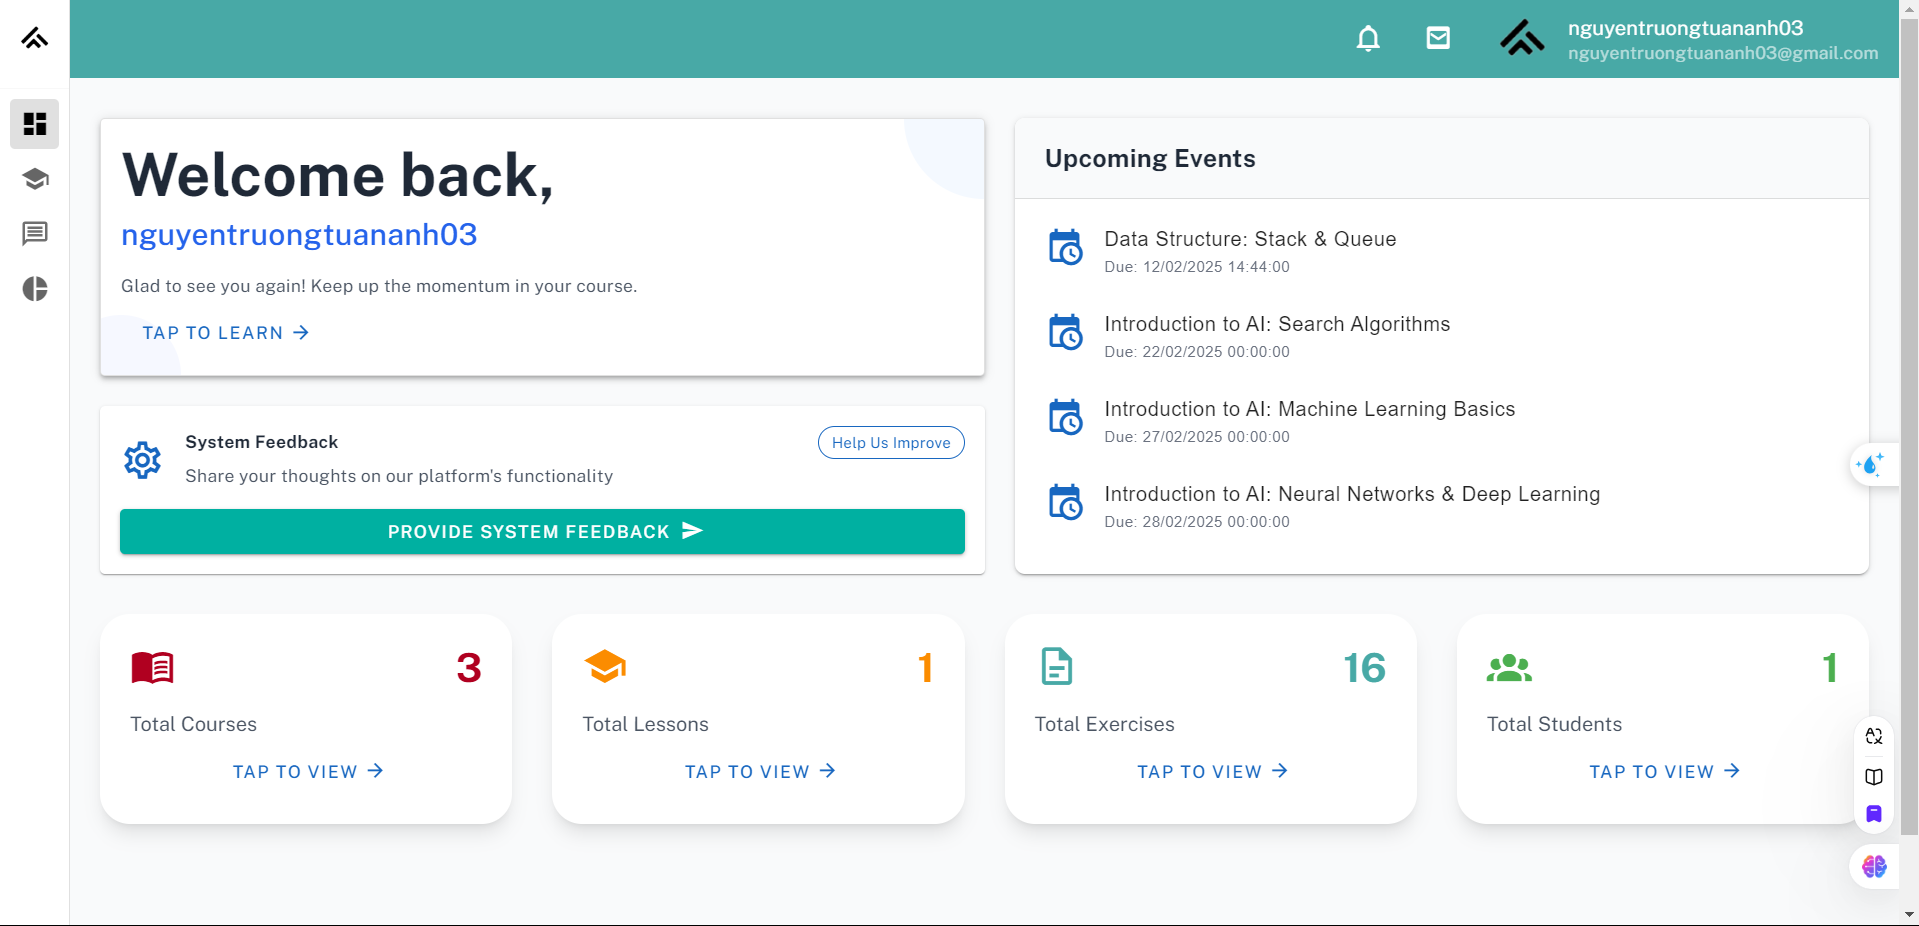
\includegraphics[width=0.8\linewidth]{images/dashboard_professor.png}
        \caption{Dashboard Professor}
        \label{fig:enter-label}
    \end{figure}
    \item Upcoming Events: hiển thị danh sách các sự kiện quan trọng sắp diễn ra mà giảng viên cần quan tâm (Hạn nộp bài tập, kỳ thi, sự kiện liên quan đến học viên)
    \item Gửi Feedback cho hệ thống: Giảng viên có thể gửi feedback về hệ thống qua một modal.
    \begin{figure}[H]
        \centering
        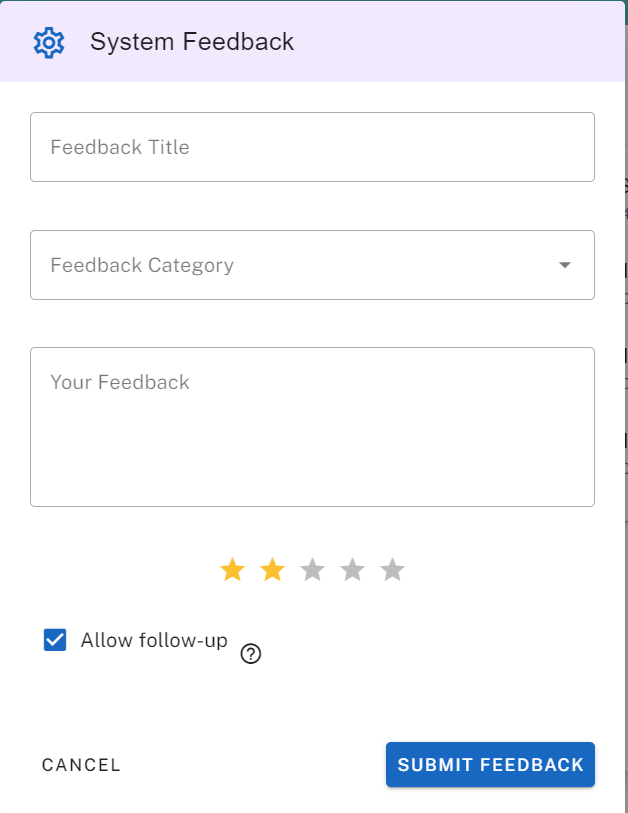
\includegraphics[width=0.3\linewidth]{images/modal_feedback.png}
        \caption{Modal Feedback}
        \label{fig:enter-label}
    \end{figure}
\end{itemize}
\subsection{My Course}
Trang My Course cung cấp danh sách các khóa học mà giảng viên phụ trách. Mỗi khóa học gồm các thông tin chi tiết như: tên khóa học, mã khóa học, sinh viên, learning outcomes, trạng thái khóa học, thời gian khóa học.
\begin{figure}[H]
        \centering
        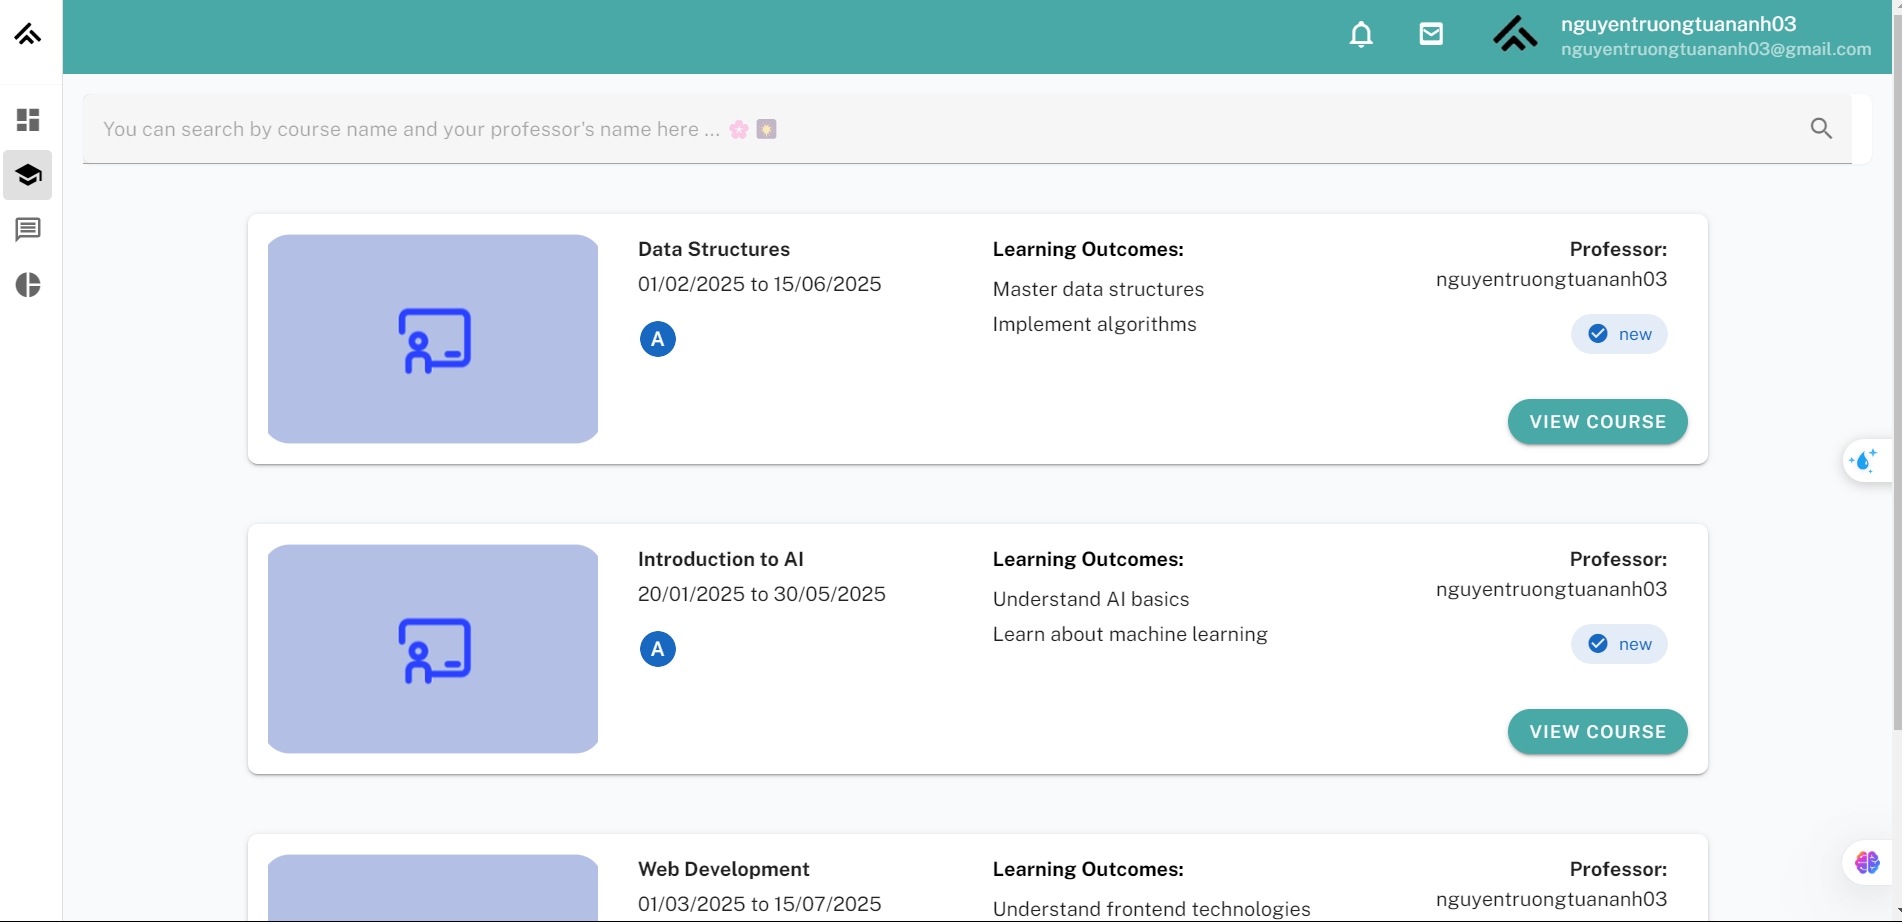
\includegraphics[width=0.8\linewidth]{images/course_professor.png}
        \caption{Professor: My Course}
        \label{fig:enter-label}
    \end{figure}
\subsection{Feedback Management}
Tính năng quản lý phản hồi giúp giảng viên theo dõi và phân tích ý kiến của sinh viên về khóa học.
\begin{itemize}
    \item Giảng viên có thể chọn một khóa học cụ thể từ danh sách các khóa học mà họ đang giảng dạy.
    \item Hệ thống sẽ hiển thị ra danh sách feedback gồm các thông tin: người gửi, tiêu đề phản hồi, mô tả, phân loại, rating.
    \begin{figure}[H]
        \centering
        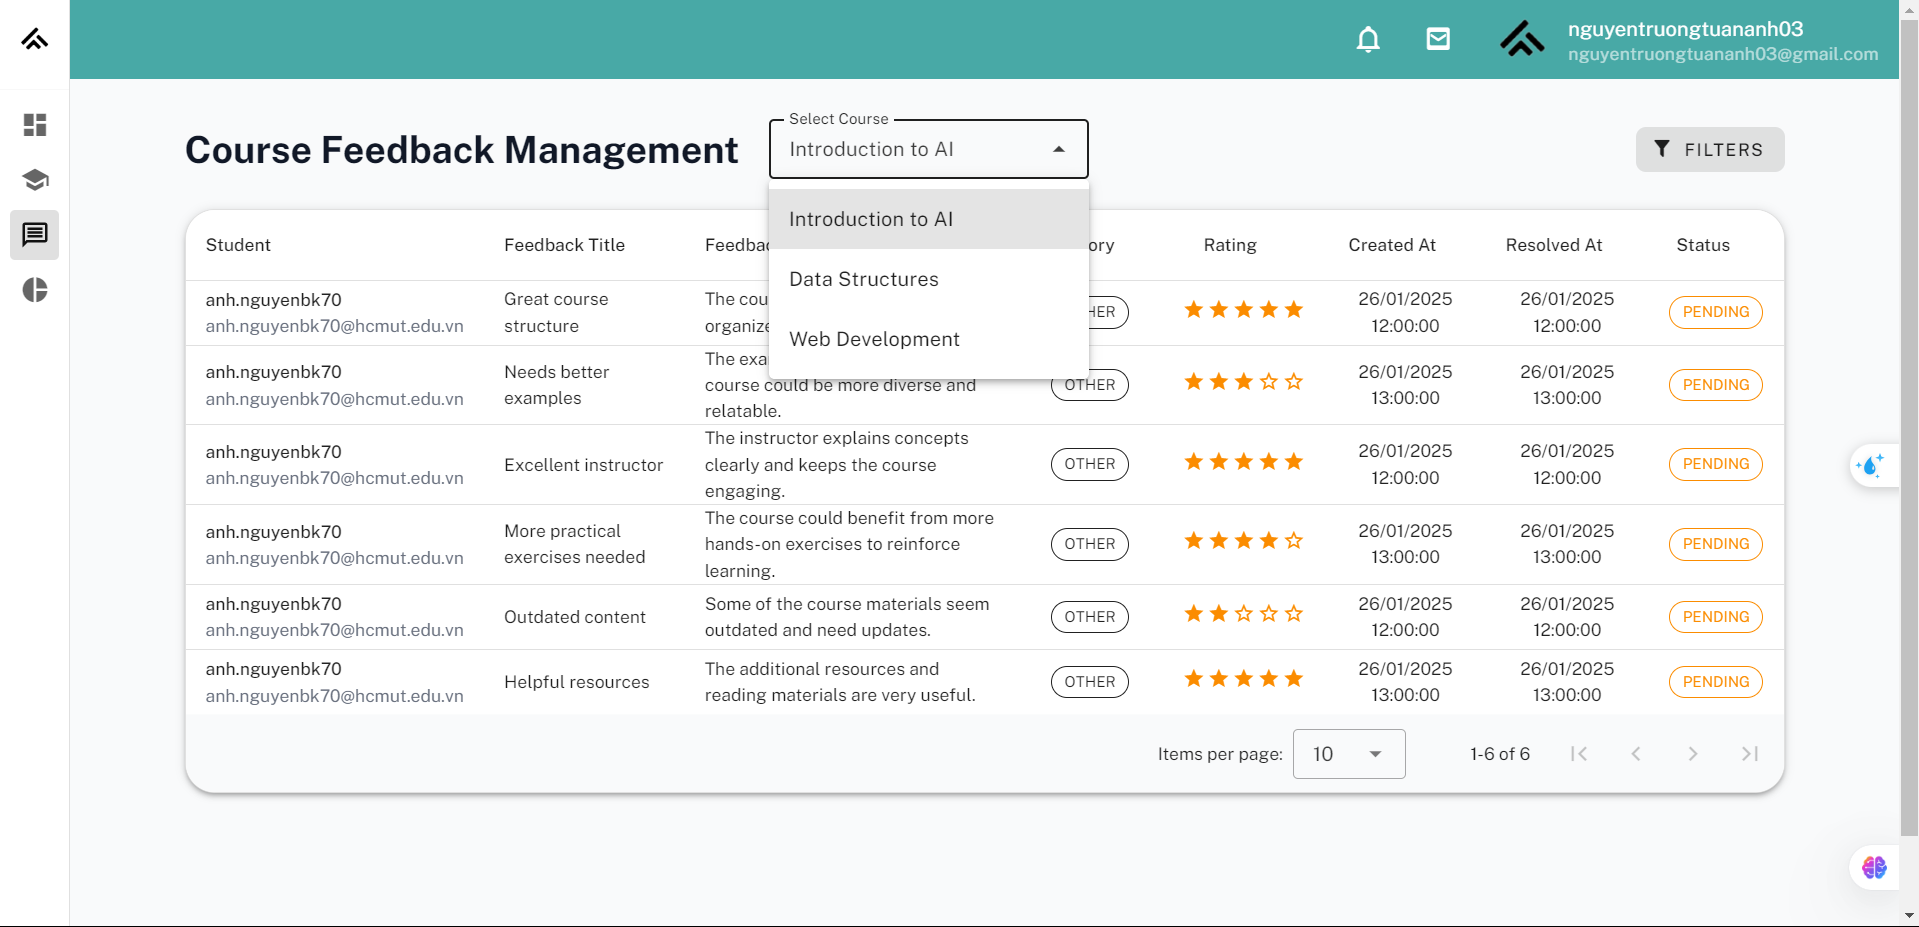
\includegraphics[width=0.8\linewidth]{images/feedback_professor.png}
        \caption{Professor: Feedback Management}
        \label{fig:enter-label}
    \end{figure}
\end{itemize}
\subsection{Progress Student}
Trang tiến độ này theo dõi tiến độ sinh viên giúp giảng viên đánh giá hiệu suất học tập của từng sinh viên trong khóa học
\begin{itemize}
    \item Tổng quan lớp học: điểm cao nhất, thấp nhất, trung bình điểm
    \item Tiến độ cá nhân: 
    \begin{itemize}
        \item Learning path cá nhân của sinh viên trong khóa học.
        \item Điểm số của từng bài kiểm tra và bài tập.
    \end{itemize}
    \item Chi tiết bài tập: Điểm của sinh viên trong bài tập, lời giải, lịch sử nộp bài và số lần thử lại.
\end{itemize}
 \begin{figure}[H]
        \centering
        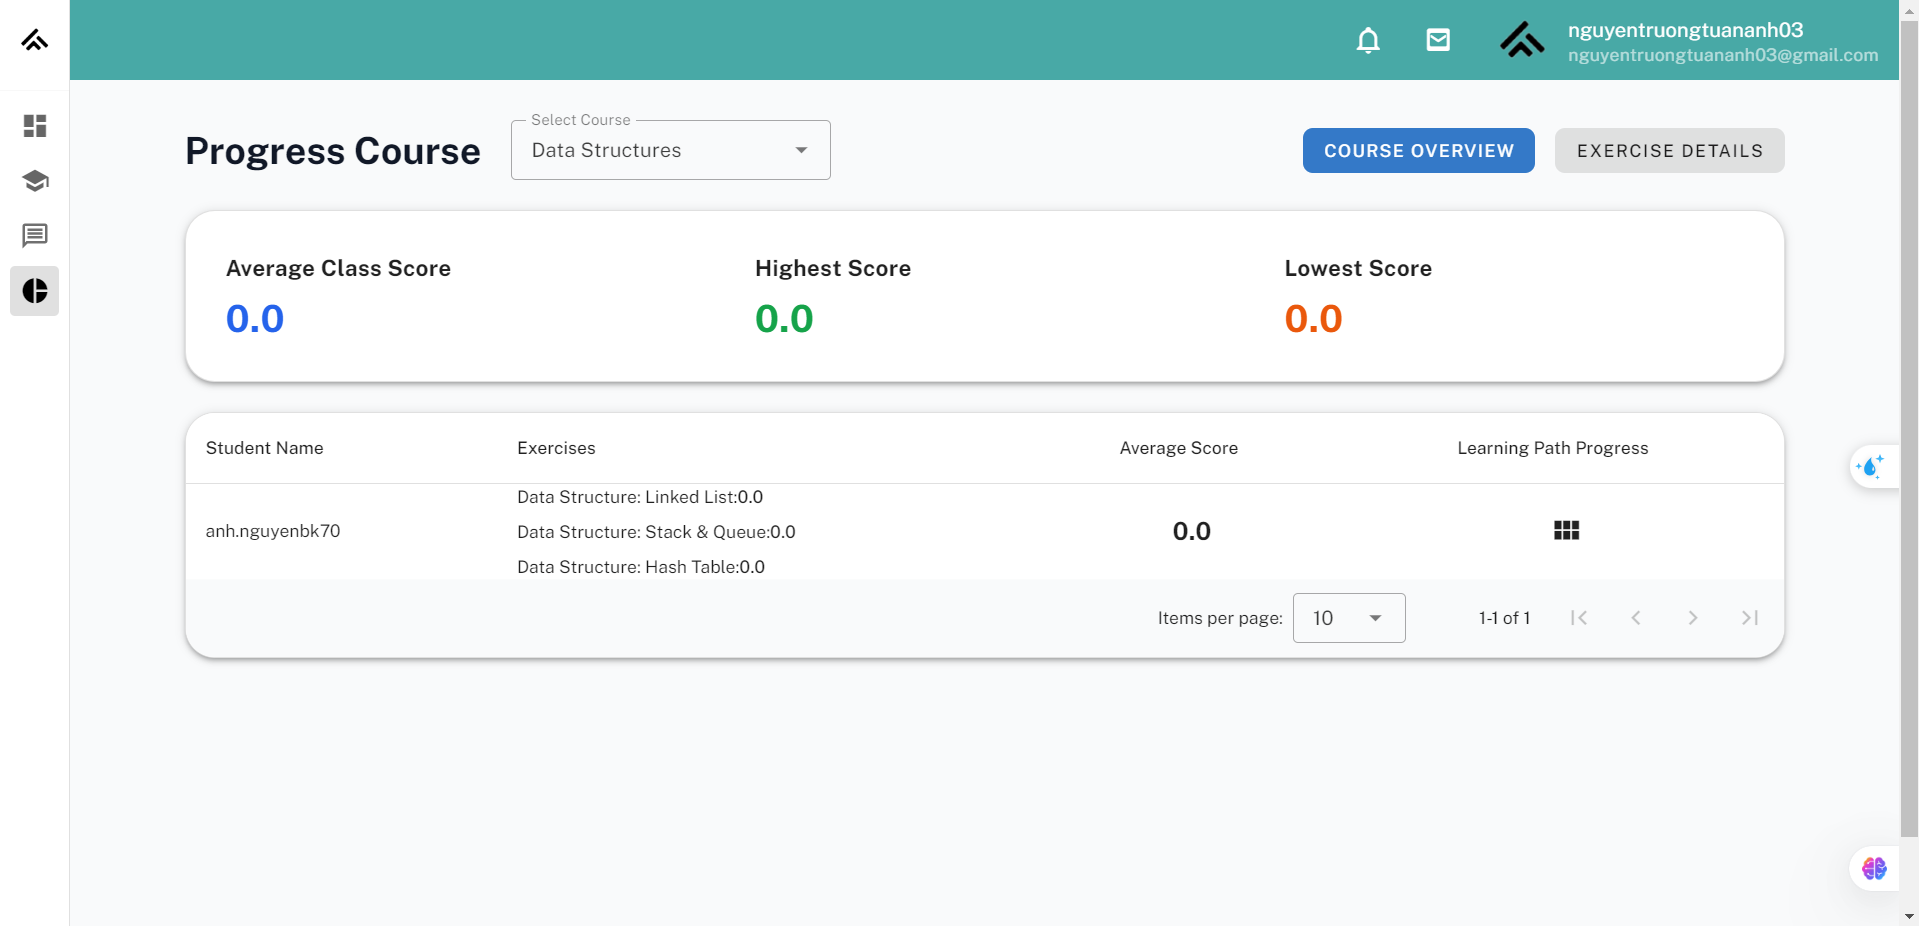
\includegraphics[width=0.8\linewidth]{images/progress_professor.png}
        \caption{Professor: Progress Student}
        \label{fig:enter-label}
    \end{figure}
% \section{Admin}
\subsection{Dashboard}
Trang dashboard của Admin đượcthiết kế để theo dõi và quản lý hiệu suất hệ thống, phân tích dữ liệu người dùng trong hệ thống học trực tuyến.
\begin{itemize}
    \item Hiệu suất hệ thống: FCP, LCP INP
    \item Số liệu tổng quan của hệ thống
    \begin{figure}[H]
        \centering
        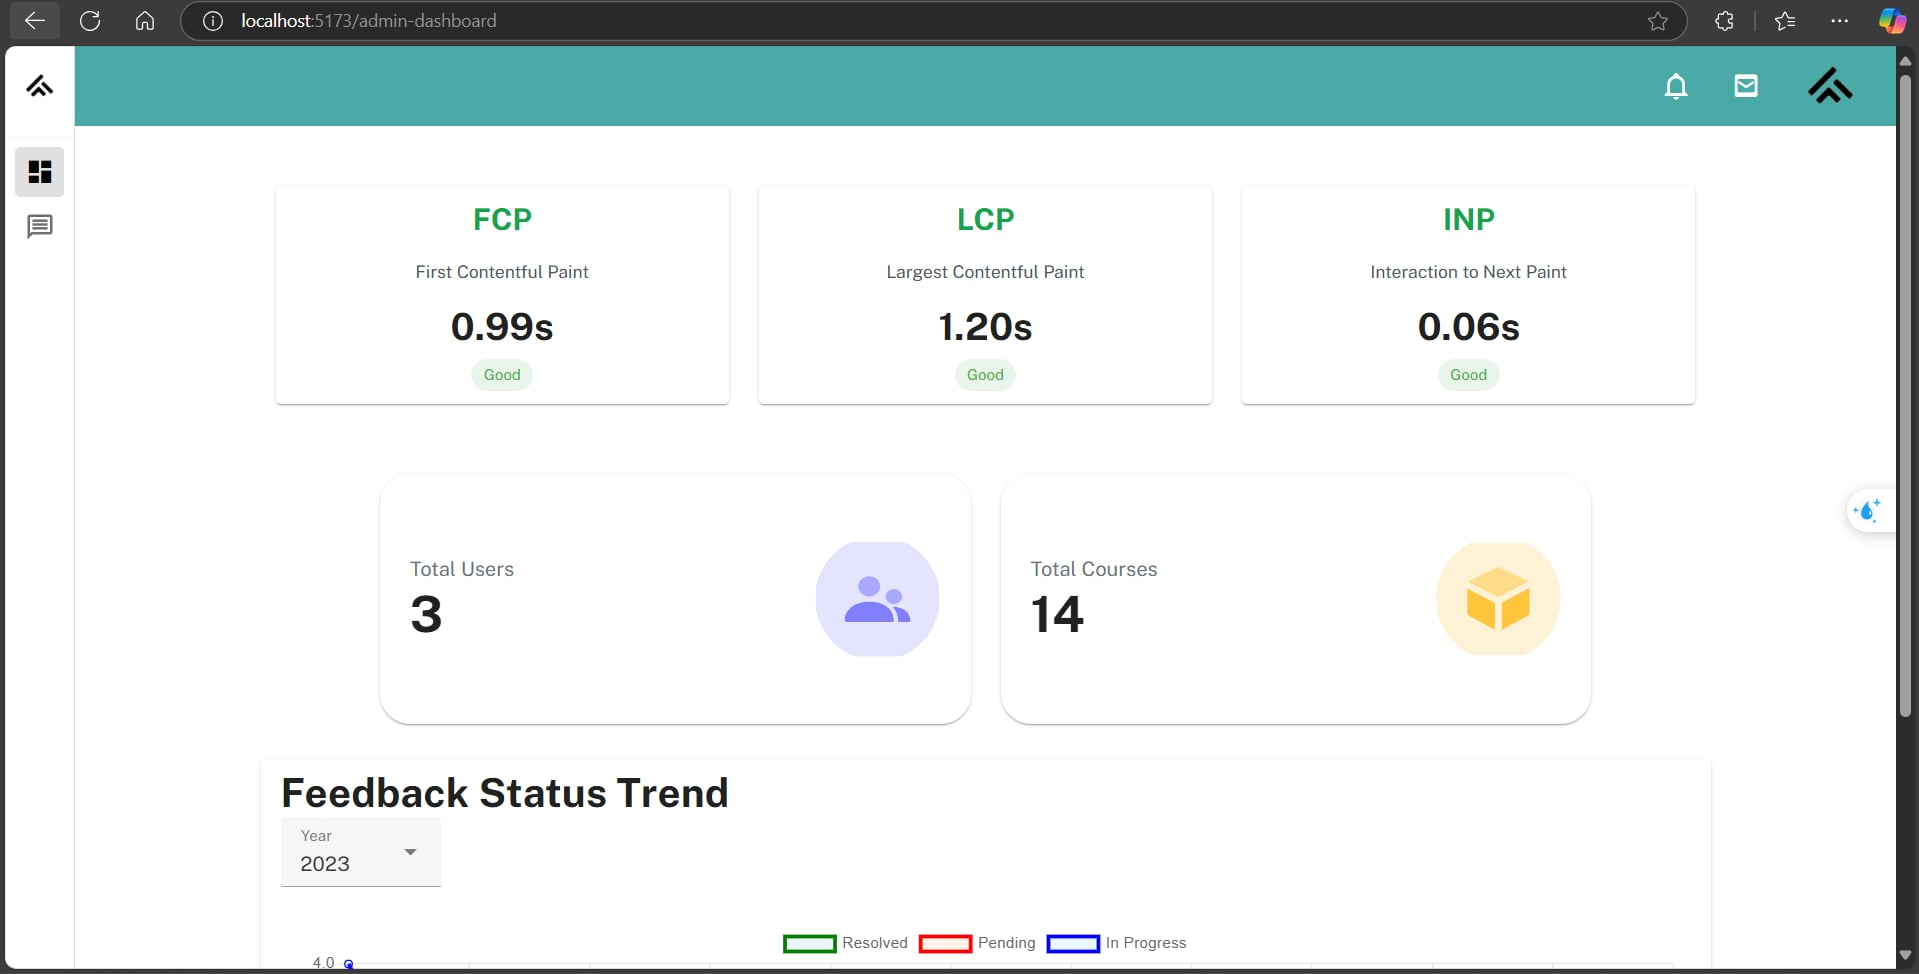
\includegraphics[width=0.8\linewidth]{images/dashboard_stat.png}
        \caption{Dashboard Admin}
        \label{fig:enter-label}
    \end{figure}
    \item Biểu đồ thống kê feedback: đã giải quyết, đang xử lí, đang chờ
    \begin{figure}[H]
        \centering
        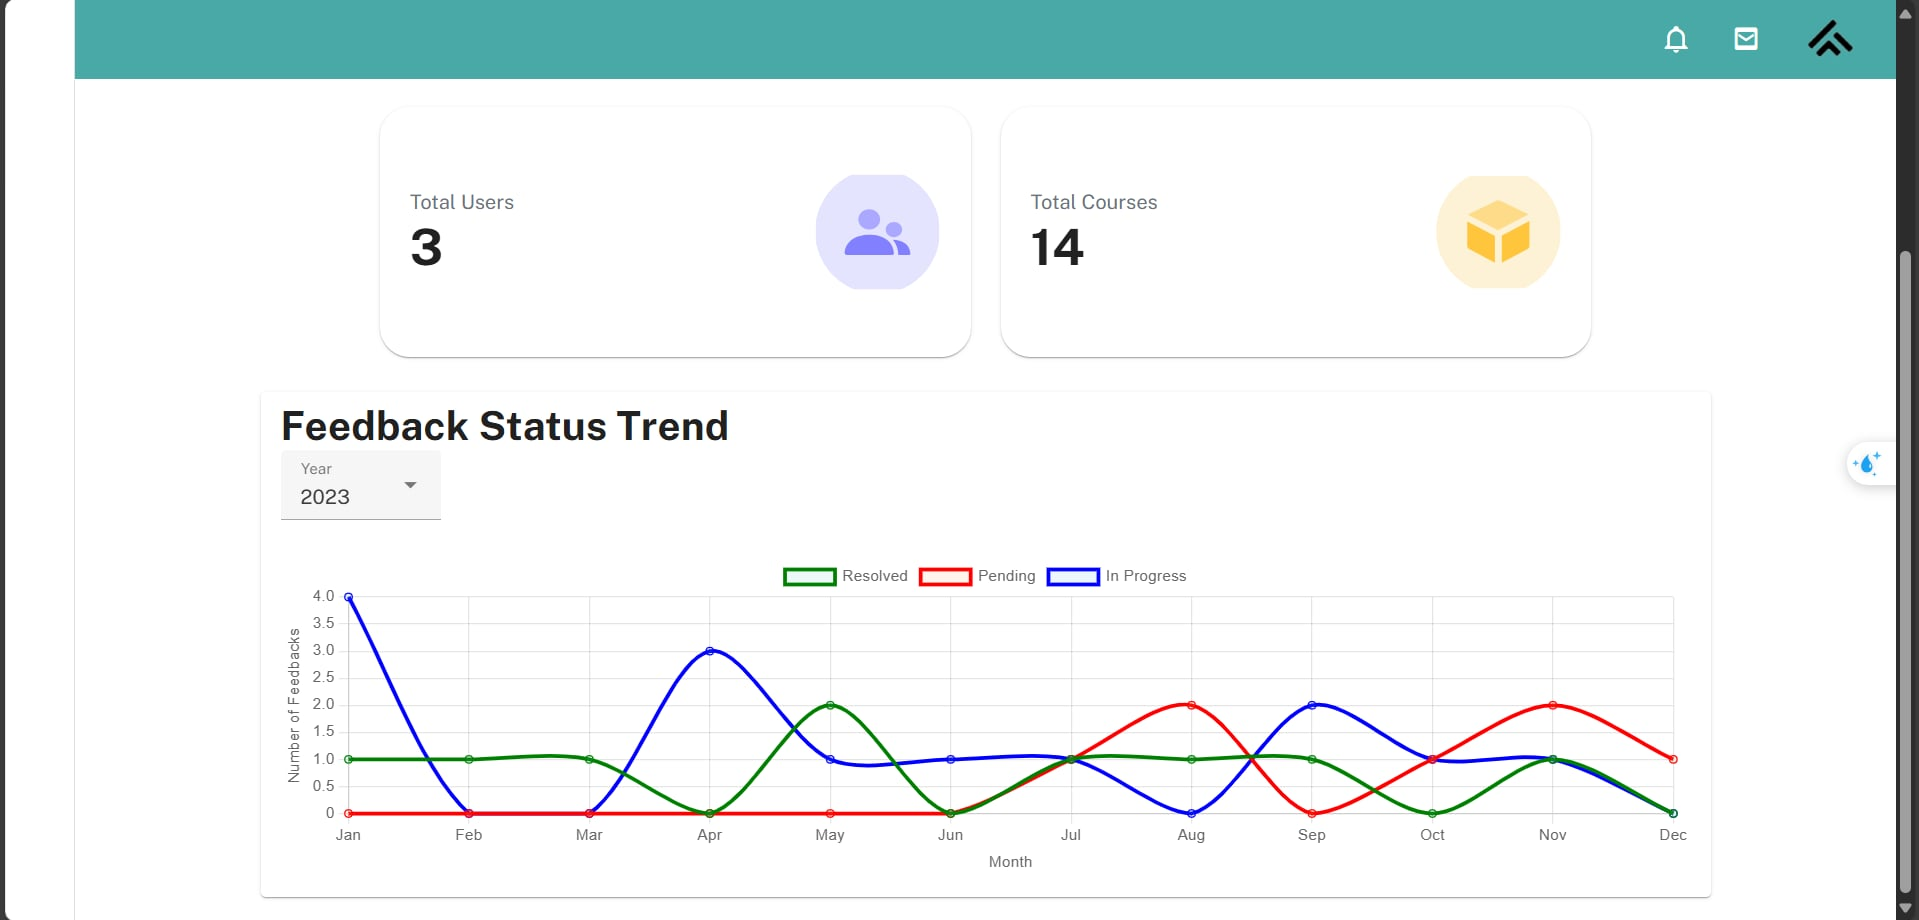
\includegraphics[width=0.8\linewidth]{images/dashboard_feedback.png}
        \caption{Biểu đồ thống kê feedback}
        \label{fig:enter-label}
    \end{figure}
\end{itemize}
\subsection{Feedback Management}
Admin có thể theo dõi và xử lý các phản hồi (feedback) từ người dùng thông qua một bảng danh sách hiển thị chi tiết từng feedback. Mỗi phản hồi bao gồm các thông tin chính như:
\begin{itemize}
    \item Người gửi (User): Tên hoặc ID của người dùng đã gửi phản hồi.
    \item Tiêu đề phản hồi, mô tả
    \item Phân loại:
    \begin{itemize}
        \item Performance
        \item Bug Report
        \item Feature Request
        \item UI/UX
        \item Others
    \end{itemize}
    \item Rating: 1-5 sao
    \item Trạng thái feedback
\end{itemize}

\begin{figure}[H]
        \centering
        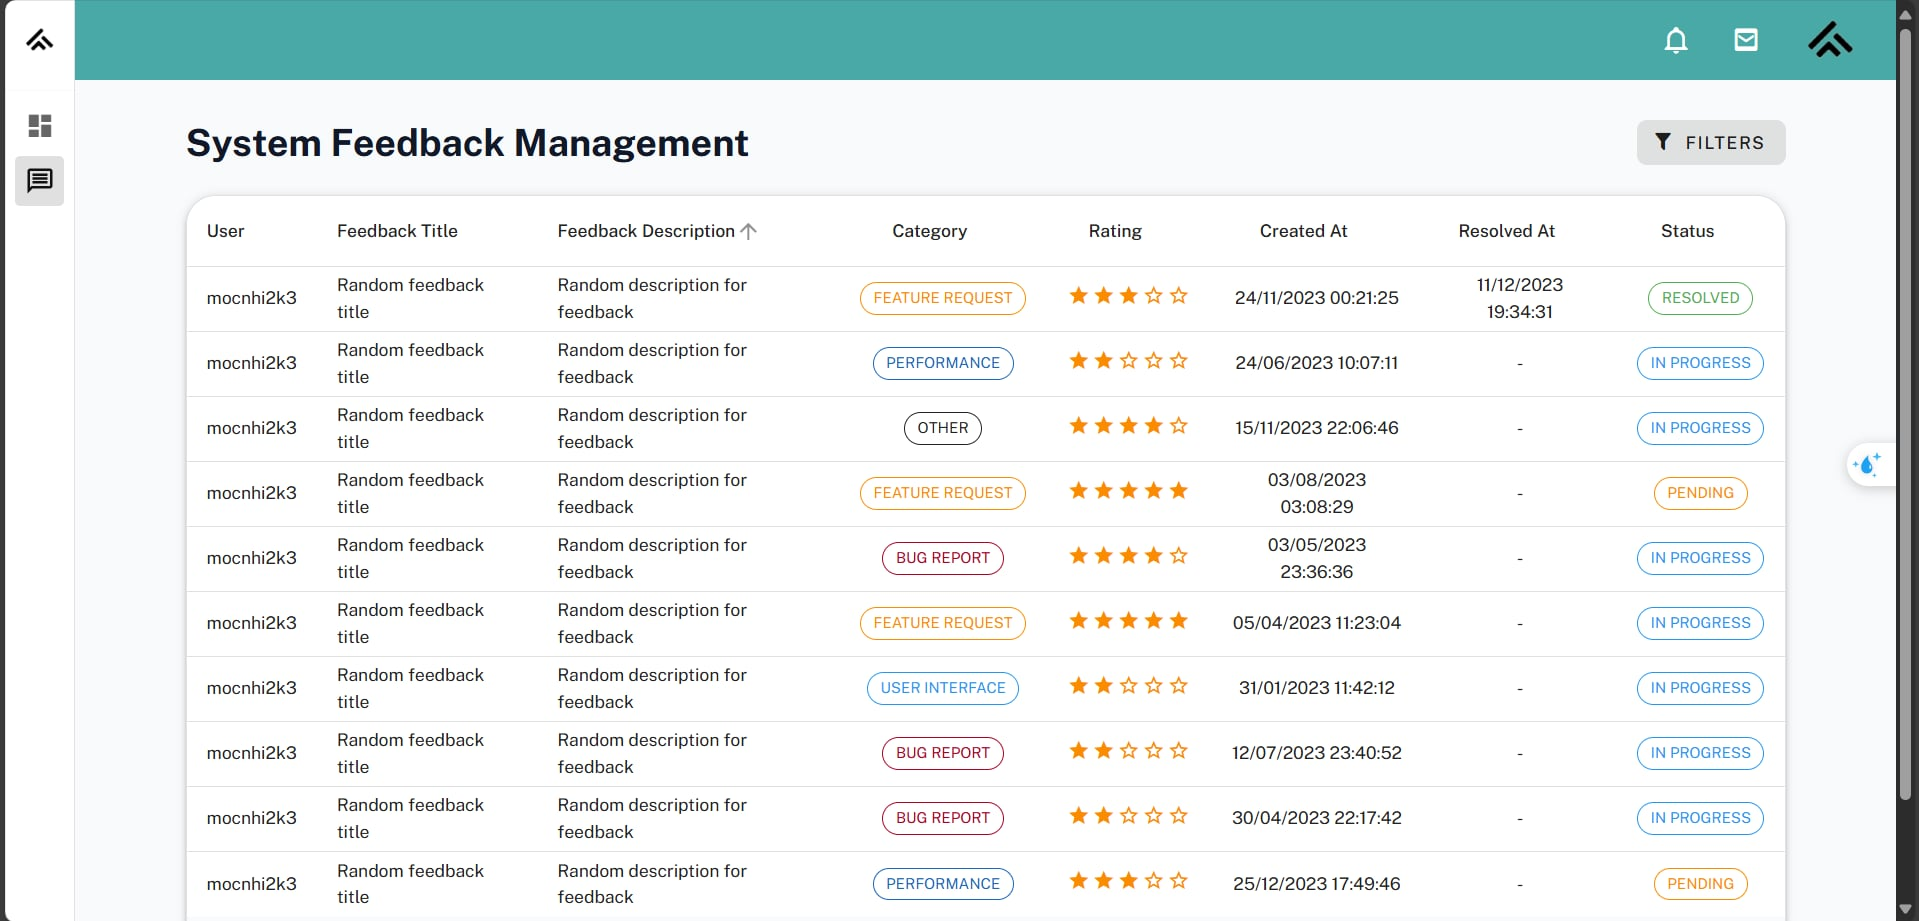
\includegraphics[width=0.8\linewidth]{images/feedback_management.png}
        \caption{Danh sách feedback của hệ thống}
        \label{fig:enter-label}
    \end{figure}
Admin có thể lọc và tìm kiếm các phản hồi dựa trên:
\begin{itemize}
    \item Khoảng thời gian nhất định.
    \item Lọc theo phân loại.
    \item Lọc theo trạng thái feedback.
\end{itemize}
\begin{figure}[H]
        \centering
        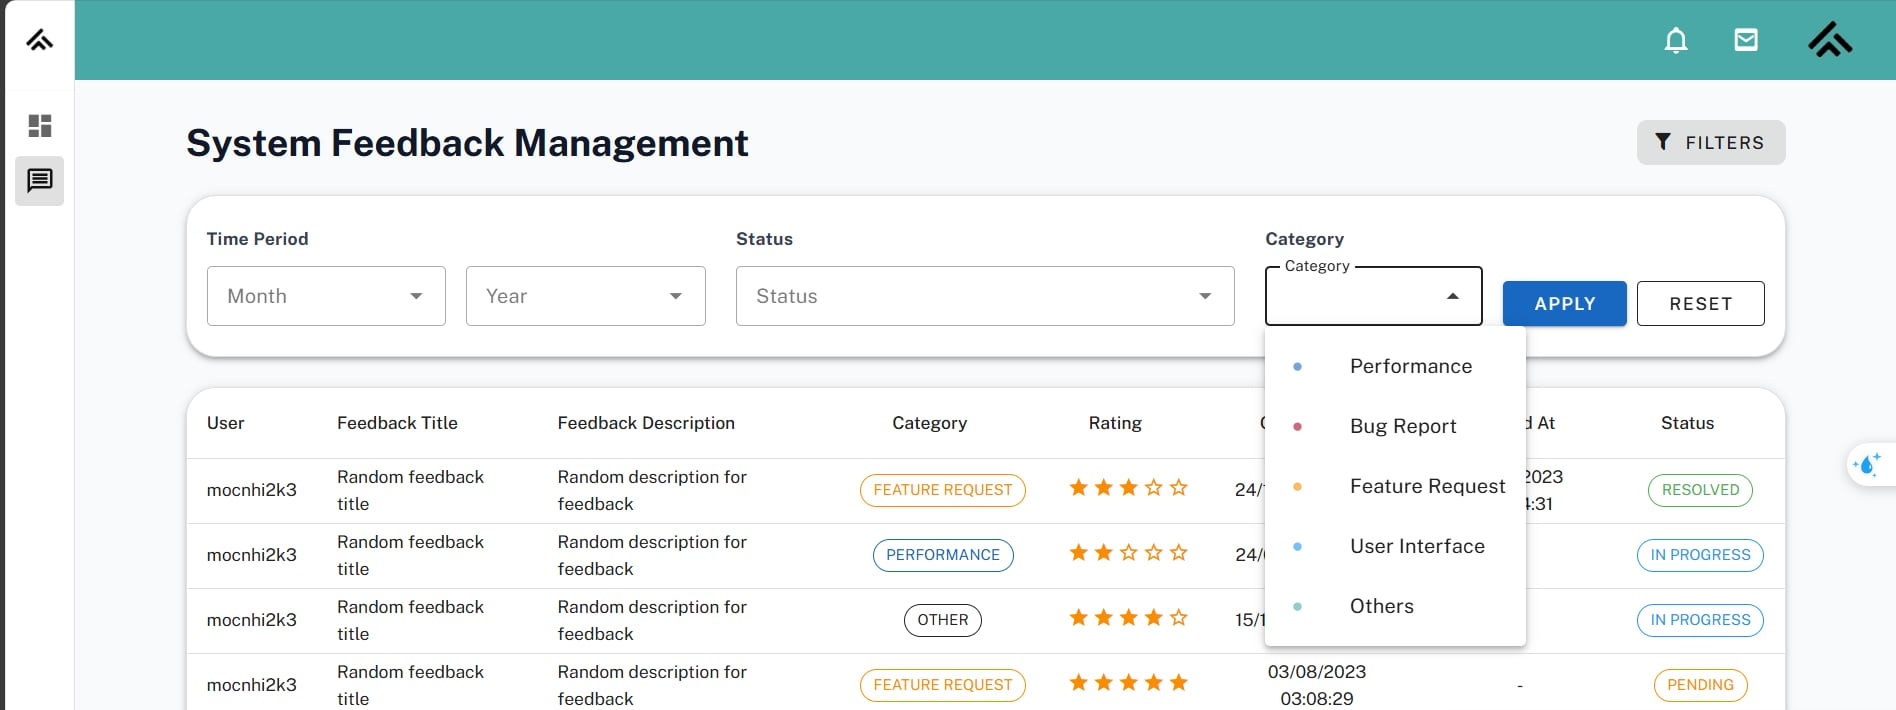
\includegraphics[width=0.8\linewidth]{images/feedback_filter.png}
        \caption{Lọc danh sách feedback}
        \label{fig:enter-label}
    \end{figure}

\end{document}